% !TEX program = xelatex
% Note: Changed from lualatex due to MiKTeX luaotfload issues
\documentclass[12pt,a4paper,oneside]{NITR}

\usepackage{listings}
\usepackage{amsfonts}
\usepackage{amssymb}
\usepackage{xcolor}
%\usepackage[linesnumbered,ruled,vlined]{algorithm2e}
\usepackage[linesnumbered,ruled,vlined,longend]{algorithm2e}
\usepackage{adjustbox}
\usepackage{tcolorbox}
\tcbuselibrary{listingsutf8}
\usepackage[hyphens]{url}

%\documentclass{article}
\usepackage{titlesec}
\usepackage{graphicx} % Required for inserting images
\usepackage[export]{adjustbox}
%\usepackage{blindtext}
%\usepackage{geometry}
%\usepackage{multirow}
%\usepackage{amsmath}
%\usepackage{indentfirst}
%\usepackage{array}
%\usepackage{url}
\usepackage{hyperref}
\usepackage{subcaption}
\usepackage{caption}
\usepackage{float}
\usepackage{listings}
\usepackage{amsfonts}
\usepackage{amssymb}
\usepackage{xcolor}
\usepackage[linesnumbered,ruled,vlined]{algorithm2e}
%\usepackage[usenames,dvipsnames]{color}
%\usepackage[colorlinks=true,breaklinks,backref=true,linkcolor={MidnightBlue},citecolor={Fuchsia},urlcolor={OliveGreen}]{hyperref}
\usepackage[none]{hyphenat}
\usepackage{amsmath,amsfonts,mathdots,amssymb,yfonts}
\usepackage{graphicx}
\usepackage{tikz}
\usetikzlibrary{trees,shapes}
\usepackage{booktabs}
%\usepackage{subfigure}
%\usepackage[ruled,linesnumbered,slide,vlined]{algorithm2e}
%\usepackage{verbatim}
%\usepackage{wrapfig}
%\usepackage{multirow}
%% % % % % % %
\onehalfspacing
\begin{document}
\sloppy
% % % % % % % % % % % % % % % % % % % % % % % % % % %
% % % % % % % % % % % % % % % % % % % % % % % % % % %
\author{Biswaranjan Dash}
\rollNumber{223CS3142}
\authorGender{male}		%%Author's gender: male or female
\department{Department of Computer Science and Engineering}
\docTitle{Studies On Probabilistic Forecasting Methods Employing Deep Learning Models}

% % % % % % % % % % % % % % % % % % % % % % % % % % % % % %
% % % % % % % % % % % % % % % % % % % % % % % % % % % % % %
% % % Use any ONE of the following three as appropriate

% \studentType{postgraduate}			
%%\studentType{postgraduate}	
%%\studentType{undergraduate}
	
% % % % % % % % % % % % % % % % % % % % % % % % % % % % % %
% % % Use any ONE of the following as appropriate

\degree{Master of Technology} 				 %%Doctor of Philosophy; 
%%\degree{Master of Arts}					 %%Master of Arts;
%%\degree{Master of Technology}				 %%Master of Technology;
%%\degree{Bachelor of Technology}			 %%Bachelor of Technology;
%%\degree{Master of Business Administration} %%Master of Business Administration;

% % % % % % % % % % % % % % % % % % % % % % % % % % % % % %
% % % % % % % % % % % % % % % % % % % % % % % % % % % % % %

% % % Mention the discipline in which the degree is awarded
\degreeIn{Computer Science and Engineering }



% % % Mention the specialization with which the degree is awarded. 
\specialization{Software Engineering}	

% % % % % % % % % % % % % % % % % % % % % % % % % % % % % %
% % % % % % % % % % % % % % % % % % % % % % % % % % % % % %

\docType{2}		%%Dissertation=1; Thesis=2; Project=3; Synopsis=4; Registration Report=5

% % % % % % % % % % % % % % % % % % % % % % % % % % % % % %
% % % % % % % % % % % % % % % % % % % % % % % % % % % % % %

\numOfSupervisors{1}

\principalSupervisor{Sibarama Panigrahi}	%%Name only

\hod{Dr. Bibhudatta Sahoo}				    %%Name only

\principalSupervisorDesignation{Professor}
\coSupervisorDesignation{Associate Professor}

% % % % % % % % % % % % % % % % % % % % % % % % % % % % % %
% % % % % % % % % % % % % % % % % % % % % % % % % % % % % %

\setDate{16}
\setMonth{May}
\setYear{2025}

% % % % % % % % % % % % % % % % % % % % % % % % % % % % % %
% % % % % % % % % % % % % % % % % % % % % % % % % % % % % %

\Font{1}	%% Times New Roman=1; Arial=2;
\setFont

% % % % % % % % % % % % % % % % % % % % % % % % % % % % % %
% % % % % % % % % % % % % % % % % % % % % % % % % % % % % %
% % % These may be used to fine tune the cover and title pages

\titlePageLineSpacing{2}
\titleWidth{.75}
\titleCoordinateX{0.16}
\titleCoordinateY{0.12}

% % % % % % % % % % % % % % % % % % % % % % % % % % %
% % % % % % % % % % % % % % % % % % % % % % % % % % %
% % % % % % % % % % % % % % % % % % % % % % % % % % %
	% %Fill details in "FrontPages.tex"
% % % % % % % % % % % % % % % % % % % % % % % % % % %
% % % % % % % % % % % % % % % % % % % % % % % % % % %
%%\coverPageSynReg		% %Needed for Synopsis Cover Page or 
						% %Registration Report Cover Page.
						% %To be used along with "\docType()".
						% %Use "\section{Introduction}\label{Guidelines}
Submission of synopsis or extended abstract is one of the mandatory requirements before submitting a doctoral or master thesis. It is not just a longer version of an abstract. It is as good as a research paper that conveys the essence of the thesis without overlooking the importance of introduction and conclusion. A synopsis should include the following~\textemdash~
\begin{itemize}
	\item Introduction
	\item Aim
	\item Method
	\item Results
	\item Conclusion
	\item Limitations
	\item References
	\item Dissemination
\end{itemize}

\noindent A synopsis is a self-contained, capsule description of the thesis that must make sense all by itself. Typical length of a synopsis should be between 5 and 10. Pages must of A4 dimension with 25mm margin on all four sides. The entire dissertation must be written using only a single font including all the texts inside graphs, figures, block diagrams, etc. While writing captions of tables and figures, the font size should be decreased by one point. Similarly, the font size of bibliography and index should also be lessened by a point. Students are advised to use the following in the body text~\textemdash
\begin{itemize}
\item[] serif fonts like Times New Roman (TNR) of size 12pt \\
or \\
\textsf{sans-serif fonts like Arial of size 11pt}. 
\end{itemize}
Needless to say that the use of font should be uniform throughout. Headings, Titles \textit{etc.} should use fonts as given below in Table~\ref{tab-fonts}.
{
\linespread{1}
\begin{table}[h]
\centering
\caption{Font sizes to be used in the dissertation}
\begin{tabular}{l C{25mm} C{25mm} c} 
\toprule
{Item} & Arial & {TNR} & {Justification}\\
\midrule\midrule
Main Text & 11 normal & 12 normal & Justified \\
\midrule
Sub-sub Heading & 11 bold & 12 bold & Left \\
\midrule
Sub Heading & 13 bold & 14 bold & Left \\
\midrule
Heading$^{\#}$ & 16 bold & 17 bold & Left \\
\midrule
Chapter Title & 22 bold & 24 bold & Center \\
\midrule
Chapter Number & 16 bold & 17 bold & Left \\
\bottomrule
\multicolumn{4}{l}{$^{\#}$Add serial number with one decimal place.} 
\end{tabular}
\label{tab-fonts}
\end{table}
}
\par The class file \texttt{NITR.cls} can be used to prepare a synopsis. One needs to invoke the statement ``\texttt{\textbackslash synopsisCoverPage}'' in the main ``\texttt{.tex}'' file with ``\texttt{\textbackslash docType(4)}'' and all necessary data in the ``\texttt{FrontPages.tex}''. The text of the synopsis can be written in ``\texttt{./SynopsisText/SynopsisText.tex}''."
						% %Comment rest.
\coverPage
\titlePage
\certificateOfExamination

%\certificateOneSupervisor		%% Comment any
\certificateTwoSupervisors		%% one of these two

\dedication
\declaration
\acknowledgment
\abstract
% % % % % % % % % % % % % % % % % % % % % % % % % % %
% % % % % % % % % % % % % % % % % % % % % % % % % % %
\tableofcontents
\cleardoublepage
% % % % % % % % % % % % % % % % % % % % % % % % % % %
% % % % % % % % % % % % % % % % % % % % % % % % % % %
\addcontentsline{toc}{chapter}{List of Figures}
\listoffigures 
% \listoffigures
\cleardoublepage
% % % % % % % % % % % % % % % % %
\addcontentsline{toc}{chapter}{List of Tables}
\listoftables
\cleardoublepage
% % % % % % % % % % % % % % % % % % % % % % % % % % %
% % % % % % % % % % % % % % % % % % % % % % % % % % %
\pagenumbering{arabic}
\pagestyle{fancy}
\renewcommand{\chaptermark}[1]{\markboth{#1}{}}
\renewcommand{\sectionmark}[1]{\markright{\textbf{Chapter \thechapter}}}
% % % % % % % % % % % % % % % % % % % % % % % % % % %
% % % % % % % % % % % % % % % % % % % % % % % % % % %
%Formatting Guidelines for Writing Dissertation.
\chapter{Introduction}\label{Guidelines}
\section{Introduction}
Forecasting is the backbone of several fields including energy management, financial markets, health care delivery, growth planning in rural areas and urban systems, as well as climate science. Better predictions enable stakeholders to foresee the future more clearly, spend their resources wisely, and make better decisions informed by data that will change business results as well as the societal good. Yet most conventional forecasting techniques, which deliver a single point estimate, can fail to account for one important factor — the uncertainty.
All predictive models carry inherent uncertainty, particularly when applied to real-world data. Point forecasts attempt to be an estimate of the future, but do not give a measure for the band of likely outcomes. As a result, predictions that don't match the observed values very well — large difference between predicted and actual behavior), can potentially lead decision makers astray to sub-optimal or risky decisions. This is especially noticeable in high-stakes areas such as predicting the weather, analyzing the stock market and resource management (where even slight errors of a forecast can lead to drastic losses or gains).
\par Probabilistic forecasting is a better alternative as it gives a range of possibilities by providing an estimate in the confidence interval in which the true value is most likely to fall. These measures help decision-makers to be ready for different situations, thus reducing risks of unpredictable events. But even though probabilistic forecasting has these clear benefits, it is currently underused in many machine learning applications. Secondly, the enormous challenge where there is no agreement over which is the best approach to use — a parametric or non-parametric approach — generally makes things even worse because neither of them provides high levels of precision and reliability across datasets.
Deep learning models are a new ensemble in the work of probabilistic forecasting. Nonetheless, there is limited literature treating the determination of-or one with a lead over another on the discriminative power of these techniques across different domains. For a particular distribution (e.g., Gaussian or Weibull) and benefit from simplicity but may not be suitable to the realities of the data. However, a class of non-parametric methods such as Quantile Regression (QR) based forecasting and Bootstrap-based forecasting do not assume any underlying distribution; but they are more flexible in general, which increases their complexity in terms of computations. As a result, approaches such as the Traditional and Advanced LUBE method appear increasingly viable for use in non-parametric forecasting; however, their accuracy may still suffer relative to more established methods.

\section{Objective}
This thesis aims to design and develop precise and dependable probabilistic forecasting methods using optimized deep learning models on quantitative time series data from diverse domains.
In particular, the objectives include:
\begin{itemize}
    \item Examination and comparative evaluation of various probabilistic forecasting approaches based on Deep Learning models across multiple datasets, including stock prices, electricity consumption, and web traffic.
    \item Development and evaluation of multiple hybrid probabilistic forecasting methods that integrate traditional approaches with DL models to enhance forecasting accuracy and applicability in real-world scenarios.
\end{itemize}



\section{Organization Of Thesis}
There are six chapters in this thesis. The six interconnected chapters are intended to
thoroughly examine Probabilistic Forecasting Methods using Deep Learning Models. From identifying the problem to developing and validating a solution, each chapter builds on the one before it to form a cohesive narrative that leads the reader through the research process. The chapters are
organized as follows:

\textbf{Chapter 1} comprises the background information and research motivation necessary to comprehend this thesis. 

\textbf{Chapter 2} contains a thorough Literature Review.

\textbf{Chapter 3} contains the six different parametric and non-parametric traditional probabilistic forecasting methods and their comparisons on five different datasets using four different evaluation metrics.

\textbf{Chapter 4} introduces the LUBE-Weibull based Hybrid Method.

\textbf{Chapter 5} introduces the LUBE-QR based Hybrid Method.

\textbf{Chapter 6} contains the conclusion of the thesis and highlights future research directions.

\chapter{Literature Review}
Probabilistic forecasting has emerged as an essential tool for managing uncertainty across multiple domains—electricity price forecasting, wind power forecasting, stock price prediction, and web traffic forecasting. Classic point forecasting techniques often do not and cannot, by their very nature, fully capture the intrinsic variability at play in these fields, making probabilistic approaches more appealing to risk-sensitive decision-making. In the area of electricity price forecasting, models that deliver probability distributions of prospective prices have become increasingly popular. Two popular probabilistic forecasting methods, namely the LUBE (Lower Upper Bound Estimation) method and QR (Quantile Regression) based method, are proposed by \cite{12} and \cite{13}, which have given rise to various other methods that have incorporated these two methods. A combined probabilistic forecasting system, CPFS, synergizing quantile regression with neural networks, has established its superiority over singular model methodologies in both interval width and coverage probability and, therefore, given more reliable forecasts \cite{9}. Similarly, Gaussian Processes have been used in wind power forecasting to help in modeling the interaction that might exist between wind power generation and meteorological conditions. \cite{10} presents a multitask Gaussian process (MTGP) method successfully applied to scenarios with scarce historical data by transferring knowledge from similar source tasks to enhance the predictions of new wind farms.

In the case of prediction for stock prices, deep learning architecture-based models such as LSTM, GRU, and CNN can effectively capture the complexity and non-linearity observed within financial markets. Other models are uncertain, and there is a need to use probabilistic methods such as QR and KDE to increase the reliability of the forecast \cite{4, 9}. Deep learning architectures, particularly Long Short-Term Memory (LSTM) networks and Gated Recurrent Units (GRU), have exhibited the ability to encompass the subtle complexities inherent in the data; however, their effectiveness can be enhanced through the use of non-parametric approaches, providing better coverage intervals and better decision-making capabilities \cite{8, 3}. The application area also includes web traffic prediction, sharing patterns with similar spiky erratic changes in stock price forecasting, which also benefits from the combination of machine learning techniques. Methods such as SVM, with the incorporation of ensemble methods, have been employed to predict web traffic, thereby allowing for the allocation of resources and strategic planning of websites within precise prediction intervals \cite{5, 7}. In addition, swarm intelligence methods, including PSO and WOA, have successfully been implemented for hybrid models in forecasting; this has improved the precision of predictions in dynamic conditions \cite{9}. The key development in this case is the implementation of hybrid models integrating probabilistic forecasting with machine learning and optimization techniques, making the establishment of higher accuracy of forecasting within these fields more achievable and providing greater resilience to data uncertainty \cite{1, 6}. In conclusion, probabilistic forecasting remains fundamental in the fight against challenges attached to volatility in industries such as energy, finance, and online services, wherein uncertainty and nonlinearity are integral to the decision-making process \cite{2, 10, 9}.

Recent advancements further underscore the potential of hybrid models. For instance, \cite{14} discuss blending climate predictions with AI models to enhance hydroclimatic variable predictability, emphasizing the benefits of combining dynamical and data-driven models. Similarly, \cite{15} propose two-stage hybrid models to address heterogeneity in time series data, demonstrating improved forecasting performance by capturing both global and local patterns. In the realm of wind power forecasting, \cite{16} introduces an adaptive quantile regression approach resilient to missing values, highlighting the importance of robustness in probabilistic models. Additionally, \cite{17} present a probabilistic forecasting method for regional solar power that incorporates weather pattern diversity, showcasing the adaptability of hybrid models to various energy domains.

Despite these advancements, several research gaps remain. Most existing methods struggle to simultaneously ensure high prediction interval coverage probability (PICP) and maintain narrow prediction intervals (PINAW). For instance, QR-based methods often produce precise but under-confident forecasts, while LUBE-based methods may offer good coverage but at the cost of excessively wide intervals. There is also a lack of standardized benchmarking across different confidence levels and datasets, making it difficult to generalize findings. Furthermore, many methods are either purely parametric or purely data-driven, limiting their robustness in real-world applications where noise and variance are high.

These limitations provide a strong motivation for the development of novel hybrid methods. By combining the strengths of LUBE-based interval estimation with statistical or deep learning-based enhancements, it is possible to strike a better balance between reliability and efficiency. For instance, hybridizing LUBE with Quantile Regression (QR) introduces complementary strengths like LUBE's high coverage with QR’s narrower interval width. Similarly, integrating LUBE with Parametric models such as the Weibull distribution enables modeling of residual uncertainty and tail behavior more effectively, improving coverage in volatile scenarios. These hybrid approaches are designed to adapt across multiple model architectures (e.g., LSTM, GRU, CNN, BiLSTM) and datasets (e.g., stock prices, electricity load, web traffic), ensuring more generalizable and practically applicable forecasting systems. Thus, the present work addresses these gaps by proposing and evaluating such hybrid probabilistic forecasting frameworks that offer robustness, adaptability, and improved decision-support capacity in uncertain environments.

\begin{table}[!ht]
    \caption{Recent Literature on Probabilistic Time Series Forecasting Methods.} \vspace{0.2cm}
    \centering
    \resizebox{\textwidth}{!}{ 
    \begin{tabular}{|p{0.5cm}|p{2.8cm}|p{2cm}|p{2cm}|p{3.2cm}|p{3.2cm}|p{2.5cm}|p{2.5cm}|}
        \hline
        \textbf{Id} & \textbf{Reference} & \textbf{Model} & \textbf{Method} & \textbf{Merits} & \textbf{Drawbacks} & \textbf{Dataset} & \textbf{Accuracy Measure} \\ \hline
        \cite{12} & Abbas Khosravi et al. (2011), IEEE transactions on Neural Networks & Neural Networks & LUBE (Lower-Upper Bound Estimation) & Produces reliable prediction intervals without assuming noise distribution. Applicable to various forecasting problems. & Tuning of custom loss functions is complex. Training instability may occur. & Benchmark time series datasets & PICP, PINAW \\ \hline
        \cite{2} & Cameron Cornell et al. (2024), Int. Journal of Forecasting & Neural Networks & Probabilistic Forecasting for Electricity Prices & Adapts well to market volatility, integrates market mechanisms in forecasting. & Model sensitivity to sudden price spikes and data availability issues. & Australian National Electricity Market (NEM) & CRPS, RMSE, PICP \\ \hline
        \cite{9} & Yan Xu et al. (2024), Computers and Industrial Engineering & Quantile Regression & Quantile Combination Forecasting & Combines multiple quantile forecasts to improve robustness and accuracy. & Complexity in selecting and weighting contributing models. & Electricity price datasets & PICP, Quantile Loss \\ \hline
        \cite{1} & Sourav Kumar Purohit and S. Panigrahi (2024), Information Sciences & Hybrid (Statistical + DL) & Optimized Deep Learning & Integrates classical and deep models for improved oil price forecasting. & High computational demand; interpretability challenges. & Crude oil market datasets & RMSE, MAE, PICP \\ \hline
        \cite{3} & Hao-Hsuan Huang and Yun-Hsun Huang (2024), Energy Reports & Deep Learning & Probabilistic Forecasting with Weather Diversity & Accounts for weather diversity in regional solar forecasting. Enhances generalization. & Relies heavily on accurate meteorological inputs. & Regional solar power datasets & PICP, PINAW, RMSE \\ \hline
    \end{tabular}
    }
    \label{tab:consolidated_lit_review}
\end{table}


Table ~\ref{tab:consolidated_lit_review} summarizes recent literature on probabilistic time series forecasting methods. It highlights key studies involving different models and approaches, such as Neural Networks with LUBE, Quantile Regression, Hybrid statistical-deep learning methods and deep learning techniques tailored for specific applications like electricity price and solar power forecasting. For each reference, the table outlines the main merits and drawbacks, datasets used, and accuracy measures employed. This consolidated view provides insight into the strengths and limitations of various probabilistic forecasting methods across diverse domains, guiding future research directions.

\thispagestyle{empty}
\cleardoublepage
% % % % % % % % % % % % % % % % % % % % % % % % % % %
% % % % % % % % % % % % % % % % % % % % % % % % % % %
\input{Chap02/literature}
\chapter{Parametric and Non-parametric Probabilistic Forecasting Methods Employing Deep Learning Models} \label{Unstructured} 

\section{ Motivation}
Forecasting is crucial across many fields, from energy management and finance to medicine and climatology. Accurate predictions allow stakeholders to allocate resources in turn and make intelligent choices. Traditional forecasting techniques, however, provide single-point estimates that omit uncertainty, which can lead to suboptimal or even detrimental choices, especially in high-stakes applications such as weather forecasting and financial markets. In this chapter, we aim to conduct a study on the various existing parametric and non-parametric probabilistic forecasting methods using deep learning models across a variety of datasets to assess performance using various metrics.

Probabilistic forecasting is a better option because it provides confidence intervals that allow decision-makers to plan for a range of potential outcomes and control risks. The technique, however, is not yet a widespread practice in machine learning, partly due to the lack of a shared understanding of the optimum method. While parametric techniques (e.g., Gaussian, Weibull) are simpler to apply, they might not be able to capture data complexities fully; non-parametric techniques (e.g., Quantile Regression, Bootstrap based, etc.), conversely, are more adaptable but demand more comprehensive computational resources.

Non-parametric techniques, such as the Traditional and Advanced LUBE methods, have drawn interest as well, but accuracy remains an issue compared to traditional methods. The growing significance of machine learning to probabilistic forecasting highlights the need for more research to determine the most effective methods across different applications.

Figure \ref{fig1} presents a classification of traditional probabilistic forecasting methods and Table \ref{tab:dataset_summary} represents the datasets used in this Thesis and their length.

\begin{table}[!ht]
    \caption{Summary of Datasets Used.}
    \centering
    \begin{tabular}{|p{5cm}|c|}
        \hline
        \textbf{Dataset Name} & \textbf{Length of Dataset} \\
        \hline
        \multicolumn{2}{|c|}{\textbf{Nifty50 Dataset (2000--2021)}} \\
        \hline
        Adani Ports & 3322 \\
        Asian Paints & 5306 \\
        Axis Bank & 5306 \\
        \hline
        Web Traffic & 550 \\
        Electricity Consumption & 1858 \\
        \hline
    \end{tabular}
    \label{tab:dataset_summary}
\end{table}


\section{ Methodology}
\begin{figure*}[!t]
    \centering
    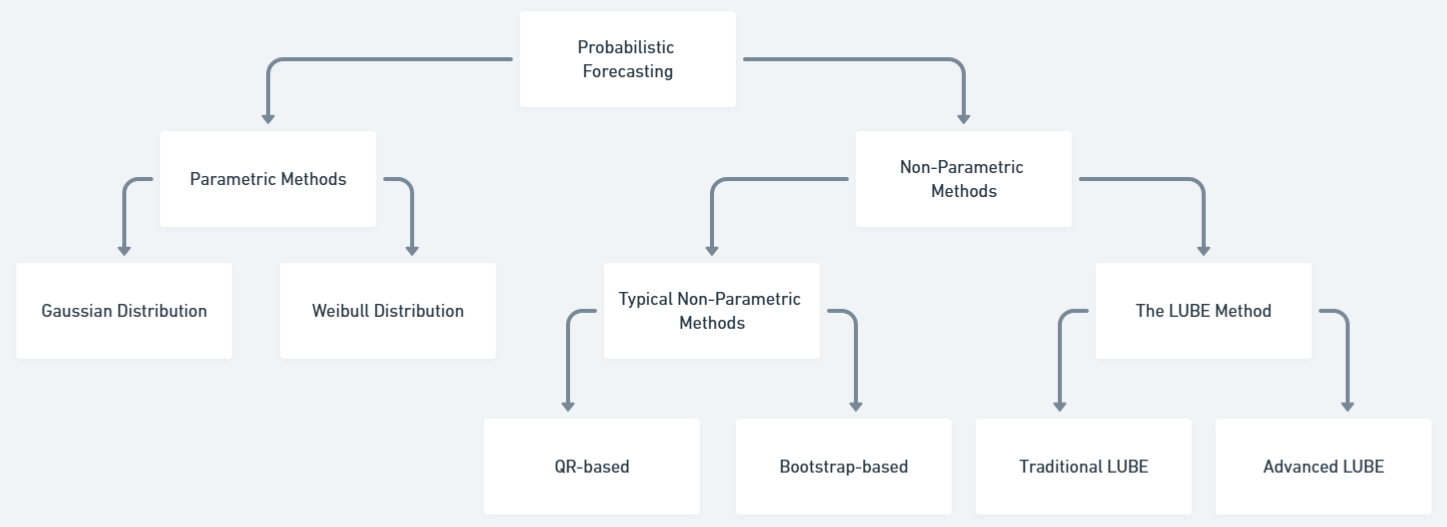
\includegraphics[width=15cm]{Chap02/Classification Of Probabilistic Methods.jpg}
    \caption{Classification of Traditional Probabilistic Methods.}
    \label{fig1}
\end{figure*}

\subsection{ Categorization Of Methods}
In this paper, six probabilistic forecasting methods are compared, broadly classified into parametric and non-parametric, each capable of producing prediction intervals (PIs) representing uncertainty in time series forecasting. Parametric methods are based on assumptions of underlying data distribution. The Gaussian (Normal) distribution-based method assumes symmetric, bell-shaped data and builds PIs from mean and standard deviation of forecast values and thus is optimal for datasets having normally distributed errors. The Weibull distribution-based method is more general and especially suited for skewed data and finds extensive use in reliability analysis and applications dealing with extreme values or variability in the data. Non-parametric methods make fewer distributional assumptions and thus find broader applicability for a wide variety of datasets. The Quantile Regression (QR)-based method estimates quantiles directly (e.g., 0.1 and 0.9 for a 90\% confidence level) to build PIs and provides robustness to non-linearity and heteroscedasticity. The Bootstrap-based method employs resampling of training data to make multiple forecasts and estimates PIs on the basis of percentiles of the resampled outputs and hence captures model and data dependent uncertainties effectively. The Traditional LUBE method builds PIs upon a custom loss function to reduce interval width and ensure adequate coverage, trading off tightness and reliability of intervals. The Advanced LUBE method builds on this by optimizing performance using novel metrics like Absolute Coverage Error (ACE) and Absolute Width Error (AWE), providing more robustness to outliers and stability at multiple confidence levels. These methods, collectively, provide a comprehensive probabilistic forecasting framework under a wide range of data conditions and uncertainty profiles.

\subsection{ Deep Learning Models}
To implement the aforementioned probabilistic forecasting techniques, four deep learning models were utilized: Long Short-Term Memory (LSTM), Gated Recurrent Unit (GRU), Convolutional Neural Network (CNN) and Bidirectional LSTM (BiLSTM). LSTM is a recurrent neural networks (RNNs) architecture specifically developed to learn long term temporal relationships in sequential data and is hence well suited for time series with intricate temporal patterns. GRU is a compact version of LSTM and hence possesses similar capabilities but lower computational complexity and is thus suitable for applications with low memory demands. CNNs, while initially developed for spatial data, have been used successfully for time series by encoding temporal sequences as structured inputs, allowing strong feature extraction through localized pattern detection. BiLSTM is an extension of LSTM with the ability to process input sequences in both directions and hence extract contextual information from past and future time steps for enhanced forecasting accuracy. These architectures were chosen based on their proven efficiency in time series forecasting tasks and their compatibility with both parametric and non-parametric probabilistic techniques.


\subsection{ Methodology}
\begin{itemize}
    \item \textbf{Dataset Preparation}
    In all the approaches described in the present study, the data preparation was performed consistently. Five different datasets were used, three stock price datasets of Nifty50 Dataset (2000-2021): Adani Ports, Asian Paints and Axis Bank and two other datasets: the Electricity Consumption dataset and the Web Traffic dataset \ref{tab:dataset_summary}. The respective target variables for prediction were 'VWAP' for the stock price datasets, 'Consumption' for the electricity dataset, and 'Views' for the web traffic dataset. The target variables were normalized first with Min-Max Scaling to provide stable convergence of the models. Next, a sliding window technique was employed to transform the time series data into a supervised learning format, thus generating several input-output pairs suitable for model training. The generated records were divided equally into training, validation, and test sets using a 70:15:15 ratio for all experimental protocols.

    \item \textbf{Evaluation Metrics}
    In this thesis, we have used the following Evaluation Metrics for fair comparison across all the methods:\\
    1. PICP (Prediction Interval Coverage Probability):\\
    Quantifies the proportion of actual values that are contained within the defined prediction intervals.
    \begin{equation}
    \begin{aligned}
    \text{PICP} = \frac{\text{Number of samples where } LB_i \leq y_i \leq UB_i}{n}
    \end{aligned}
    \label{Equation 1}
    \end{equation}
    Where:\\ 
    $y_i$: The actual observed value at time step $i$.\\
    $LB_i$: The predicted \textbf{lower bound} of the prediction interval at time step $i$.\\
    $UB_i$: The predicted \textbf{upper bound} of the prediction interval at time step $i$.\\ \\
    2. PINAW (Prediction Interval Normalized Average Width):\\
    This metric assesses the precision of the intervals.
    \begin{equation}
    \begin{aligned}
    \text{PINAW} = \frac{\frac{1}{n} \sum_{i=1}^n (UB_i - LB_i)}{\max(y) - \min(y)}
    \end{aligned}
    \label{Equation 2}
    \end{equation}
    Where:\\ 
    $n$: Total number of forecasted data points or time steps.\\
    $\max(y)$, $\min(y)$: The maximum and minimum values of the observations $y_i$ across all $n$ samples. These are used to normalize the interval width in PINAW.
    \\ \\
    3. ACE (Absolute Coverage Error):\\
    Defines the difference between actual coverage and nominally assumed confidence.
    \begin{equation}
    \begin{aligned}
    \text{ACE} = |\text{PICP} - c|
    \end{aligned}
    \label{Equation 3}
    \end{equation}
    Where $c$: The nominal confidence level of the prediction interval (e.g., 0.90 for a 90\% confidence interval).
    \\ \\
    4. AWE (Average Weighted Error):\\
    PICP and PINAW combined into an evaluation metric that is weighted.
    \begin{equation}
    \begin{aligned}
    \text{AWE} = \left| \frac{1}{n} \sum_{i=1}^n (UB_i - LB_i) - (\max(y) - \min(y)) \right|
    \end{aligned}
    \label{Equation 4}
    \end{equation}
    \\

    Eq. \eqref{Equation 1} represents the PICP evaluation metric, Eq. \eqref{Equation 2} represents the PINAW evaluation metric, Eq. \eqref{Equation 3} represents the ACE evaluation metric and finally Eq. \eqref{Equation 4} represents the AWE evaluation metric. These four metrics is used throughout this thesis to compare and evaluate perfromance of the different methods.

    \item \textbf{Output Generation}
    For every forecasting technique used, the resulting predicted intervals, performance metrics and mean results are systematically arranged in CSV file format for further evaluation and reproducibility. Visual verification is executed by generating graphs displaying the prediction intervals at different confidence levels (0.9, 0.8, 0.7, 0.6) with the actual values plotted alongside the corresponding interval boundaries. These visual graphs play a critical role in ascertaining the coverage and validity of the intervals. In addition, comparative plots are generated for every deep learning model i.e., LSTM, GRU, CNN and BiLSTM such that predictive accuracy as well as uncertainty estimation can be visually compared for the different probabilistic forecasting techniques. (These graphs are present in Figures \ref{Fi 3.2} to \ref{Fi 3.7}). The Tables \ref{Table 1} to \ref{Table 10} displays the performances of all the methods used across the five different datasets.

    
    \subsubsection{Probabilistic Forecasting Using Traditional LUBE Method}
        This algorithm describes the Traditional LUBE method that trains deep learning networks (LSTM, CNN, GRU, BiLSTM) directly through a custom loss function that is given below in Eq. \eqref{Lube Loss} consisting of lower and upper pinball loss as in Eq. \eqref{Loss Lower} and Eq. \eqref{Loss Upper} and a coverage penalty to produce interval boundaries independent of distributional assumptions. A few equations essential to compute Lube Loss is given below:\\
        
        \begin{equation}
            \text{Loss}_{\text{lower}} = \frac{1}{n} \sum \max(0, LB_i - y_i) \cdot q
            \label{Loss Lower}
        \end{equation}

        \begin{equation}
            \text{Loss}_{\text{upper}} = \frac{1}{n} \sum \max(0, y_i - UB_i) \cdot (1 - q)
        \label{Loss Upper}
        \end{equation}

        \begin{equation}
        \text{Loss}_{\text{LUBE}} = \text{Loss}_{\text{lower}} + \text{Loss}_{\text{upper}} + \lambda \max(0.9 - \text{PICP}, 0)^2
        \label{Lube Loss}
        \end{equation}

        Where:
        \begin{itemize}
        \item $y_i$: Actual (true) value of the $i$-th sample
        \item $LB_i$: Predicted lower bound of the prediction interval for the $i$-th sample
        \item $UB_i$: Predicted upper bound of the prediction interval for the $i$-th sample
        \item $n$: Total number of samples
        \item $q$: Quantile level (e.g., $0.1$ for $90\%$ prediction interval)
        \item $\lambda$: Regularization parameter controlling the penalty for low coverage in the LUBE loss function
        \end{itemize}
        
        \begin{algorithm}[H]
        \footnotesize
        %\normalsize
        \SetAlgoNlRelativeSize{0}
        \SetAlgoCaptionSeparator{:}
        
        \KwIn{Time series dataset $D$}
        \KwOut{Predicted intervals $[LB, UB]$, PICP, PINAW, ACE, AWE}
        
        \textbf{Step 1: Data Preprocessing}\\
        Normalize $D$ using MinMaxScaler\\
        Generate input-output pairs with window size $w$\\
        Split into train, validation, and test sets\\
        
        \textbf{Step 2: Define LUBE Loss}\\
        \ForEach{$c \in \{0.9, 0.8, 0.7, 0.6\}$}{
            $q = 1 - c$\\
            Compute $LB$, $UB$\\
            Compute $\text{Loss}_{\text{lower}}$ (as in Eq. \eqref{Loss Lower}) and $\text{Loss}_{\text{upper}}$ (as in Eq. \eqref{Loss Upper})\\
            Compute \text{PICP} = \text{(as in Eq. \eqref{Equation 1})}\\
            Compute $\text{Loss}_{\text{LUBE}}$ (as in Eq. \eqref{Lube Loss})
        }
        
        \textbf{Step 3: Model Training}
        \ForEach{$M \in \{$LSTM, CNN, GRU, BiLSTM$\}$}{
            Define model architecture\\
            Compile with LUBE loss\\
            Train on $(X_{\text{train}}, y_{\text{train}})$ for $e$ epochs\\
            Validate on $(X_{\text{val}}, y_{\text{val}})$\\
            Save $LB, UB$ for test data
        }
        
        \textbf{Step 4: Evaluation Metrics} Compute the PINAW (as in Eq. ~\eqref{Equation 2}), ACE (as in Eq. ~\eqref{Equation 3}) and AWE (as in Eq. ~\eqref{Equation 4}) of the computed prediction intervals.
        
        \textbf{Step 5: Aggregate Results}\\
        Compute mean of metrics for all models
        
        \caption{Traditional LUBE Method.}
        \end{algorithm}
 
        The Traditional LUBE (Lower Upper Bound Estimation) Method Algorithm is designed to generate reliable prediction intervals for time series forecasting using deep learning models. The process begins with data pre-processing, where the input time series is normalized using MinMaxScaler and transformed into input-output pairs based on a sliding window of size $w$, followed by splitting the dataset into training, validation, and test sets. A custom LUBE loss function is defined for different confidence levels $c \in \{0.9, 0.8, 0.7, 0.6\}$, where the loss penalizes predictions falling outside the predicted lower ($LB$) and upper ($UB$) bounds and encourages higher coverage through a PICP-based regularization term. For each selected deep learning model (LSTM, CNN, GRU, BiLSTM), the model is compiled using the LUBE loss and trained on the preprocessed data. The predicted bounds on the test set are evaluated using four key probabilistic metrics: Prediction Interval Coverage Probability (PICP), Prediction Interval Normalized Average Width (PINAW), Average Coverage Error (ACE), and Average Width Error (AWE). Finally, the algorithm aggregates the results across all models, computing the mean and standard deviation of each evaluation metric, thereby offering a robust assessment of the interval prediction performance.


    \subsubsection{Probabilistic Forecasting using Advance LUBE Method}
        This algorithm describes The Advanced LUBE method that enhances this Traditional LUBE method by introducing an extra regularization term controlled by hyperparameter $\mu$ which applies penalties on wide intervals to improve sharpness.\\
        The Advanced LUBE Loss Function is given below in Eq. \eqref{Advanced Lube Loss}.
        \begin{equation}
            \text{Loss}_{\text{LUBE}} = \text{Loss}_{\text{upper}} + \lambda \max(0.9 - \text{PICP}, 0)^2 + \mu \cdot \frac{1}{n} \sum |UB_i - LB_i|
        \label{Advanced Lube Loss}
        \end{equation}

        Where:
        \begin{itemize}
        \item $\text{Loss}_{\text{upper}}$: Penalty for true values exceeding the upper bound of the prediction interval. (Given in Eq. \eqref{Loss Upper})
        \item $UB_i$: Predicted upper bound for the $i$-th sample
        \item $LB_i$: Predicted lower bound for the $i$-th sample
        \item $n$: Total number of samples
        \item $\lambda$: Regularization parameter penalizing insufficient coverage
        \item $\mu$: Regularization parameter controlling the width of the prediction interval
        \item $\max(0.9 - \text{PICP}, 0)^2$: Coverage penalty term encouraging the model to achieve at least 90\% PICP
        \item $\sum |UB_i - LB_i|$: Total width of the prediction intervals across all samples
        \end{itemize}


        \begin{algorithm}[H]
        \footnotesize
        %\normalsize
        \SetAlgoNlRelativeSize{0}
        \SetAlgoCaptionSeparator{:}
    
        \KwIn{Time series dataset $D$}
        \KwOut{Predicted intervals $[LB, UB]$, PICP, PINAW, ACE, AWE}
    
        \textbf{Step 1: Data Preprocessing}\\
        Normalize $D$ using MinMaxScaler\\
        Generate input-output pairs with window size $w$\\
        Split into train, validation, and test sets
    
        \textbf{Step 2: Define Advanced LUBE Loss}\\
        \ForEach{$c \in \{0.9, 0.8, 0.7, 0.6\}$}{
            $q = 1 - c$\\
            Compute $LB$, $UB$\\
            Compute $\text{Loss}_{\text{lower}}$ (as in Eq. \eqref{Loss Lower}) and $\text{Loss}_{\text{upper}}$ (as in Eq. \eqref{Loss Upper})\\
            Compute PICP and PINAW (as in Eq. \eqref{Equation 1} and \eqref{Equation 2} respectively)\\
            Compute $\text{Loss}_{\text{LUBE}}$ (as in Eq. \eqref{Advanced Lube Loss})
        }
    
        \textbf{Step 3: Model Training}\\
        \ForEach{$M \in \{$LSTM, CNN, GRU, BiLSTM$\}$}{
            Define model architecture\\
            Compile with Advanced LUBE loss\\
            Train on $(X_{\text{train}}, y_{\text{train}})$ for $e$ epochs\\
            Validate on $(X_{\text{val}}, y_{\text{val}})$\\
            Save $LB, UB$ for test data
        }
    
        \textbf{Step 4: Evaluation Metrics}\\
        Compute ACE (as in Eq. \eqref{Equation 3}) and AWE (as in Eq. \eqref{Equation 4})
    
        \textbf{Step 5: Aggregate Results}\\
        Compute mean of metrics for all models and confidence levels
        
        \caption{Advanced LUBE Method.}
        \end{algorithm}

        The Advanced LUBE Method Algorithm enhances the traditional LUBE framework by incorporating interval width regularization into the loss function, thereby promoting both accuracy and tightness of prediction intervals. The process begins with data pre-processing where the time series dataset is normalized using MinMaxScaler, transformed into input-output pairs using a sliding window of size $w$, and divided into training, validation, and test subsets. The advanced LUBE loss function is defined for multiple confidence levels $c \in \{0.9, 0.8, 0.7, 0.6\}$, with penalties for predictions outside the bounds and additional terms for poor coverage (via PICP) and overly wide intervals (via PINAW). Specifically, the loss includes a regularization term proportional to the average width of the intervals, controlled by the hyperparameter $\mu$. For each deep learning model (LSTM, CNN, GRU, BiLSTM), the model is trained using this advanced loss formulation. The predicted intervals are evaluated using standard probabilistic metrics including PICP, PINAW, Average Coverage Error (ACE), and Average Width Error (AWE). Finally, the results across all models and confidence levels are aggregated to compute the mean and standard deviation of each metric, offering a robust and comprehensive assessment of the method’s performance.


    \subsubsection{Probabilistic Forecasting using QR-based Method}
    This algorithm describes the Quantile Regression based algorithm that uses quantile loss functions to estimate lower and upper quantiles, summing pinball losses and under-coverage penalties and hence providing statistically well-motivated alternatives to LUBE methods. The following equations are needed to construct the QR Loss Function. Eq. \eqref{q lower} shows the Lower quantile threshold while Eq. \eqref{q upper} shows the Upper Quantile threshold. Eq. \eqref{loss_lower} and \eqref{loss_upper} calculates the Lower and Upper losses, i.e Penalty for predicted lower or upper bounds exceeding or under flowing true values. Finally, Eq. \eqref{loss_qr} shows the QR Loss function. \\

    \begin{equation}
        q_{\text{lower}} = \frac{1 - c}{2}
        \label{q lower}
    \end{equation}

    \begin{equation}
        q_{\text{upper}} = 1 - q_{\text{lower}}
        \label{q upper}
    \end{equation}

    \begin{equation}
    \text{Loss}_{\text{lower}} = \frac{1}{n} \sum \max(0, LB_i - y_i) \cdot q_{\text{lower}}
    \label{loss_lower}
    \end{equation}
    
    \begin{equation}
    \text{Loss}_{\text{upper}} = \frac{1}{n} \sum \max(0, y_i - UB_i) \cdot q_{\text{upper}}
    \label{loss_upper}
    \end{equation}

    \begin{equation}
    \text{Loss}_{\text{QR}} = \text{Loss}_{\text{lower}} + \text{Loss}_{\text{upper}} + \lambda \cdot \max(0.9 - \text{PICP}, 0)^2 + \mu \cdot \frac{1}{n} \sum |UB_i - LB_i|
    \label{loss_qr}
    \end{equation}

    Where:
    \begin{itemize}
    \item $c$ – Confidence level (e.g: 0.9, 0.8, 0.7 and 0.6)
    \item $q_{\text{lower}}$ – Lower quantile threshold.
    \item $q_{\text{upper}}$ – Upper quantile threshold.
    \item $LB_i$ – Predicted lower bound of the $i$-th interval
    \item $UB_i$ – Predicted upper bound of the $i$-th interval
    \item $y_i$ – Actual target value at index $i$
    \item $n$ – Total number of samples
    \item $\text{Loss}_{\text{lower}}$ – Penalty for predicted lower bounds exceeding true values.
    \item $\text{Loss}_{\text{upper}}$ – Penalty for predicted upper bounds below true values.
    \item $\lambda$ – Penalty coefficient for inadequate coverage
    \item $\mu$ – Penalty coefficient for interval width
    \item $\text{PICP}$ – Prediction Interval Coverage Probability
    \item $\text{Loss}_{\text{QR}}$ – Total quantile regression-based loss function.
    \end{itemize}

        \begin{algorithm}[H]
        \footnotesize
        %\normalsize
        \SetAlgoNlRelativeSize{0}
        \SetAlgoCaptionSeparator{:}
    
        \KwIn{Time series dataset $D$}
        \KwOut{Predicted intervals $[LB, UB]$, PICP, PINAW, ACE, AWE}
    
        \textbf{Step 1: Data Preprocessing}\\
        Normalize $D$ using MinMaxScaler\\
        Generate input-output pairs with window size $w$\\
        Split into train, validation, and test sets
    
        \textbf{Step 2: Define QR Loss Function}\\
        \ForEach{$c \in \{0.9, 0.8, 0.7, 0.6\}$}{
            Compute $q_{\text{lower}}$ (as in Eq.~\eqref{q lower}) and $q_{\text{upper}}$ (as in Eq.~\eqref{q upper})\\
            Compute $LB$, $UB$\\
            Compute $Loss_{\text{lower}}$ (as in Eq. \eqref{loss_lower}) and $Loss_{\text{upper}}$ (as in Eq. \eqref{loss_upper})\\
            Compute PICP (as in Eq.\eqref{Equation 1}) and PINAW (as in Eq. \eqref{Equation 2})\\
            Compute $Loss_{\text{QR}}$ (as in Eq. \eqref{loss_qr})
        }
    
        \textbf{Step 3: Model Training}\\
        \ForEach{$M \in \{$LSTM, CNN, GRU, BiLSTM$\}$}{
            Define model architecture\\
            Compile with QR-based loss\\
            Train on $(X_{\text{train}}, y_{\text{train}})$ for $e$ epochs\\
            Validate on $(X_{\text{val}}, y_{\text{val}})$\\
            Save $LB, UB$ for test data
        }
    
        \textbf{Step 4: Evaluation Metrics}\\
        Compute ACE (as in \eqref{Equation 3} and AWE (as in Eq. \eqref{Equation 4})
    
        \textbf{Step 5: Aggregate Results}\\
        Compute mean of metrics for all models and confidence levels
    
        \caption{Quantile Regression (QR)-based Method.}
        \end{algorithm}

        The Quantile Regression (QR)-based Method Algorithm applies quantile regression principles to construct asymmetric prediction intervals for time series forecasting. Initially, the time series dataset is normalized using MinMaxScaler, and transformed into supervised input-output pairs using a sliding window of size $w$, followed by splitting into training, validation, and testing subsets. For each confidence level $c \in \{0.9, 0.8, 0.7, 0.6\}$, the algorithm calculates the lower and upper quantiles as $q_{\text{lower}} = \frac{1 - c}{2}$ and $q_{\text{upper}} = 1 - q_{\text{lower}}$, which define the predicted interval bounds $[LB, UB]$. The QR loss function combines penalties for underestimation and overestimation, weighted by their respective quantiles. Additional terms for improving interval quality include a PICP regularization component and a width regularization term, scaled by hyperparameters $\lambda$ and $\mu$. Deep learning models (LSTM, CNN, GRU, BiLSTM) are then trained using this composite loss. The performance of each model is assessed using PICP, PINAW, Average Coverage Error (ACE), and Average Width Error (AWE). Finally, results across all models and confidence levels are aggregated by computing the mean and standard deviation of each metric, ensuring a comprehensive evaluation of the prediction interval reliability and efficiency.


    \subsubsection{Probabilistic Forecasting using Bootstrap-based Method}
    This algorithm describes the Bootstrap-Based method that estimates uncertainty by training models over multiple resampled datasets and estimating empirical prediction intervals from the predictions ensemble, and this provides it with robustness without assuming a residual distribution.\\
        
        \begin{algorithm}[H]
        \footnotesize
        %\normalsize
        \SetAlgoNlRelativeSize{0}
        \SetAlgoCaptionSeparator{:}
    
        \KwIn{Time series dataset $D$}
        \KwOut{Predicted intervals $[LB, UB]$, PICP, PINAW, ACE, AWE}
    
        \textbf{Step 1: Data Preprocessing}\\
        Normalize $D$ using MinMaxScaler\\
        Generate input-output pairs with window size $w$\\
        Split into train, validation, and test sets
    
        \textbf{Step 2: Bootstrap Prediction Intervals}\\
        \ForEach{$c \in \{0.9, 0.8, 0.7, 0.6\}$}{
            Generate $B$ bootstrap samples from training data\\
            \ForEach{bootstrap sample}{
                Train model $M$ and predict on test set
            }
            \ForEach{test sample $y_{\text{test}}^i$}{
                Compute $LB_i$ and $UB_i$ as empirical quantiles at $q_{\text{lower}}$ and  $q_{\text{upper}}$ as in Eq. \eqref{q lower} and \eqref{q upper}
            }
        }
    
        \textbf{Step 3: Evaluation Metrics} Compute the PICP (as in Eq.~\eqref{Equation 1}), PINAW (as in Eq. ~\eqref{Equation 2}), ACE (as in Eq. ~\eqref{Equation 3}) and AWE (as in Eq. ~\eqref{Equation 4}) of the computed prediction intervals.
    
        \textbf{Step 4: Aggregate Results}\\
        Compute mean of metrics for all models and confidence levels
    
        \caption{Bootstrap-based Method.}
        \end{algorithm}

        The Bootstrap-Based Method Algorithm leverages the statistical resampling technique of bootstrapping to generate robust prediction intervals for time series forecasting. The procedure begins with data pre-processing, where the dataset is normalized using MinMaxScaler, converted into input-output pairs using a sliding window of size $w$, and partitioned into training, validation, and testing subsets. For each confidence level $c \in \{0.9, 0.8, 0.7, 0.6\}$, $B$ bootstrap samples are generated from the training data. A deep learning model $M$ (e.g., LSTM, CNN, GRU, BiLSTM) is trained on each sample and used to generate predictions on the test set. For each test instance, the lower and upper bounds of the prediction interval ($LB_i$ and $UB_i$) are computed as empirical quantiles corresponding to $q_{\text{lower}} = \frac{1 - c}{2}$ and $q_{\text{upper}} = 1 - q_{\text{lower}}$ from the bootstrap distribution. The intervals are evaluated using probabilistic forecasting metrics: Prediction Interval Coverage Probability (PICP), Prediction Interval Normalized Average Width (PINAW), Average Coverage Error (ACE), and Average Width Error (AWE). The final step aggregates the performance metrics across all models and confidence levels by computing their mean and standard deviation, thereby providing a comprehensive assessment of interval reliability and sharpness.


    \subsubsection{Probabilistic Forecasting using Gaussian Distribution based Method}
    This algorithm uses the target variable as normally distributed and computes symmetric intervals around the mean using standard normal distribution z-scores, providing it with ease of implementation but lack of flexibility in dealing with non-Gaussian datasets. Eq. \eqref{z_score} provides the Z-score while Eq. \eqref{low_bound} and Eq. \eqref{up_bound} provides the Lower and Upper bounds of the prediction interval.\\

    \begin{equation}
    z_c = \Phi^{-1}\left(\frac{1 + c}{2}\right)
    \label{z_score}
    \end{equation}

    \begin{equation}
        LB = \mu - z_c \cdot \sigma
    \label{low_bound}
    \end{equation}

    \begin{equation}
        UB = \mu + z_c \cdot \sigma
        \label{up_bound}
    \end{equation}

    Where:
    \begin{itemize}
        \item $c$: Confidence level (e.g., 0.9 for 90\% confidence)
        \item $\Phi^{-1}$: Inverse cumulative distribution function (quantile function) of the standard normal distribution.
        \item $z_c$: Z-score corresponding to the confidence level $c$.
        \item $\mu$: Mean (expected value) of the distribution.
        \item $\sigma$: Standard deviation of the distribution.
        \item $LB$: Lower bound of the prediction interval.
        \item $UB$: Upper bound of the prediction interval.
    \end{itemize}


        \begin{algorithm}[H]
        \footnotesize
        %\normalsize
        \SetAlgoNlRelativeSize{0}
        \SetAlgoCaptionSeparator{:}
    
        \KwIn{Time series dataset $D$ with target variable $y$}
        \KwOut{Predicted intervals $[LB, UB]$, PICP, PINAW, ACE, AWE}
    
        \textbf{Step 1: Data Preprocessing}\\
        Remove missing values to obtain cleaned target $y$
    
        \textbf{Step 2: Define Confidence Levels}\\
        $C = \{0.9, 0.8, 0.7, 0.6\}$
    
        \textbf{Step 3: Estimate Distribution Parameters}\\
        Compute mean $\mu$ and standard deviation $\sigma$ of $y$
    
        \textbf{Step 4: Generate Prediction Intervals}\\
        \ForEach{$c \in C$}{
            Compute $z_c$ (as in Eq. \eqref{z_score})
            Compute LB as in Eq. \eqref{low_bound} and UB as in Eq. \eqref{up_bound}
        }
    
        \textbf{Step 5: Evaluation Metrics} Compute the PICP (as in Eq.~\eqref{Equation 1}), PINAW (as in Eq. ~\eqref{Equation 2}), ACE (as in Eq. ~\eqref{Equation 3}) and AWE (as in Eq. ~\eqref{Equation 4}) of the computed prediction intervals.
    
        \caption{Gaussian Distribution based Method.}
        \end{algorithm}
        The Gaussian Distribution-Based Method Algorithm estimates prediction intervals under the assumption that the target variable follows a normal distribution. The algorithm begins by pre-processing the time series data $D$ to remove missing values, producing a clean target variable $y$. It then defines a set of confidence levels $C = \{0.9, 0.8, 0.7, 0.6\}$ for interval estimation. For each confidence level $c \in C$, the algorithm calculates the corresponding $z$-score using the inverse cumulative distribution function $\Phi^{-1}$. Using the mean $\mu$ and standard deviation $\sigma$ of the target variable, the lower and upper bounds of the prediction interval are computed as $LB = \mu - z_c \cdot \sigma$ and $UB = \mu + z_c \cdot \sigma$, respectively. The intervals are then evaluated using standard probabilistic metrics: Prediction Interval Coverage Probability (PICP), Prediction Interval Normalized Average Width (PINAW), Average Coverage Error (ACE), and Average Width Error (AWE). Finally, the method aggregates and stores the computed intervals and corresponding metric values for each confidence level, providing a baseline assessment of uncertainty using parametric Gaussian assumptions.



    \subsubsection{Probabilistic Forecasting Weibull Distribution based Method}
    This algorithm describes the Weibull Distribution method that employs a fitted Weibull distribution by maximum likelihood to model the target, facilitating interval estimation with the percent point function and showing better compliance with skewed or heavy-tailed data sets. Eq. \eqref{eq:alpha} shows the Tail Probability. Eq. \eqref{eq:weibull_lb} and Eq. \eqref{eq:weibull_ub} shows the formulae for UB and LB calculation of Prediction Intervals. \\

    \begin{equation}
        \alpha = \frac{1 - c}{2}
        \label{eq:alpha}
    \end{equation}

    \begin{equation}
        LB = \text{PPF}(\alpha, \kappa, \lambda)
        \label{eq:weibull_lb}
    \end{equation}
    
    \begin{equation}
        UB = \text{PPF}(1 - \alpha, \kappa, \lambda)
        \label{eq:weibull_ub}
    \end{equation} 

    Where:
    \vspace{0.5cm}
    \begin{itemize}
        \item $c$ — Confidence level (e.g., 0.6, 0.7, 0.8, or 0.9) used to construct the prediction interval.
        \item $\alpha$ — Tail probability, representing the area in each tail of the distribution outside the prediction interval.
        \item $\text{PPF}$ — Percent-Point Function (inverse of the CDF), used to obtain the value (quantile) corresponding to a given cumulative probability from the Weibull distribution.
        \item $\kappa$ — Shape parameter of the Weibull distribution.
        \item $\lambda$ — Scale parameter of the Weibull distribution.
        \item $LB$ — Lower bound of the prediction interval, derived from the $\alpha$ quantile of the Weibull distribution.
        \item $UB$ — Upper bound of the prediction interval, derived from the $(1 - \alpha)$ quantile of the Weibull distribution.
    \end{itemize}

    
        \begin{algorithm}[H]
        \footnotesize
        %\normalsize
        \SetAlgoNlRelativeSize{0}
        \SetAlgoCaptionSeparator{:}
    
        \KwIn{Time series dataset $D$ with target variable $y$}
        \KwOut{Predicted intervals $[LB, UB]$, PICP, PINAW, ACE, AWE}
    
        \textbf{Step 1: Data Preprocessing}\\
        Remove missing values to obtain cleaned target $y$
    
        \textbf{Step 2: Define Confidence Levels}\\
        $C = \{0.9, 0.8, 0.7, 0.6\}$
    
        \textbf{Step 3: Estimate Weibull Parameters}\\
        Fit Weibull distribution to $y$ using Maximum Likelihood Estimation (MLE)\\
        Obtain shape $\kappa$, scale $\lambda$, and location $\theta$ (fixed to 0)
    
        \textbf{Step 4: Generate Prediction Intervals}\\
        \ForEach{$c \in C$}{
            Compute $\alpha$ (as in Eq. \eqref{eq:alpha})\\
            Compute LB (as in Eq. \eqref{eq:weibull_lb}) and UB (as in Eq. \eqref{eq:weibull_ub})
        }
    
        \textbf{Step 5: Evaluation Metrics} Compute the PICP (as in Eq.~\eqref{Equation 1}), PINAW (as in Eq. ~\eqref{Equation 2}), ACE (as in Eq. ~\eqref{Equation 3}) and AWE (as in Eq. ~\eqref{Equation 4}) of the computed prediction intervals.
        \caption{Weibull Distribution based Method.}
        \end{algorithm}

        The Weibull Distribution-Based Method Algorithm models uncertainty in time series forecasting by fitting a Weibull distribution to the target variable. Initially, the dataset $D$ undergoes pre-processing to remove missing values, yielding a clean target $y$. The method then defines a set of confidence levels $C = \{0.9, 0.8, 0.7, 0.6\}$ for probabilistic prediction. Using Maximum Likelihood Estimation (MLE), the Weibull distribution is fitted to $y$ to estimate its shape parameter $\kappa$, scale parameter $\lambda$, and a fixed location parameter $\theta = 0$. For each confidence level $c \in C$, the method computes the lower and upper prediction bounds as the $\alpha$ and $1-\alpha$ percentiles from the Weibull percent point function (PPF). These prediction intervals are assessed using four standard metrics: Prediction Interval Coverage Probability (PICP), Prediction Interval Normalized Average Width (PINAW), Average Coverage Error (ACE) and Average Width Error (AWE). Finally, the algorithm stores the intervals and corresponding metric values across all defined confidence levels, offering a flexible, non-Gaussian parametric approach to interval forecasting.

\end{itemize}
All the six algorithms start with typical data preprocessing tasks, including normalization using MinMaxScaler and time series data transformation to input-output pairs using a sliding window approach. Each algorithm is set up to produce prediction intervals for different confidence levels (90\%, 80\%, 70\%, 60\%) and is compared to measures like Prediction Interval Coverage Probability (PICP), Prediction Interval Normalized Average Width (PINAW), Absolute Coverage Error (ACE) and Average Width Error (AWE), and their results are logged and plotted to compare against. 
\\ Overall, the collection of algorithms provides a diverse array of methods for probabilistic time series forecasting, balancing model-driven learning with statistical as well as distributional methods.

\section{ Results and Discussions}

This section displays the evaluation of the six different parametric and non-parametric methods across five datasets. The performance of each method is assessed using metrics PICP, PINAW, ACE and AWE. The results are visualized through prediction interval plots and summarized in tables.

Figure \ref{Fi 3.2} shows Prediction Intervals for Adani Ports dataset obtained using Advanced LUBE and (a) BiLSTM, (b) CNN, (c) GRU, (d) LSTM Models.
Figure \ref{Fi 3.3} shows Prediction Intervals for Asian Paints dataset obtained using Traditional LUBE and (a) BiLSTM, (b) CNN, (c) GRU, (d) LSTM Models.
Figure \ref{Fi 3.4} shows Prediction Intervals for Axis Bank dataset obtained using QR-based method and (a) BiLSTM, (b) CNN, (c) GRU, (d) LSTM Models.
Figure \ref{Fi 3.5} shows Prediction Intervals for Electricity Consumption dataset obtained using Bootstrap-based method and (a) BiLSTM, (b) CNN, (c) GRU, (d) LSTM Models.
Figures \ref{Fi 3.6} and \ref{Fi 3.7} shows Prediction Intervals for (a) Adani Ports, (b) Asian Paints, (c) Axis Bank, (d) Electricity Consumption Load, (e) Web Traffic datasets obtained using Gaussian Distribution and Weibull Distribution based methods respectively.

Tables \ref{Table 1}, \ref{Table 2}, \ref{Table 3}, \ref{Table 4} and \ref{Table 5} shows the comparative performance of Traditional LUBE, Advanced LUBE, QR-based and Bootstrap-based methods on metrics PICP, PINAW, ACE and AWE across multiple confidence levels (90\%, 80\%, 70\% and 60\%) using four DL Models BiLSTM, CNN, GRU and LSTM obtained on Adani Ports, Asian Paints, Axis Bank, Electricity Consumption and Web Traffic datasets respectively whereas Tables \ref{Table 6}, \ref{Table 7}, \ref{Table 8}, \ref{Table 9} and \ref{Table 10} shows the performance of Gaussian Distribution and Weibull Distribution on metrics PICP, PINAW, ACE and AWE across multiple confidence levels (90\%, 80\%, 70\% and 60\%) obtained on Adani Ports, Asian Paints, Axis Bank, Electricity Consumption and Web Traffic datasets respectively.


\begin{figure}[H]
    \centering
        \begin{minipage}{0.6\textwidth}
            \centering
            \begin{subfigure}[b]{\textwidth}
                \centering
                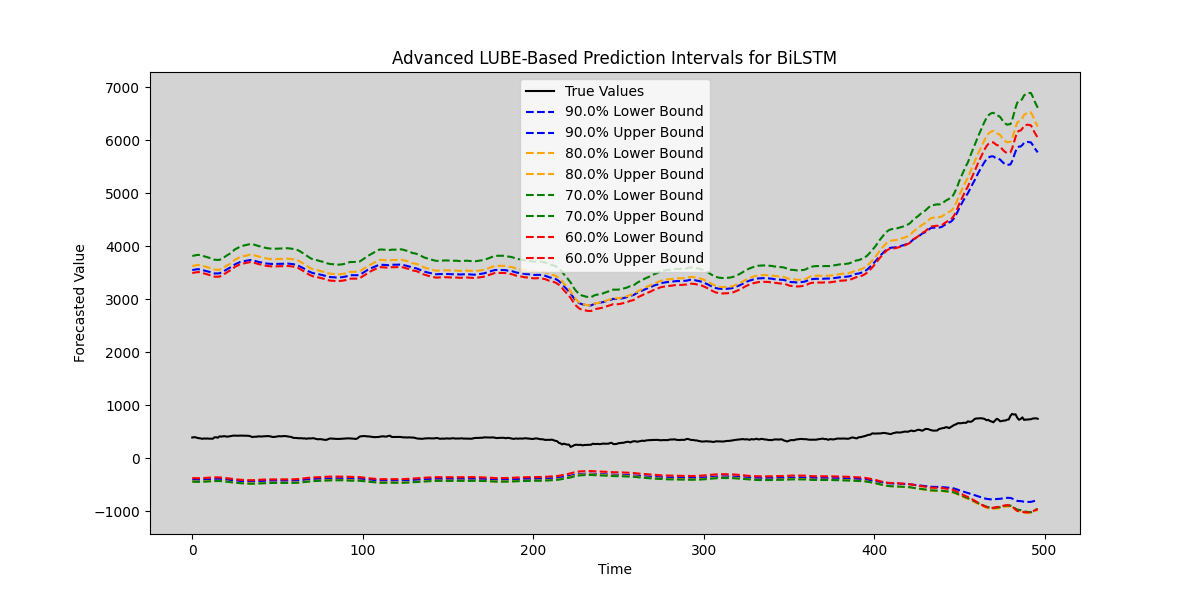
\includegraphics[width=\textwidth]{Chap02/figs/BiLSTM_advanced_lube_plot_ADANIPORTS.png}
                \caption{BiLSTM.}
            \end{subfigure}
            \hfill
            \begin{subfigure}[b]{\textwidth}
                \centering
                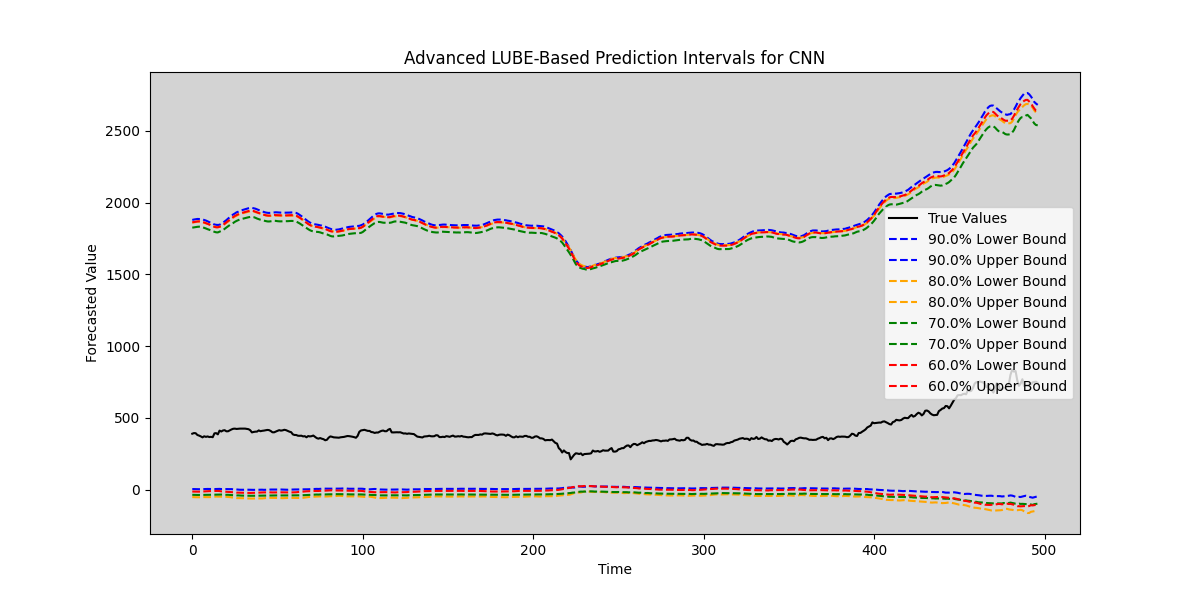
\includegraphics[width=\textwidth]{Chap02/figs/CNN_advanced_lube_plot_ADANIPORTS.png}
                \caption{CNN.}
            \end{subfigure}
            \begin{subfigure}[b]{\textwidth}
                \centering
                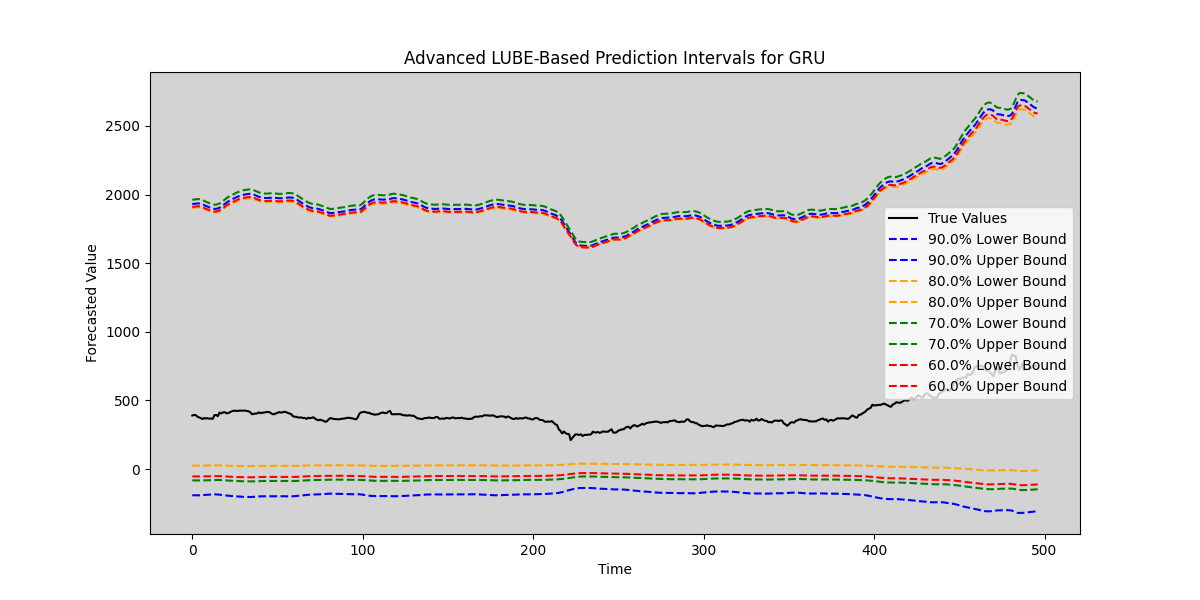
\includegraphics[width=\textwidth]{Chap02/figs/GRU_advanced_lube_plot_ADANIPORTS.png}
                \caption{GRU.}
            \end{subfigure}
            \begin{subfigure}[b]{\textwidth}
                \centering
                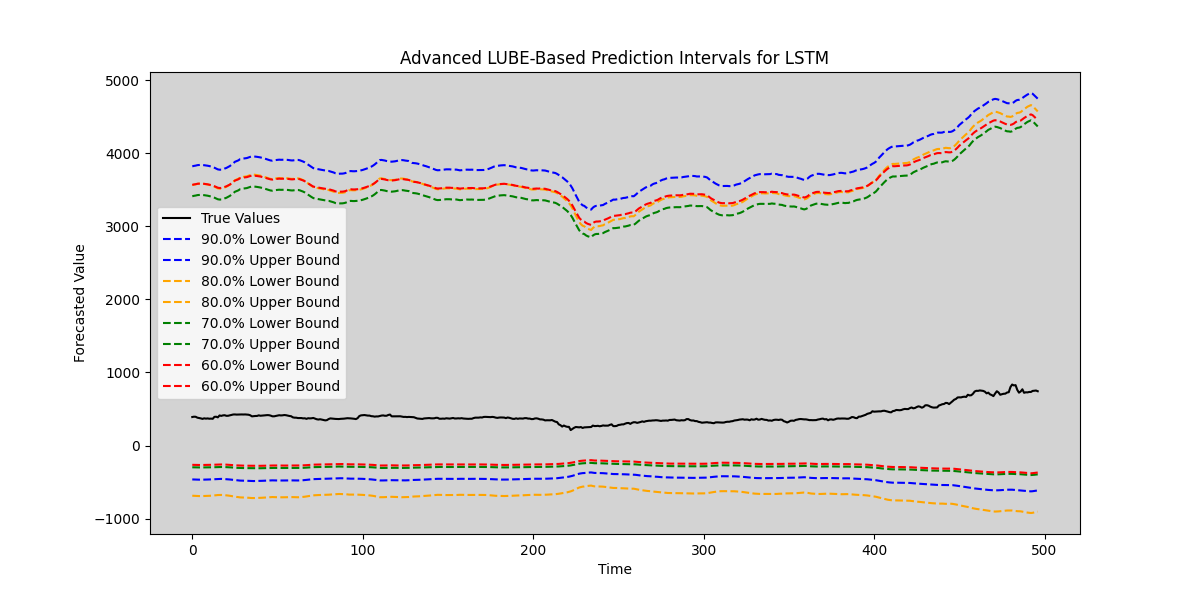
\includegraphics[width=\textwidth]{Chap02/figs/LSTM_advanced_lube_plot_ADANIPORTS.png}
                \caption{LSTM.}
            \end{subfigure}
        \end{minipage}
    
    \caption{Prediction Intervals for Adani Ports dataset obtained using Advanced LUBE method and (a) BiLSTM, (b) CNN, (c) GRU, (d) LSTM Models.}
    \label{Fi 3.2}
\end{figure}

Probabilistic forecasting methodologies have been tested on five disparate datasets: Adani Ports, Asian Paints, Axis Bank, Electricity Consumption Load, and Web Traffic. The six methodologies like Traditional LUBE, Advanced LUBE, QR-based, Bootstrap-based, Gaussian Distribution, and Weibull Distribution were used in all cases of these analyses. The performance was evaluated using the four critical metrics, which included Prediction Interval Coverage Probability (PICP), Prediction Interval Normalized Average Width (PINAW), Average Coverage Error (ACE), and Average Width Error (AWE). The following is a more detailed summary of the results and insights learned from the analysis of all five datasets:

\subsection{Performance Of Each Method Across Datasets}
The Traditional LUBE approach consistently achieved near-optimal PICP across all confidence levels and datasets, demonstrating reliable interval coverage. However, it generally produced wider prediction intervals, reflected in higher PINAW values—for instance, a PINAW of 10.01 at the 90\% confidence level with CNN DL model for the Adani Ports dataset \ref{Table 1}, indicating a highly conservative prediction. Similar trends were observed in the Asian Paints dataset, where the LSTM model showed a PINAW of 5.87 at 90\% confidence level. \ref{Table 2} Furthermore, across all datasets, the Traditional LUBE method exhibited higher AWE values compared to other methods, pointing to less efficient interval calibration. This trade-off suggests that while Traditional LUBE is dependable, it tends to produce overly cautious intervals, particularly in models like BiLSTM. In contrast, the Advanced LUBE method demonstrated superior performance across all datasets by generating narrower yet highly covered intervals. For example, in the Electricity Consumption dataset \ref{Table 4}, the GRU model achieved a PICP of 100\% with a significantly narrower PINAW of 1.35 at 90\% confidence level when compared to Traditional LUBE's 2.25. Similarly, in the Web Traffic dataset \ref{Table 5}, CNN attained a PINAW of 1.69 with a PICP of 99.19\% at 90\% confidence level. Additionally, the Advanced LUBE method consistently yielded lower ACE and AWE values, confirming its capability to deliver more dependable and efficient prediction intervals. The QR-based method, while producing the narrowest intervals among non-parametric approaches, often suffered from under-coverage. For instance, in the Axis Bank dataset at the 90\% confidence level, the BiLSTM model reached 96.65\% PICP with a very low PINAW of 0.15 \ref{Table 3}. Thus, despite its precision, the QR-based method falls short in applications requiring high reliability. The Bootstrap-based method held an intermediate location on interval coverage and width, with competitive PINAW and PICP values but not entirely on par with consistency of LUBE or Advanced LUBE. On the Adani Ports dataset, for example, the GRU model had a PICP of 68.43\% supported by a PINAW of 0.28 at 70\% confidence level which is a desirable output, while on the Electricity Consumption dataset, the GRU model held a PICP of only 28.20\% supported by a PINAW of 0.10 at 70\% confidence level \ref{Table 4} which is not at all desirable and shows major undercoverage. The Gaussian distribution method consistently produced the most narrow intervals but often failed to achieve the targeted PICP thresholds. On the Asian Paints dataset, for example, it had a PINAW of 0.42 at confidence level 70\% but a PICP of 83.58\%, supported by high ACE value of 13.58 indicating under coverage \ref{Table 6}. On the other hand, the Weibull distribution showed better PICP performance than Gaussian at 92.90\% at 90\% confidence on the Web Traffic dataset but at the cost of wider intervals (PINAW = 0.76) \ref{Table 10}.  Even though Weibull had better reliability, its relatively higher AWE values compared to Gaussian indicated lower efficiency and hence was better suited for application where coverage takes precedence over narrow intervals. Advanced LUBE hence proved to be the best overall and reliable methodology with high efficiency and reliability on a range of datasets and models. The Gaussian and Weibull Distribution Tables are shown in Tables \ref{Table 6} to \ref{Table 10}.

\subsection{Dataset Specific Observations}
The stock prices data for Adani Ports, Asian Paints and Axis Bank indicated consistent trends, with both the Traditional and Advanced LUBE methods indicating high PICP values. Fig \ref{Fi 3.2}, Fig. \ref{Fi 3.3} Significant differences, however, were observed among the widths of the intervals, with the Advanced LUBE technique showing a tendency to generate more tightened intervals. The QR-based and Bootstrap methods generated more efficient (narrow) intervals;Fig. \ref{Fi 3.3} Fig. \ref{Fi 3.4} however, these came at the cost of reliability as the coverage levels were lower. The data for Electricity Consumption Load indicated the applicability and efficiency of the Advanced LUBE methodology, which obtained high coverage along with efficient interval lengths, while the QR-based and Bootstrap methods indicated poor performance with very low PICP values. A similar trend was also observed for the Web Traffic dataset, where both the Advanced LUBE and Bootstrap methods indicated relatively higher effectiveness by balancing coverage and interval widths.

\subsection{Recommendations}
The Advanced LUBE method is best suited for applications that demand high reliability alongside efficient interval widths as it consistently outperformed other approaches across all datasets and evaluation metrics. The Bootstrap-based method serves well in scenarios where a moderate level of reliability is acceptable, offering a balanced trade-off between coverage and interval width. Among the parametric methods, the Gaussian approach yields very narrow and precise intervals but suffers from under-coverage, making it less reliable Fig. \ref{Fi 3.6}. In contrast, the Weibull distribution delivers better coverage but tends to produce wider intervals, reducing its efficiency for applications requiring tightly bound predictions Fig. \ref{Fi 3.7}.

\begin{figure}[H]
    \centering
        \begin{minipage}{0.6\textwidth}
            \centering
            \begin{subfigure}[b]{1.0\textwidth}
                \centering
                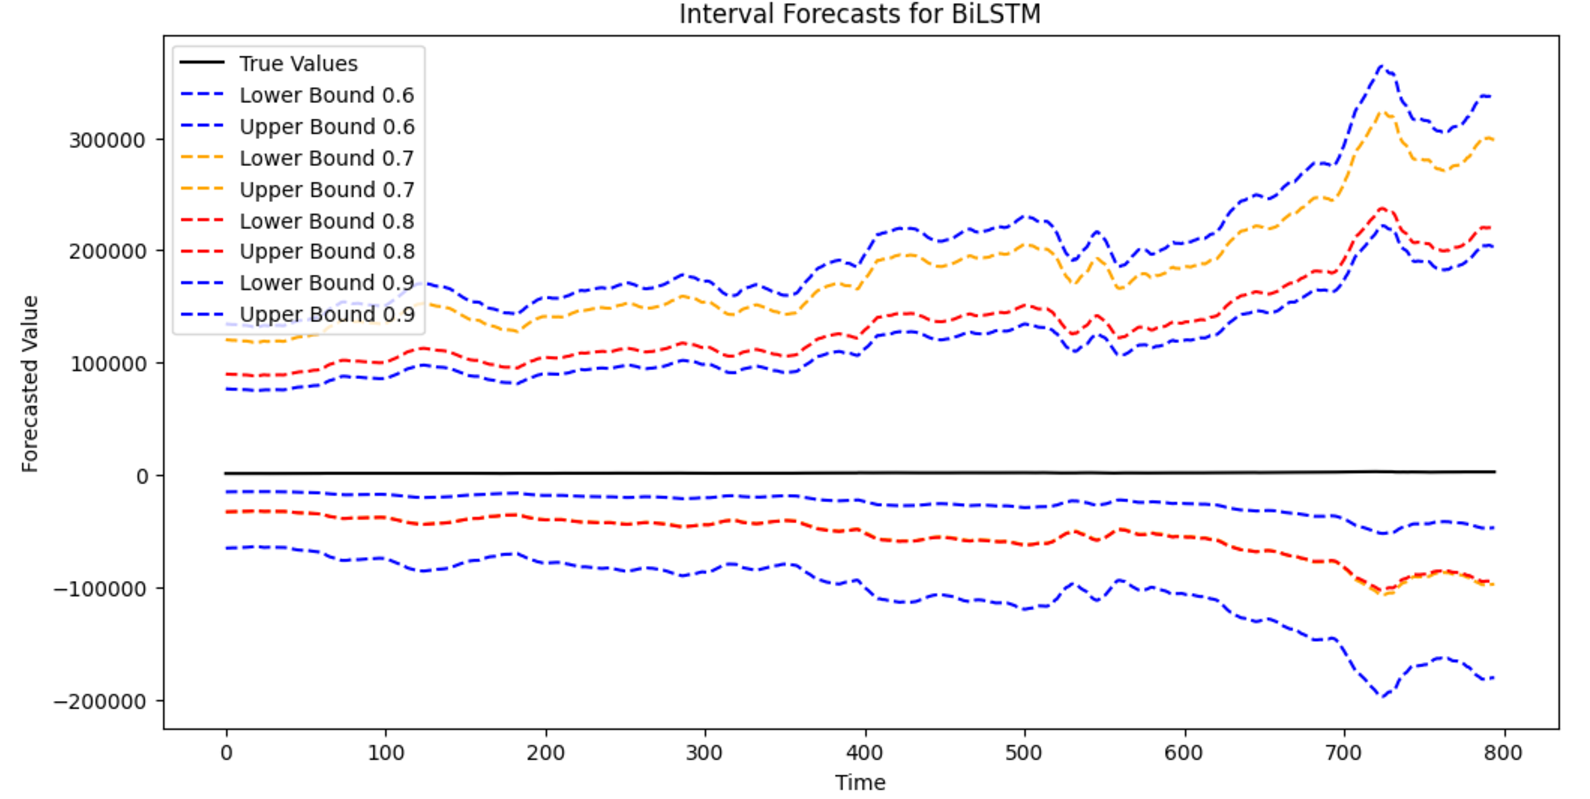
\includegraphics[width=\textwidth]{Chap02/figs/LUBE_BiLSTM_AsianPaints.png}
                \caption{BiLSTM.}
            \end{subfigure}
            \hfill
            \begin{subfigure}[b]{1.0\textwidth}
                \centering
                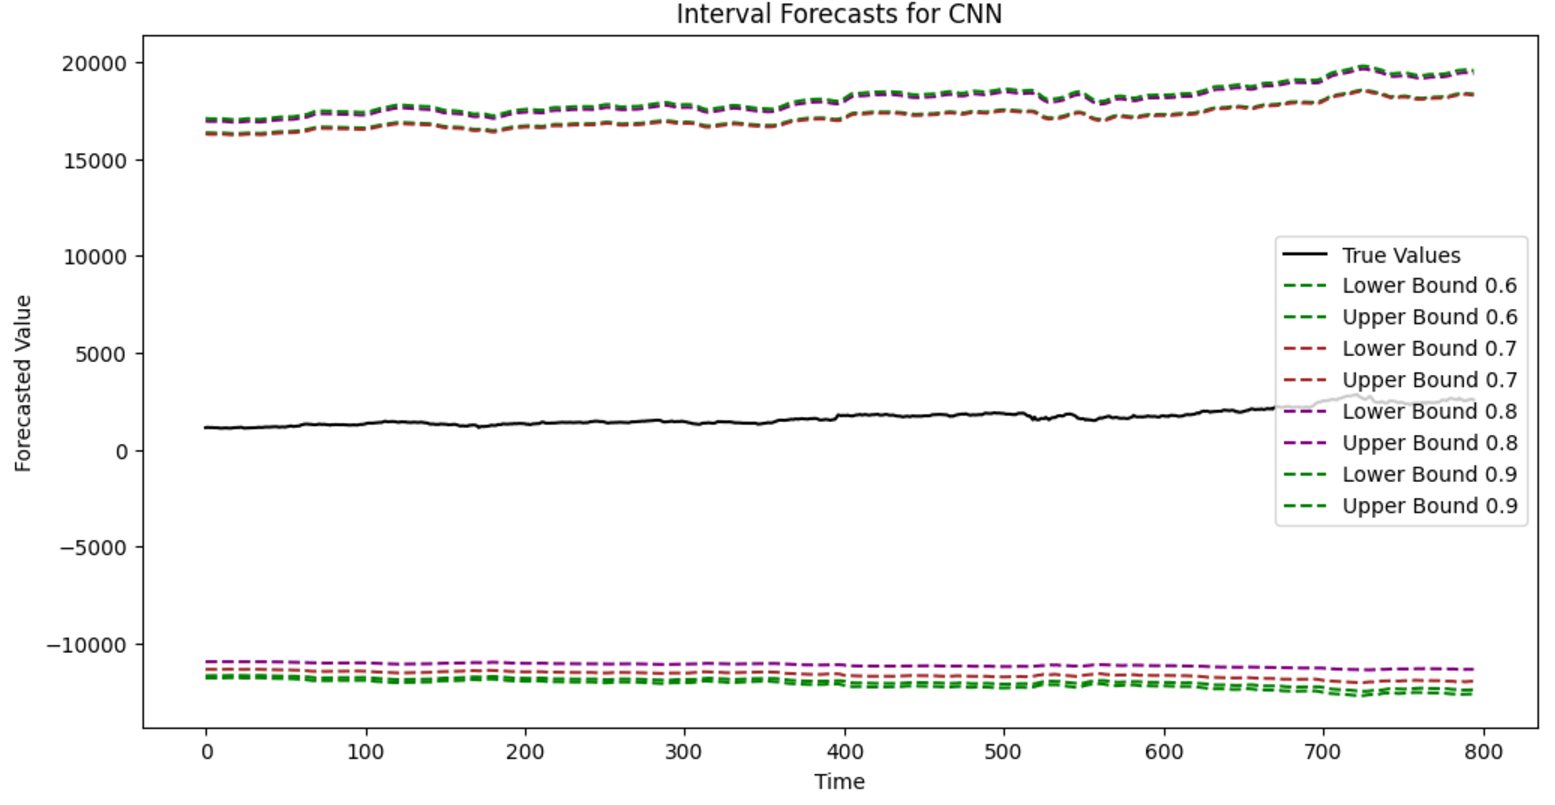
\includegraphics[width=\textwidth]{Chap02/figs/LUBE_CNN_AsianPaints.png}
                \caption{CNN.}
            \end{subfigure}
            \begin{subfigure}[b]{1.0\textwidth}
                \centering
                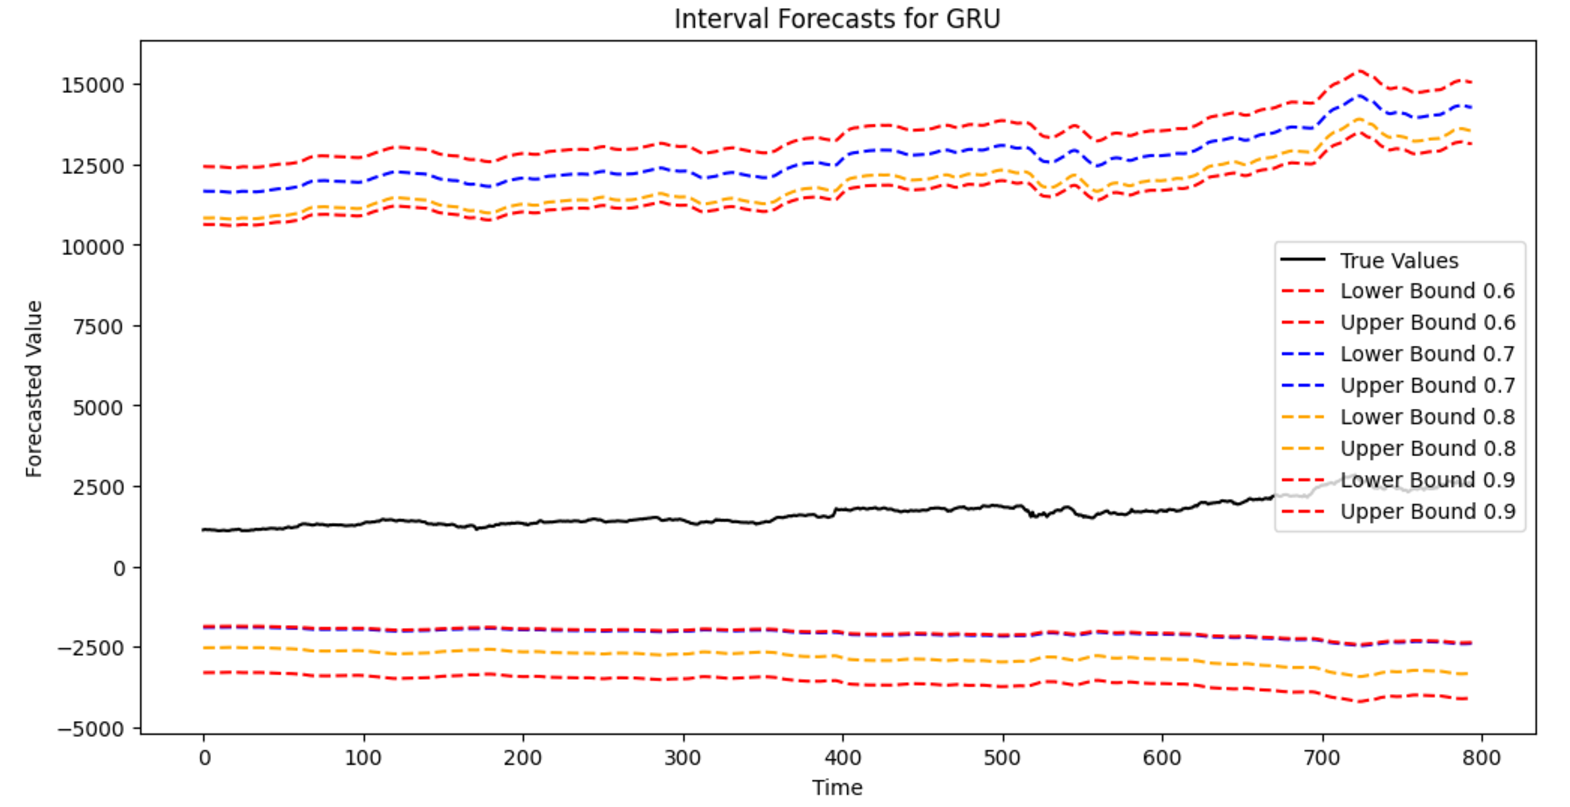
\includegraphics[width=\textwidth]{Chap02/figs/LUBE_GRU_AsianPaints.png}
                \caption{GRU.}
            \end{subfigure}
            \begin{subfigure}[b]{1.0\textwidth}
                \centering
                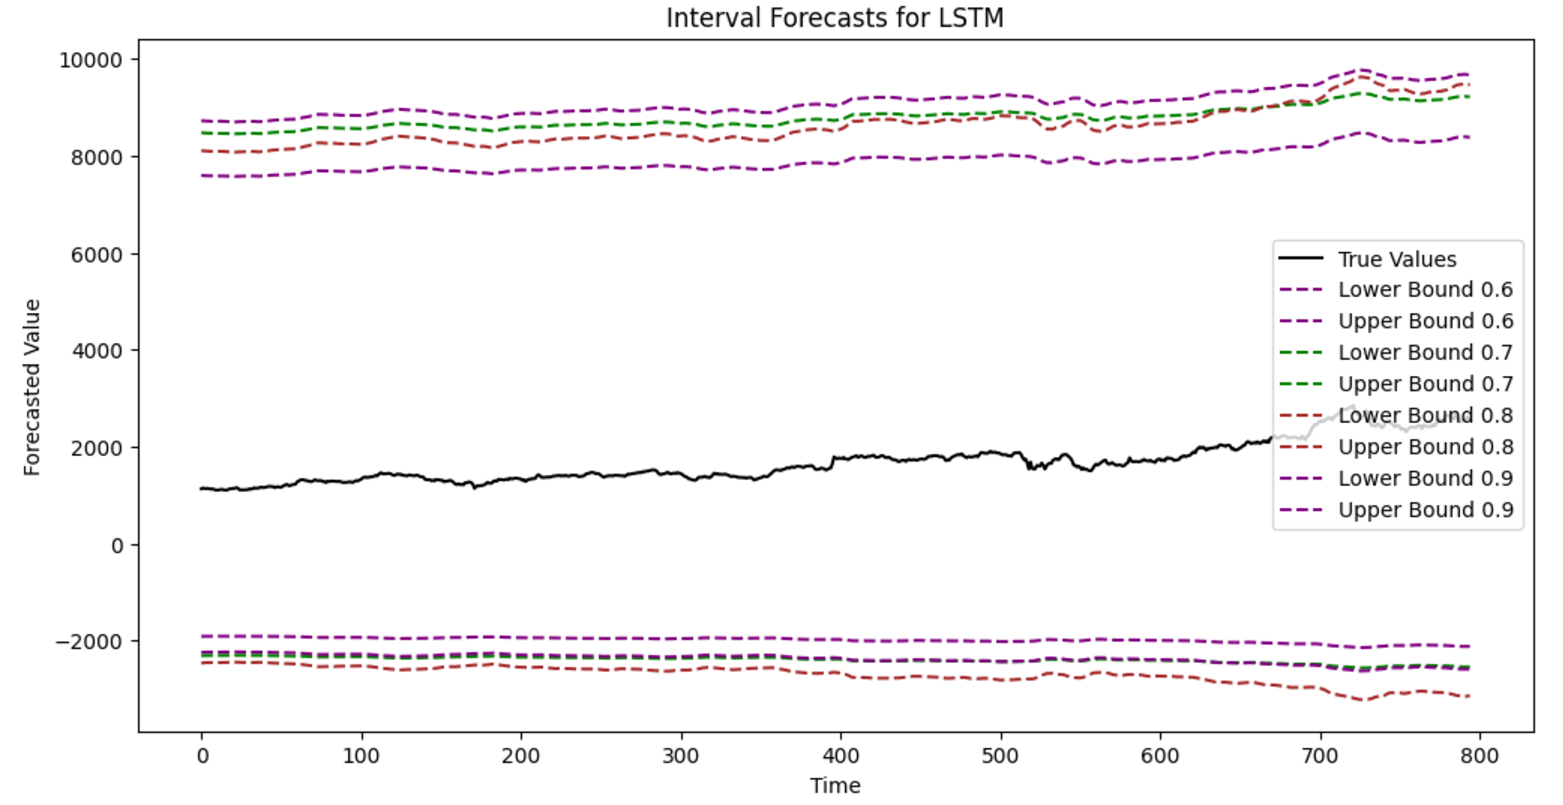
\includegraphics[width=\textwidth]{Chap02/figs/LUBE_LSTM_AsianPaints.png}
                \caption{LSTM.}
            \end{subfigure}
        \end{minipage}
    
    \caption{Prediction Intervals for Asian Paints dataset obtained using Traditional LUBE method and (a) BiLSTM, (b) CNN, (c) GRU, (d) LSTM Models.}
    \label{Fi 3.3}
\end{figure}

\begin{figure}[H]
    \centering
        \begin{minipage}{0.6\textwidth}
            \centering
            \begin{subfigure}[b]{1.0\textwidth}
                \centering
                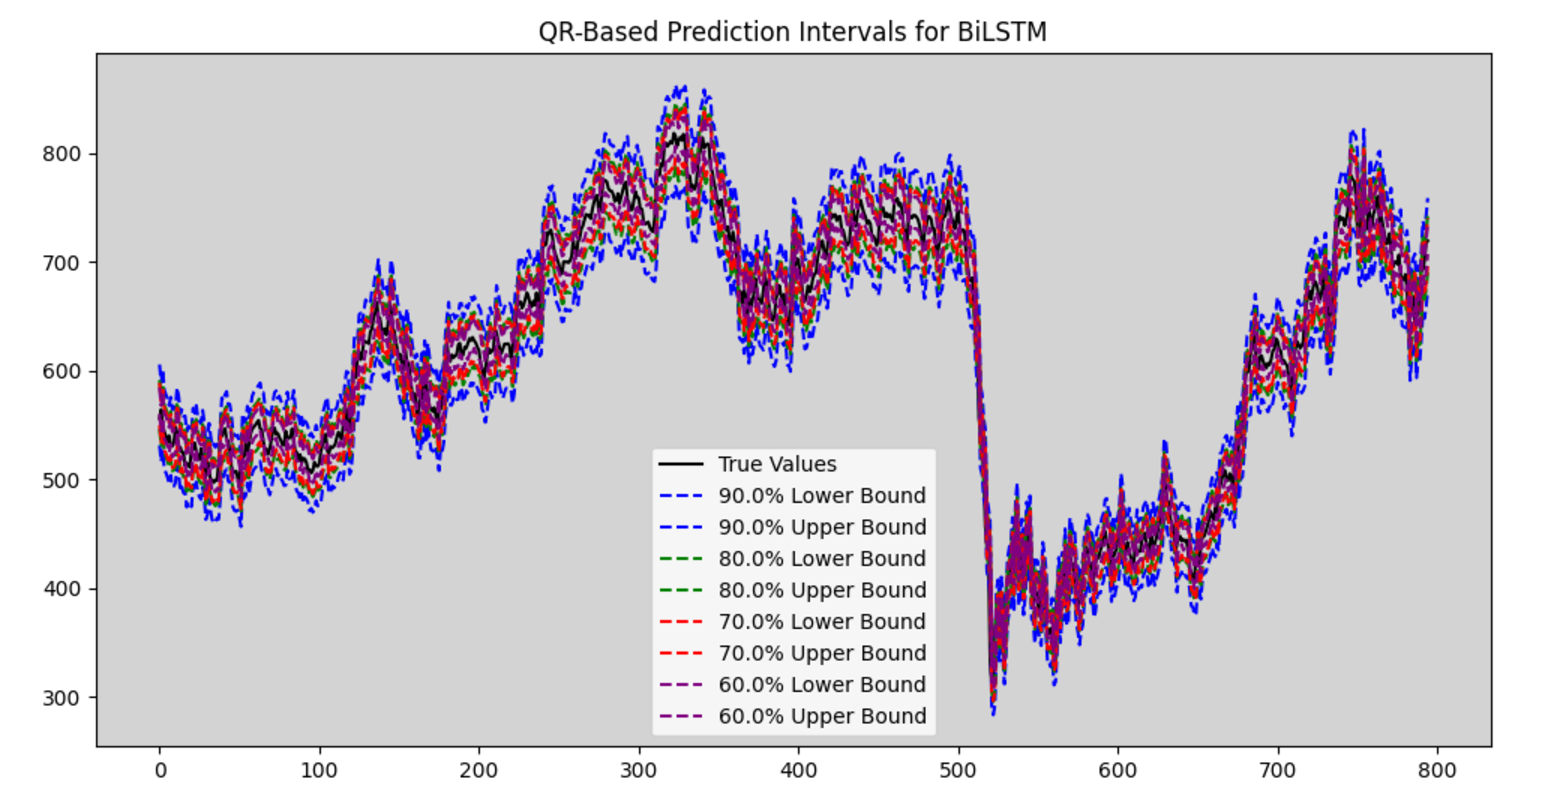
\includegraphics[width=\textwidth]{Chap02/figs/QR_BiLSTM_AxisBank_Original.png}
                \caption{BiLSTM.}
            \end{subfigure}
            \hfill
            \begin{subfigure}[b]{1.0\textwidth}
                \centering
                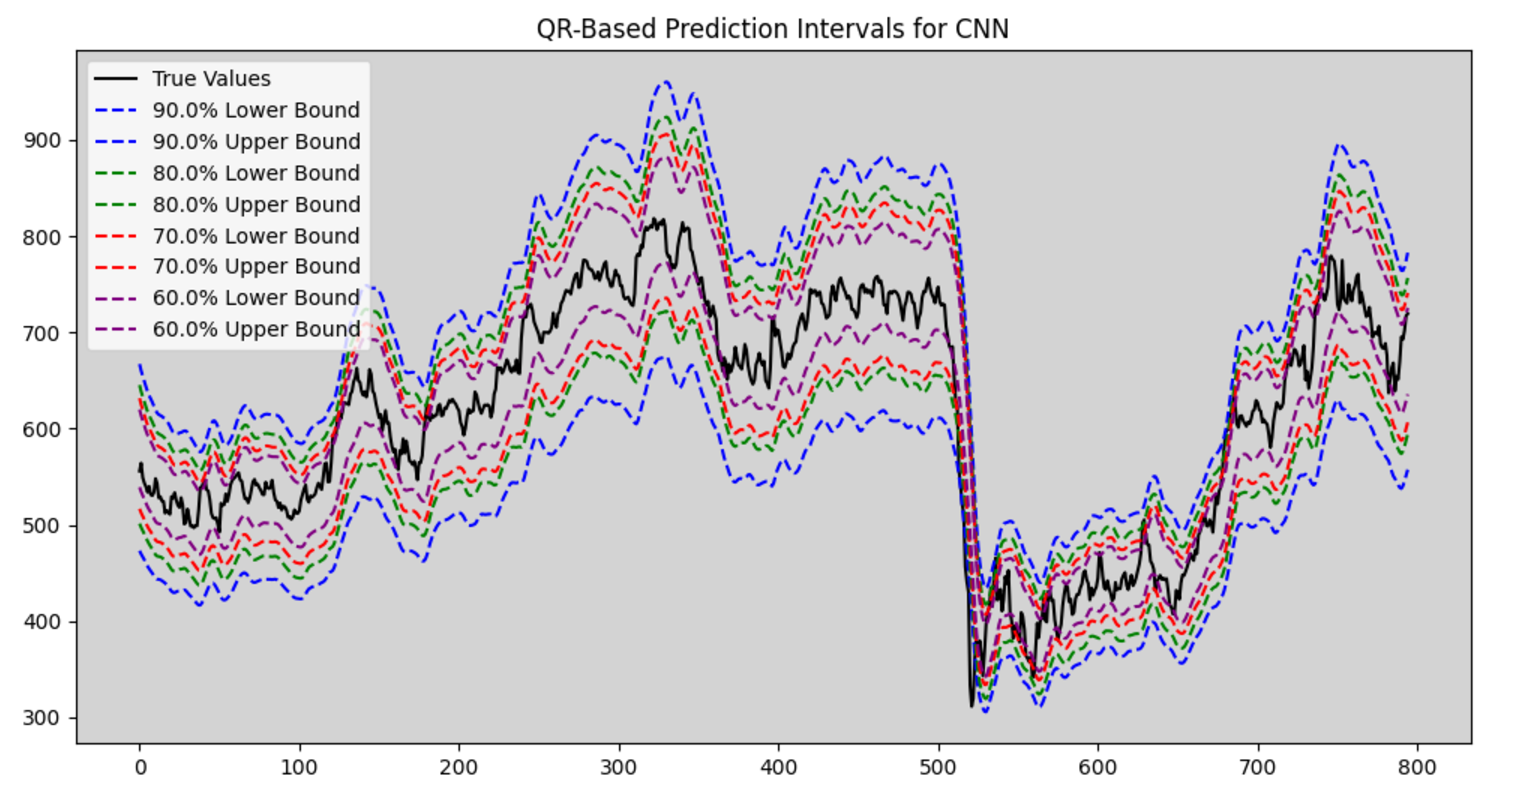
\includegraphics[width=\textwidth]{Chap02/figs/QR_CNN_AxisBank.png}
                \caption{CNN.}
            \end{subfigure}
            \begin{subfigure}[b]{1.0\textwidth}
                \centering
                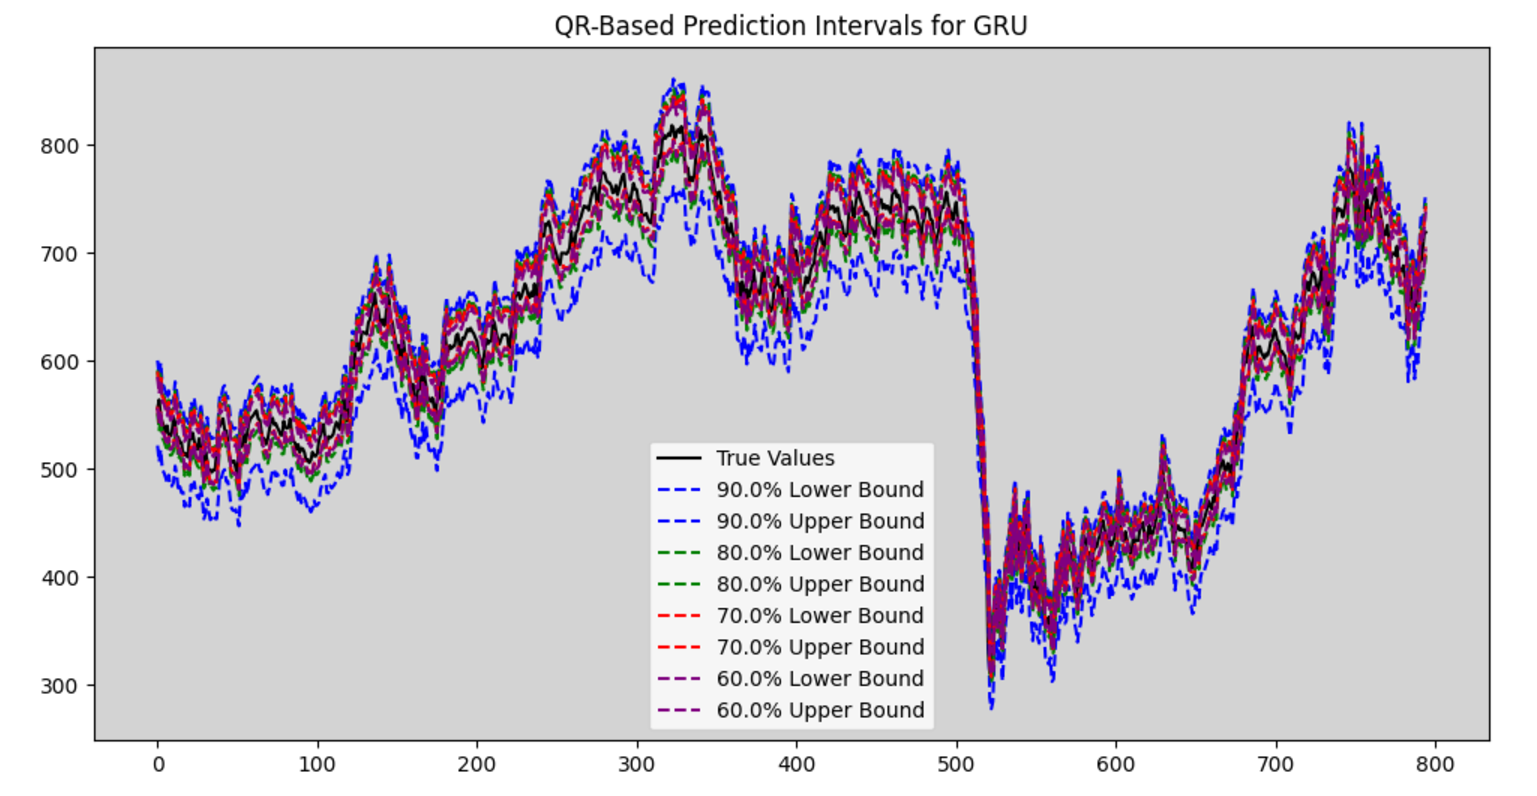
\includegraphics[width=\textwidth]{Chap02/figs/QR_GRU_AxisBank.png}
                \caption{GRU.}
            \end{subfigure}
            \begin{subfigure}[b]{1.0\textwidth}
                \centering
                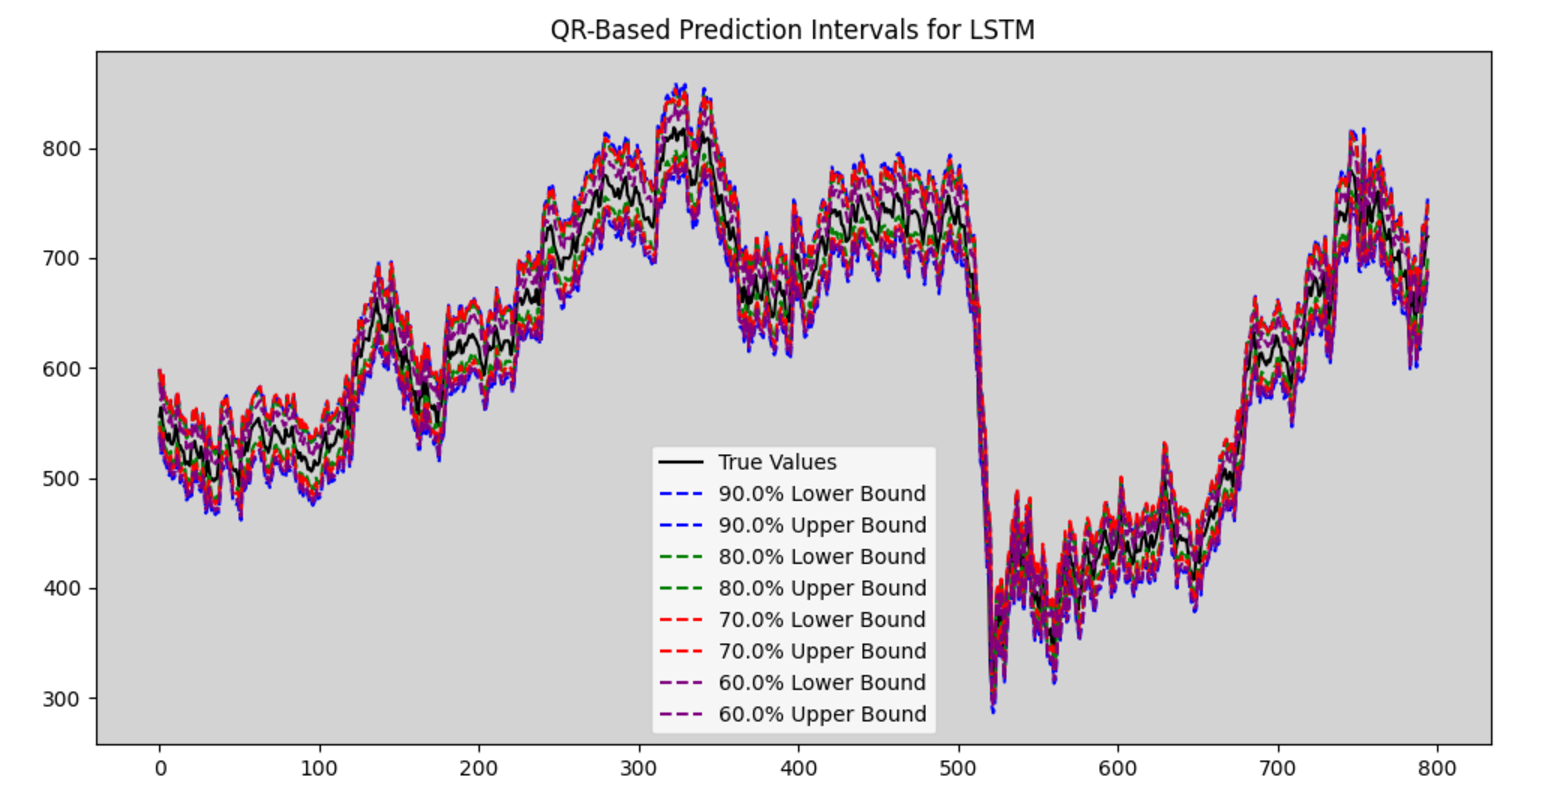
\includegraphics[width=\textwidth]{Chap02/figs/QR_LSTM_AxisBank.png}
                \caption{LSTM.}
            \end{subfigure}
        \end{minipage}
    
    \caption{Prediction Intervals for Axis Bank dataset obtained using QR-based method and (a) BiLSTM, (b) CNN, (c) GRU, (d) LSTM Models.}
    \label{Fi 3.4}
\end{figure}

\begin{figure}[H]
    \centering
        \begin{minipage}{0.6\textwidth}
            \centering
            \begin{subfigure}[b]{1.0\textwidth}
                \centering
                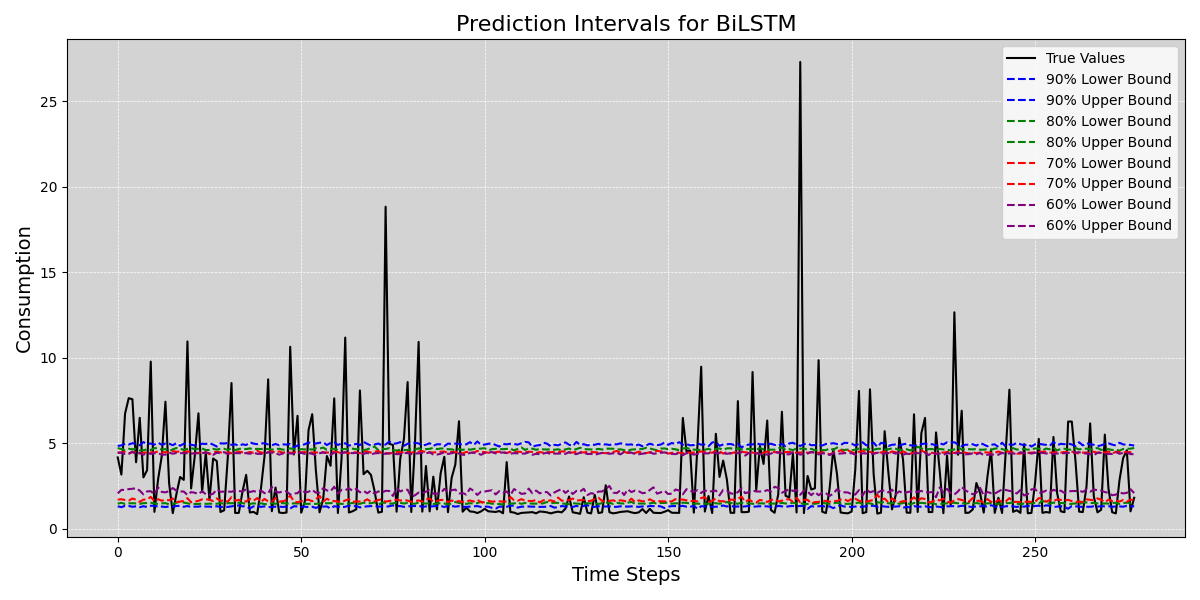
\includegraphics[width=\textwidth]{Chap02/figs/Prediction_Intervals_Styled_BiLSTM_Electricity_Consumption.png}
                \caption{BiLSTM.}
            \end{subfigure}
            \hfill
            \begin{subfigure}[b]{1.0\textwidth}
                \centering
                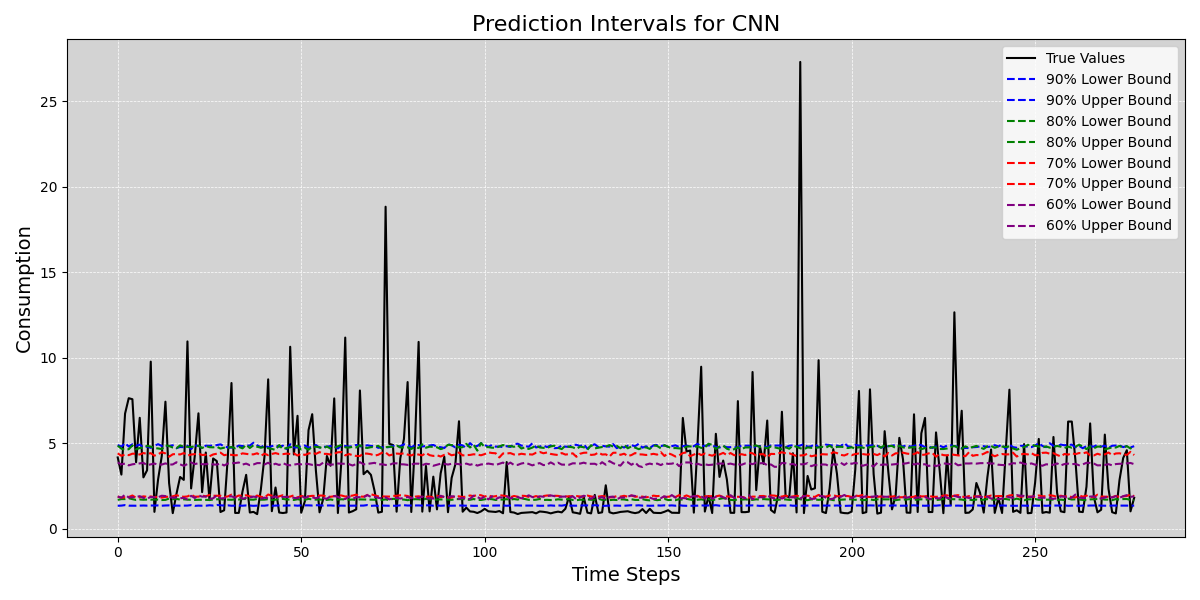
\includegraphics[width=\textwidth]{Chap02/figs/Prediction_Intervals_Styled_CNN_Electricity_Consumption.png}
                \caption{CNN.}
            \end{subfigure}
            \begin{subfigure}[b]{1.0\textwidth}
                \centering
                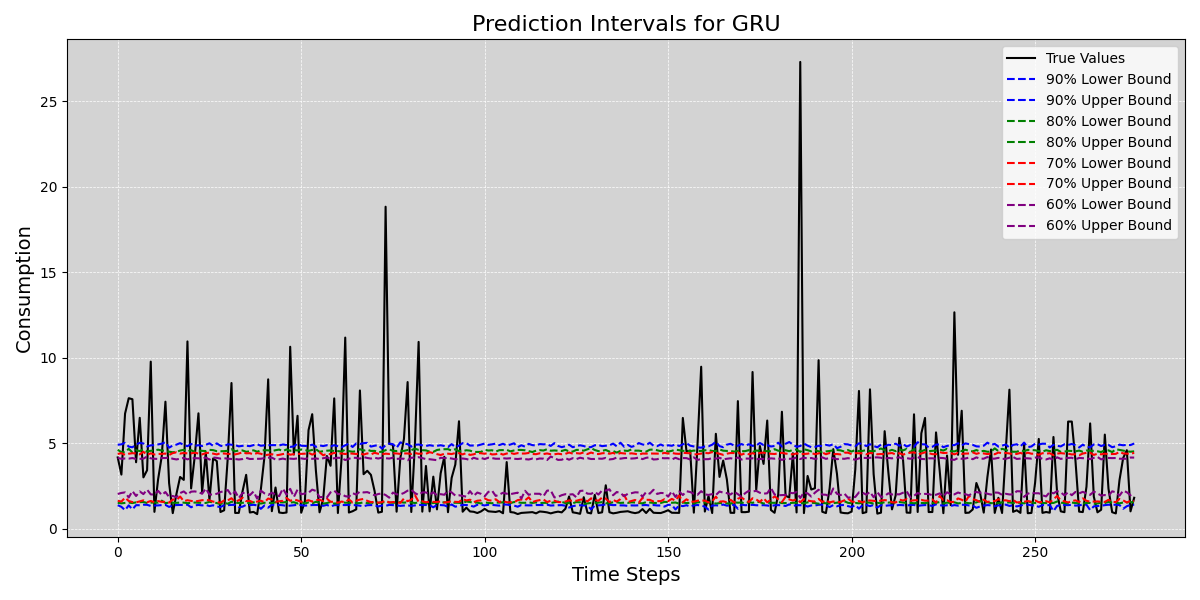
\includegraphics[width=\textwidth]{Chap02/figs/Prediction_Intervals_Styled_GRU_Electricity_Consumption.png}
                \caption{GRU.}
            \end{subfigure}
            \begin{subfigure}[b]{1.0\textwidth}
                \centering
                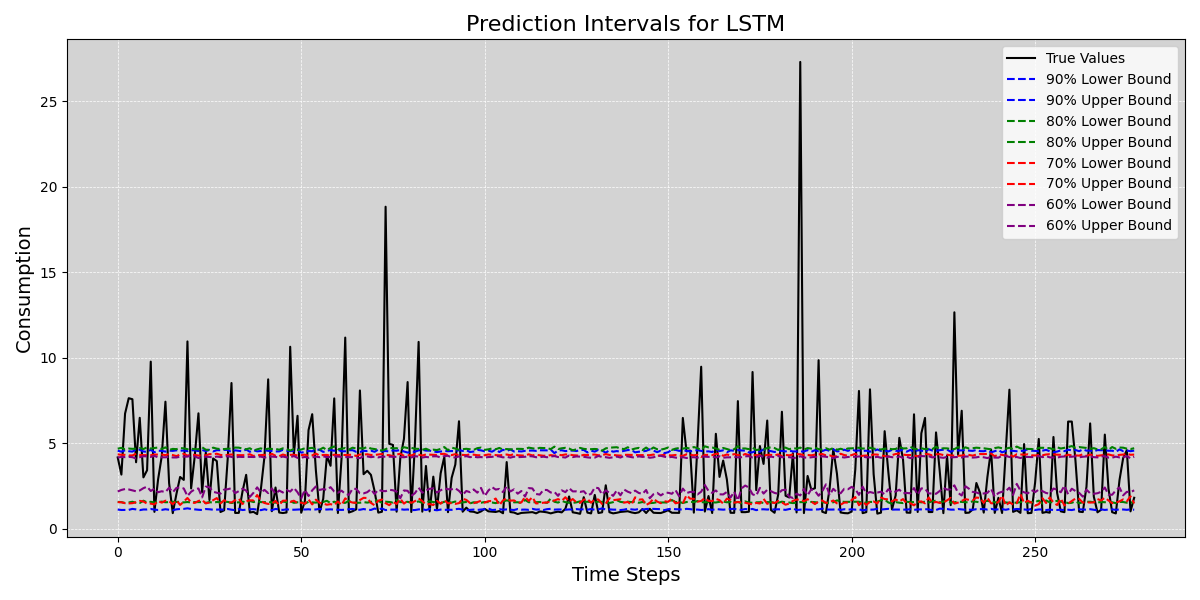
\includegraphics[width=\textwidth]{Chap02/figs/Prediction_Intervals_Styled_LSTM_Electricity_Consumption.png}
                \caption{LSTM.}
            \end{subfigure}
        \end{minipage}
    
    \caption{Prediction Intervals for Electricity Consumption dataset obtained using Bootstrap-based method and (a) BiLSTM, (b) CNN, (c) GRU, (d) LSTM Models.}
    \label{Fi 3.5}
\end{figure}

\begin{figure}[H]
    \centering
        \begin{minipage}{0.6\textwidth}
            \centering
            \begin{subfigure}[b]{0.8\textwidth}
                \centering
                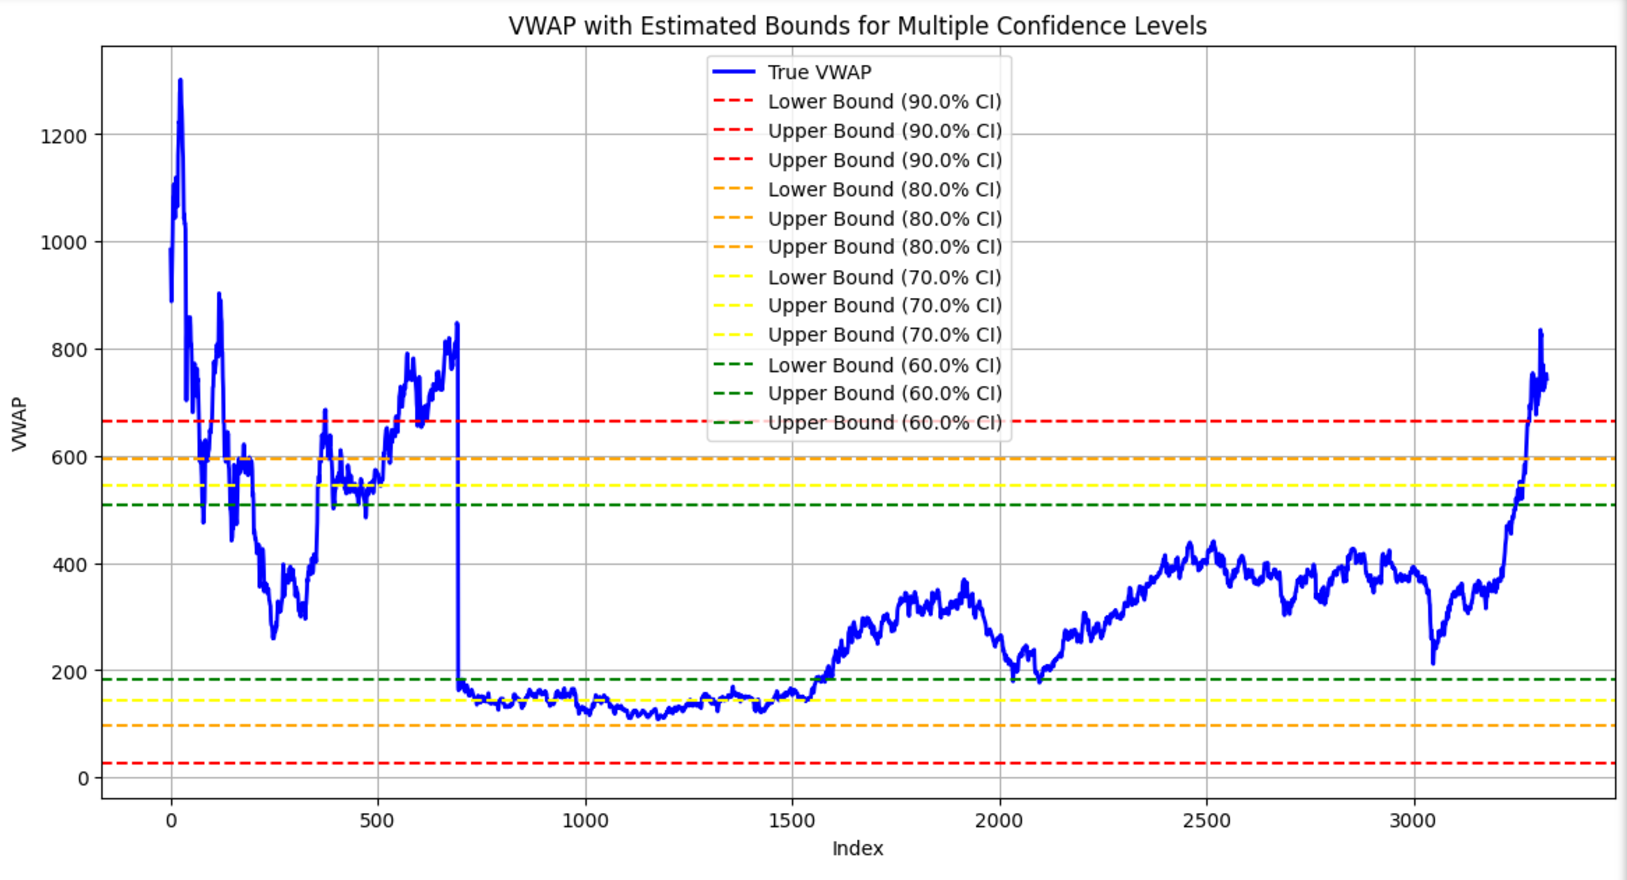
\includegraphics[width=\textwidth]{Chap02/figs/Gaussian_AdaniPorts.png}
                \caption{Adani Ports Dataset.}
            \end{subfigure}
            \hfill
            \begin{subfigure}[b]{0.8\textwidth}
                \centering
                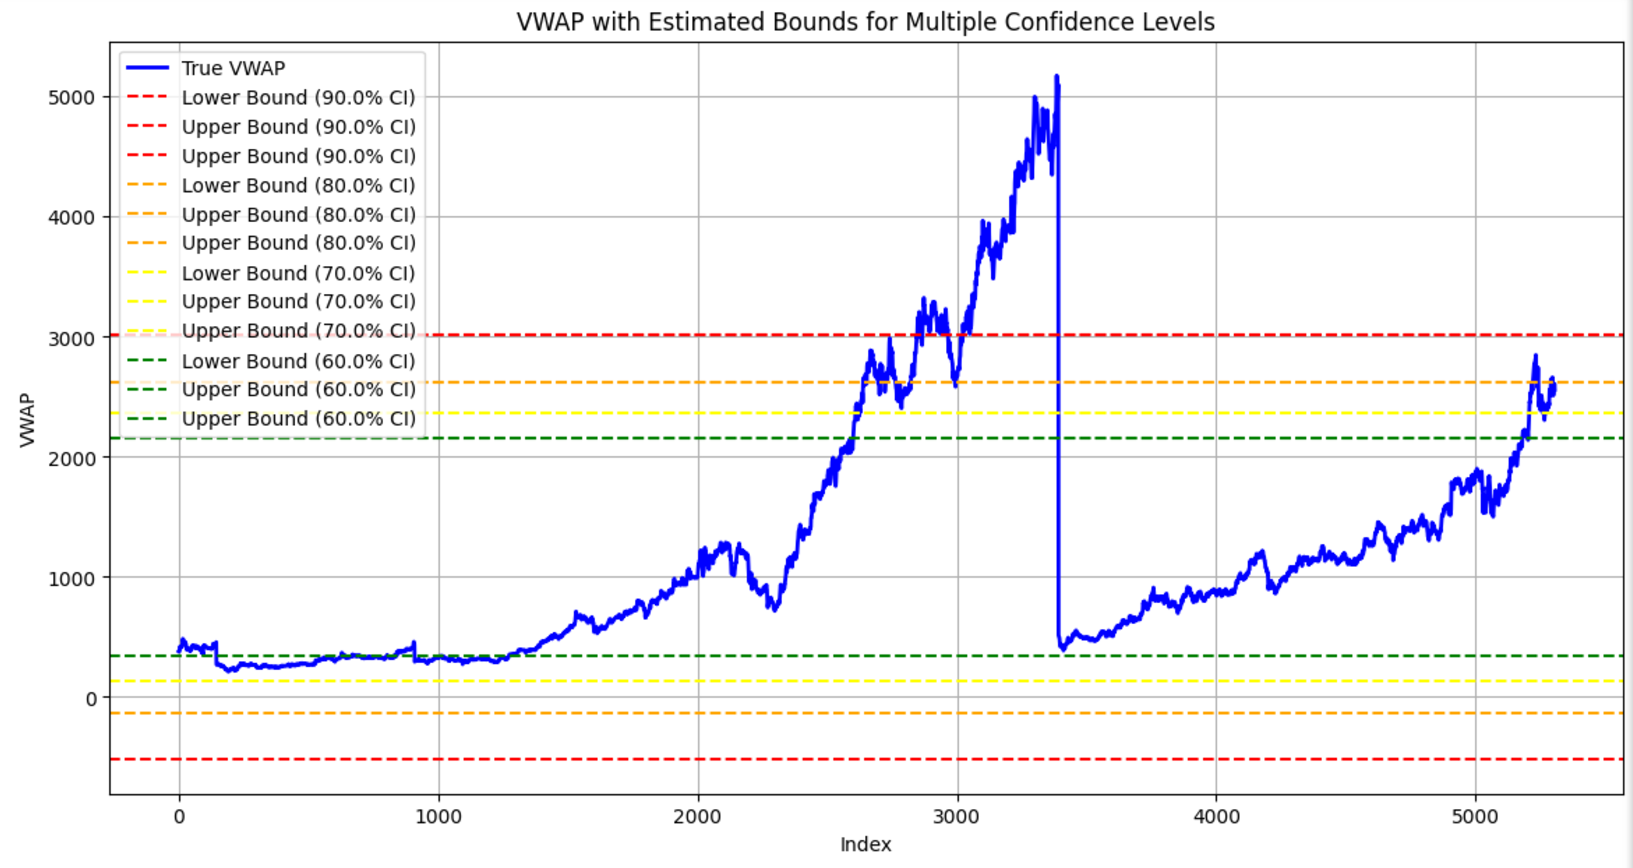
\includegraphics[width=\textwidth]{Chap02/figs/Gaussian_AsianPaints.png}
                \caption{Asian Paints Dataset.}
            \end{subfigure}
            \begin{subfigure}[b]{0.8\textwidth}
                \centering
                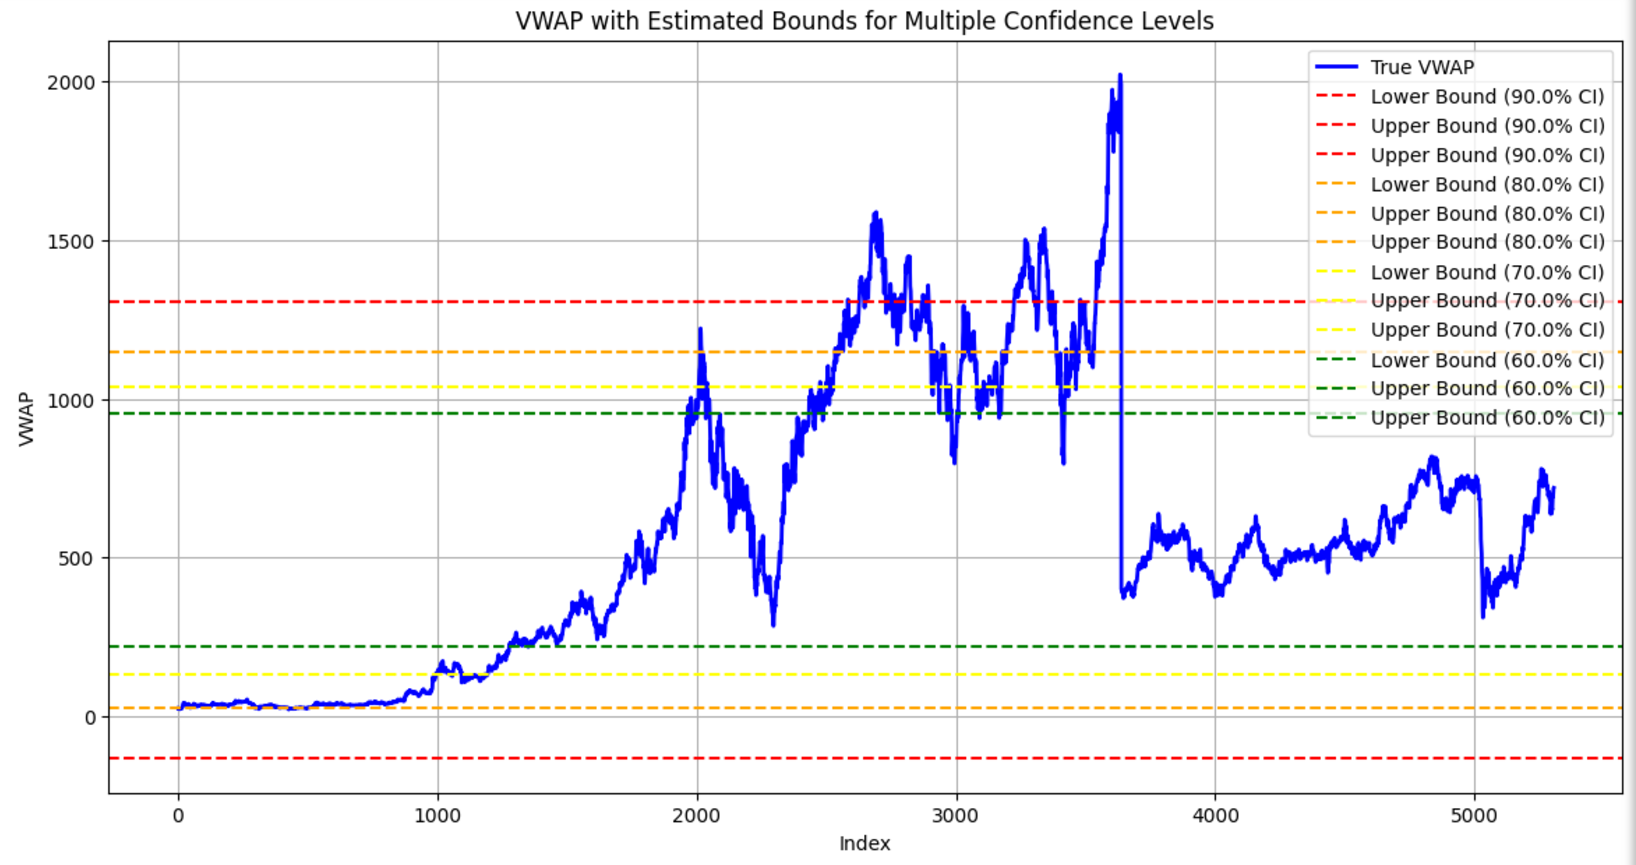
\includegraphics[width=\textwidth]{Chap02/figs/Gaussian_AxisBank.png}
                \caption{Axis Bank Dataset.}
            \end{subfigure}
            \begin{subfigure}[b]{0.8\textwidth}
                \centering
                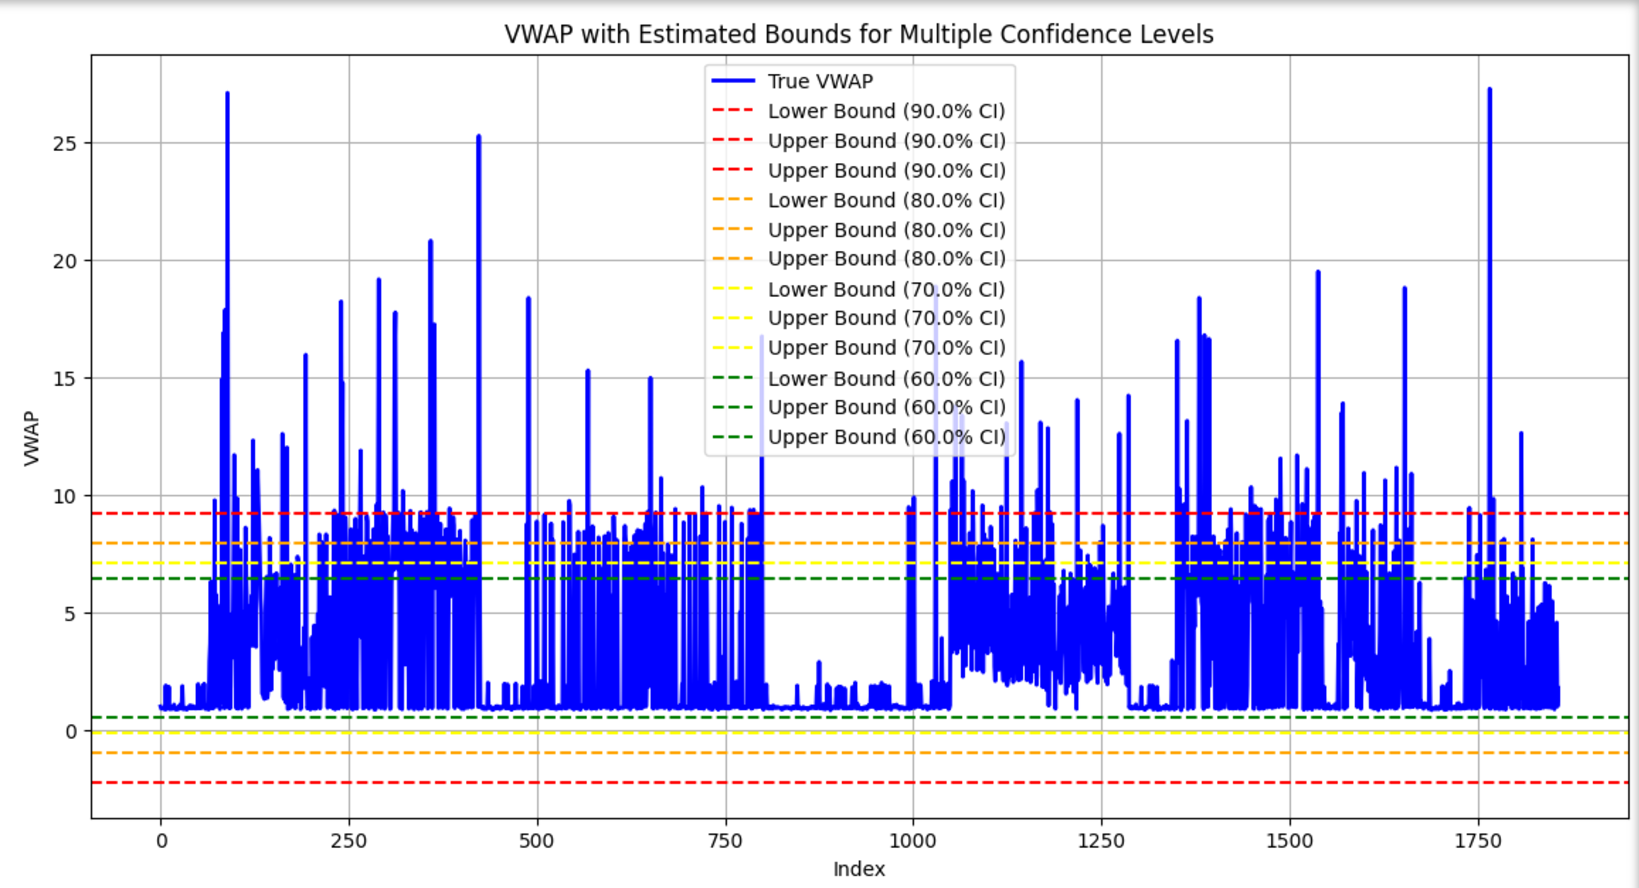
\includegraphics[width=\textwidth]{Chap02/figs/Gaussian_Electricity_Consumption.png}
                \caption{Electricity Consumption Dataset.}
            \end{subfigure}

            \begin{subfigure}[b]{0.8\textwidth}
                \centering
                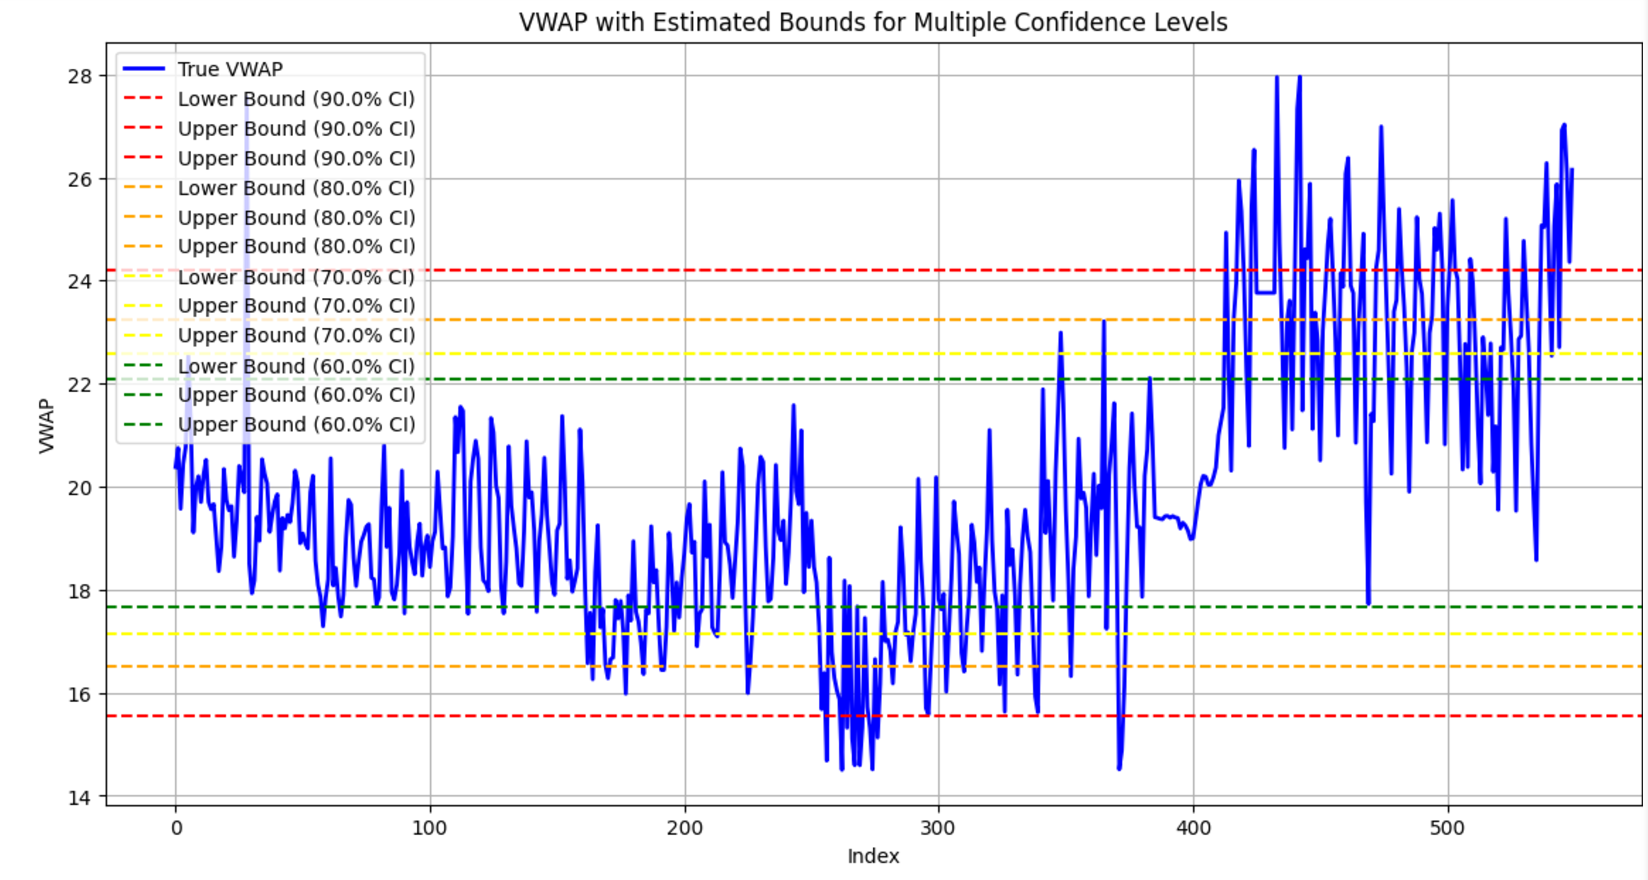
\includegraphics[width=\textwidth]{Chap02/figs/Gaussian_Web_Traffic.png}
                \caption{Web Traffic Dataset.}
            \end{subfigure}
        \end{minipage}
    
    \caption{Prediction Intervals for (a) Adani Ports, (b) Asian Paints, (c) Axis Bank, (d) Electricity Consumption Load, (e) Web Traffic datasets obtained using Gaussian Distribution method.}
    \label{Fi 3.6}
\end{figure}

\begin{figure}[H]
    \centering
        \begin{minipage}{0.6\textwidth}
            \centering
            \begin{subfigure}[b]{0.8\textwidth}
                \centering
                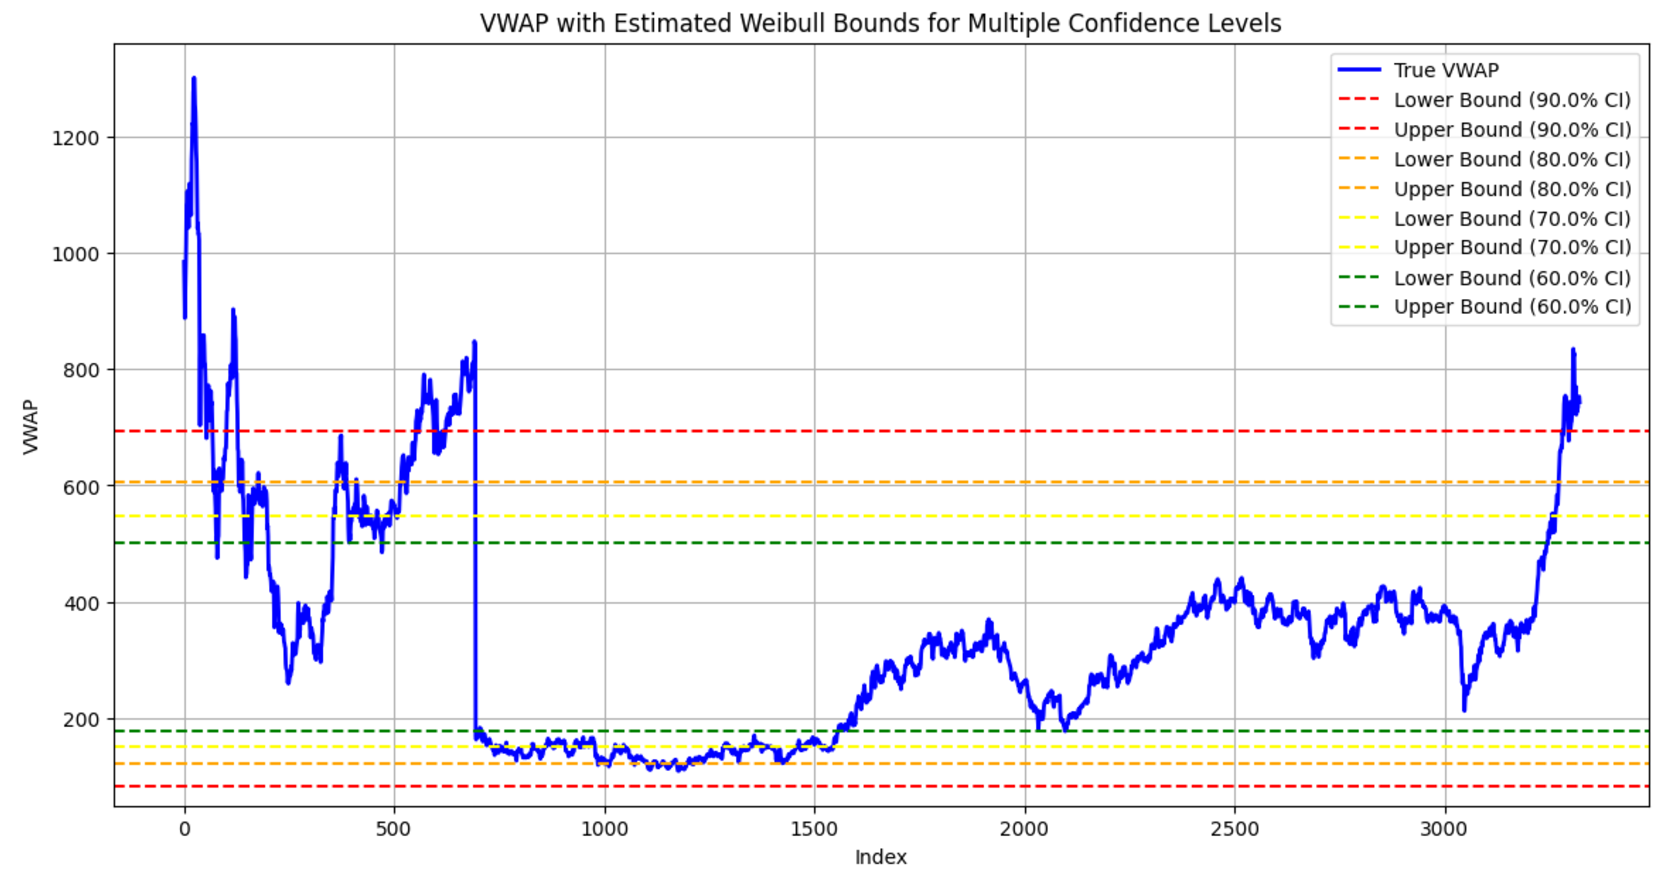
\includegraphics[width=\textwidth]{Chap02/figs/Weibull_AdaniPorts.png}
                \caption{Adani Ports Dataset.}
            \end{subfigure}
            \hfill
            \begin{subfigure}[b]{0.8\textwidth}
                \centering
                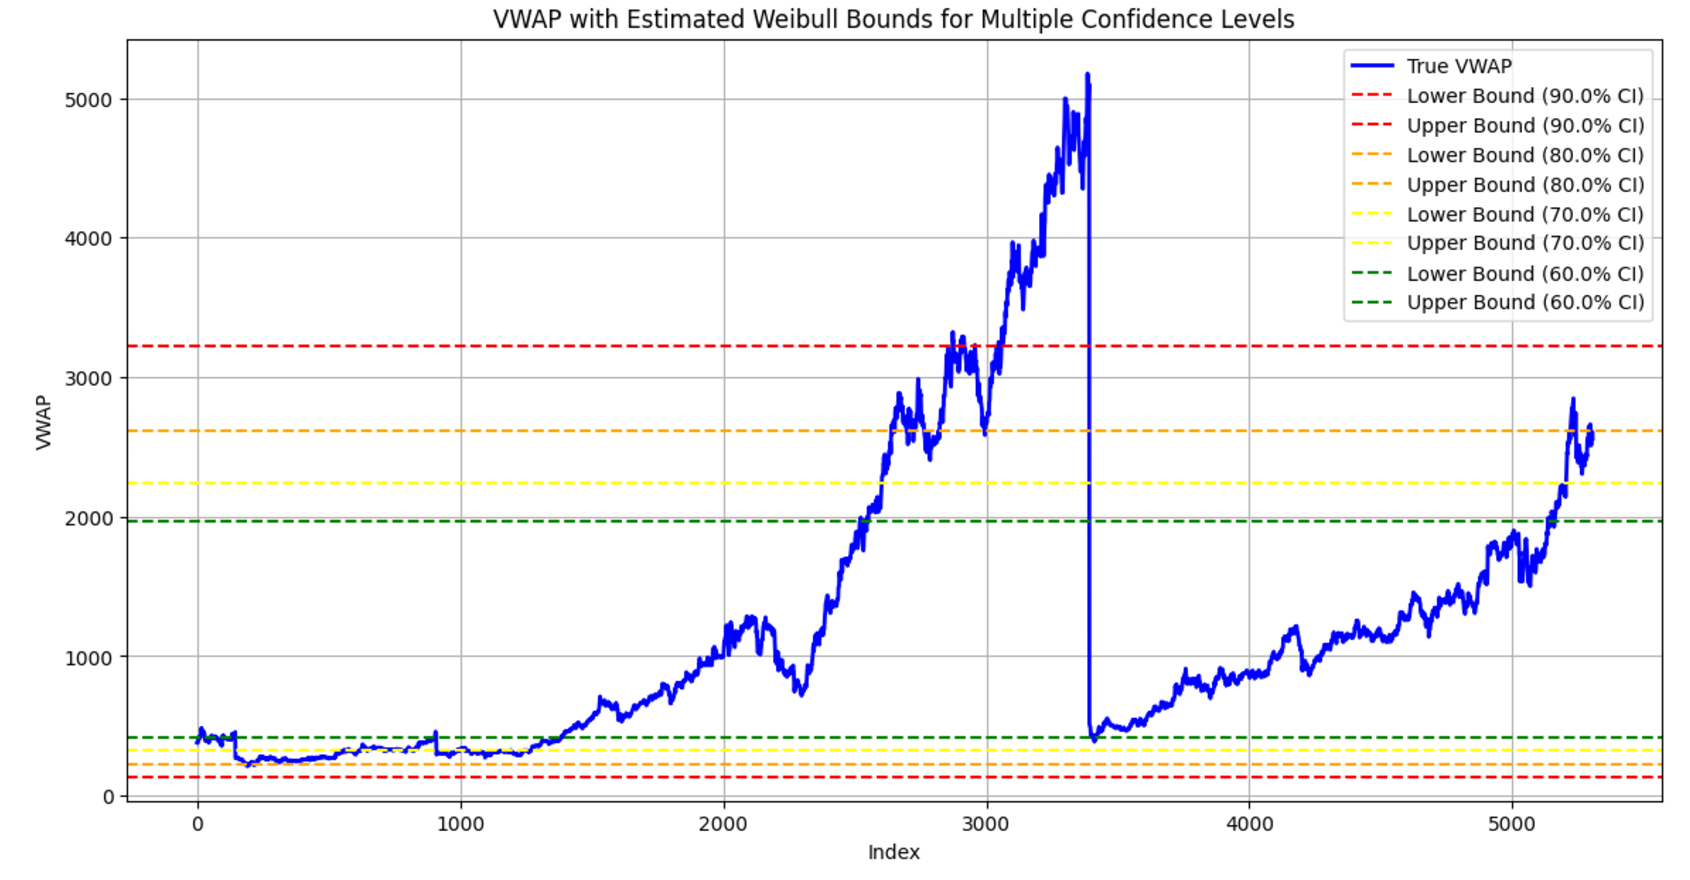
\includegraphics[width=\textwidth]{Chap02/figs/Weibull_AsianPaints.png}
                \caption{Asian Paints Dataset.}
            \end{subfigure}
            \begin{subfigure}[b]{0.8\textwidth}
                \centering
                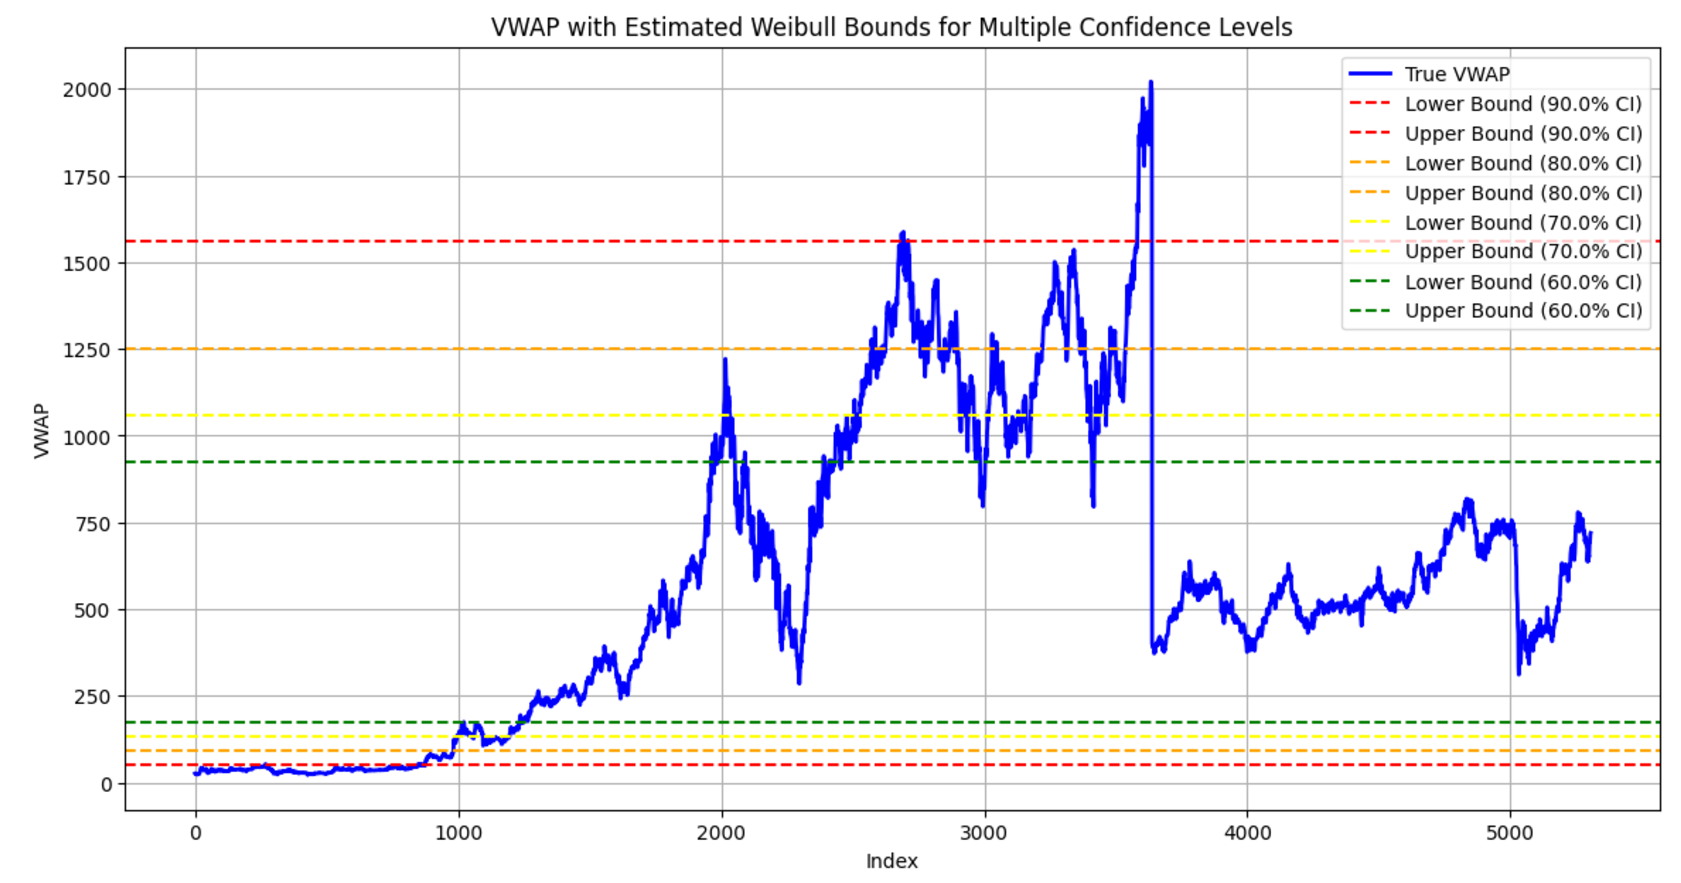
\includegraphics[width=\textwidth]{Chap02/figs/Weibull_AxisBank.png}
                \caption{Axis Bank Dataset.}
            \end{subfigure}
            \begin{subfigure}[b]{0.8\textwidth}
                \centering
                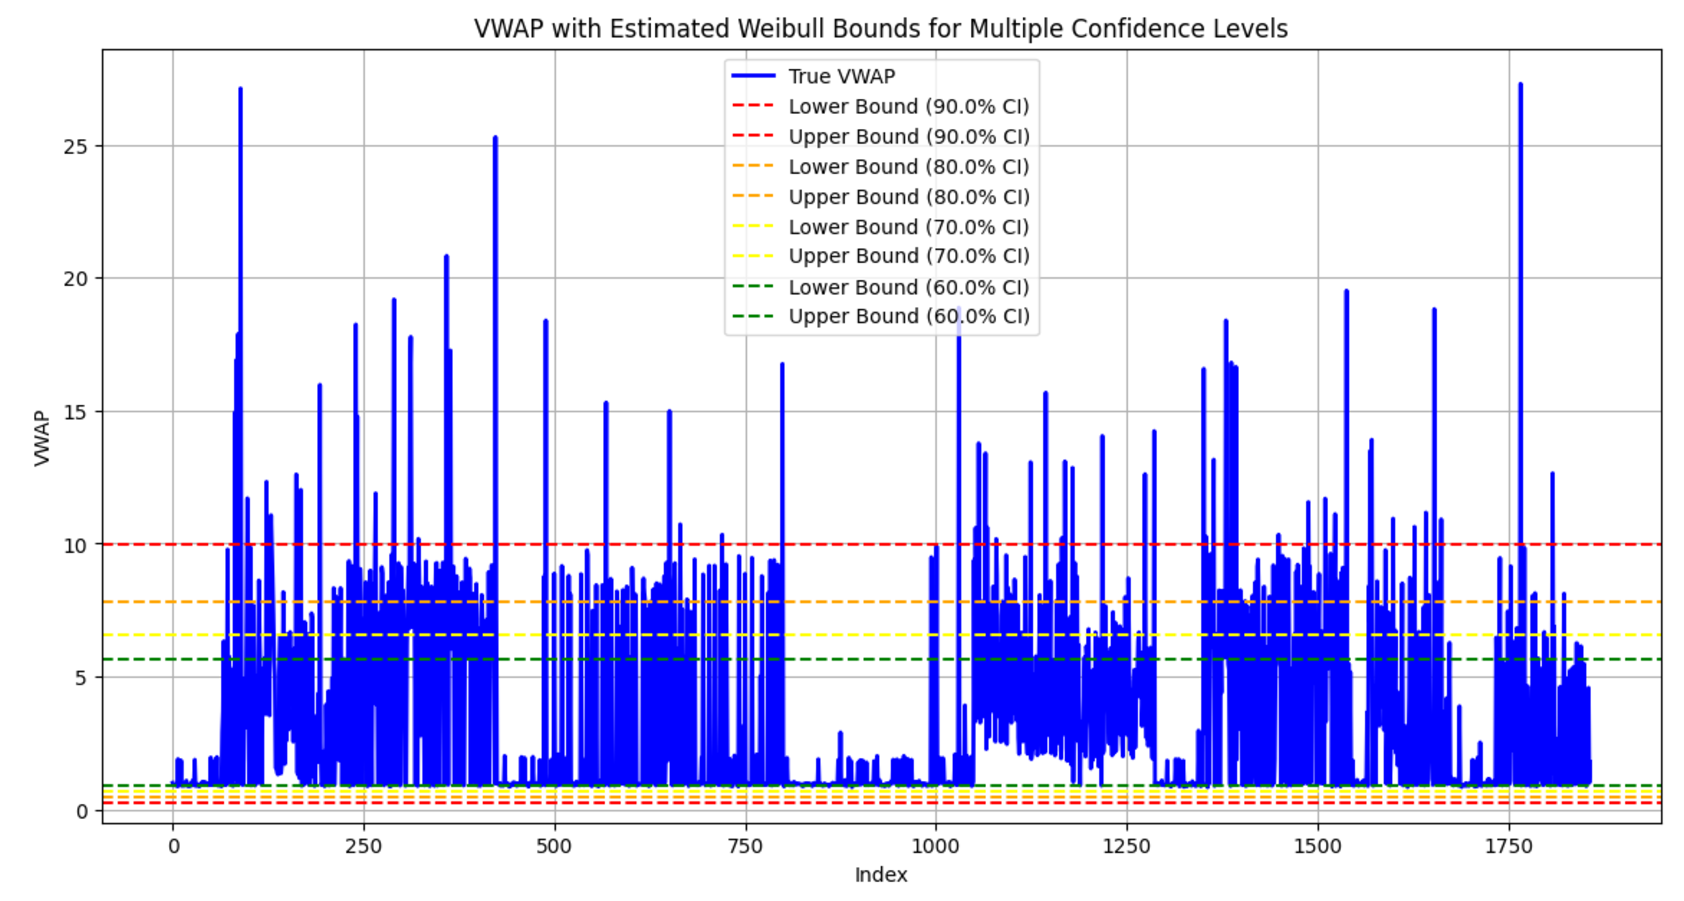
\includegraphics[width=\textwidth]{Chap02/figs/Weibull_Electricity_Consumption.png}
                \caption{Electricity Consumption Dataset.}
            \end{subfigure}

            \begin{subfigure}[b]{0.8\textwidth}
                \centering
                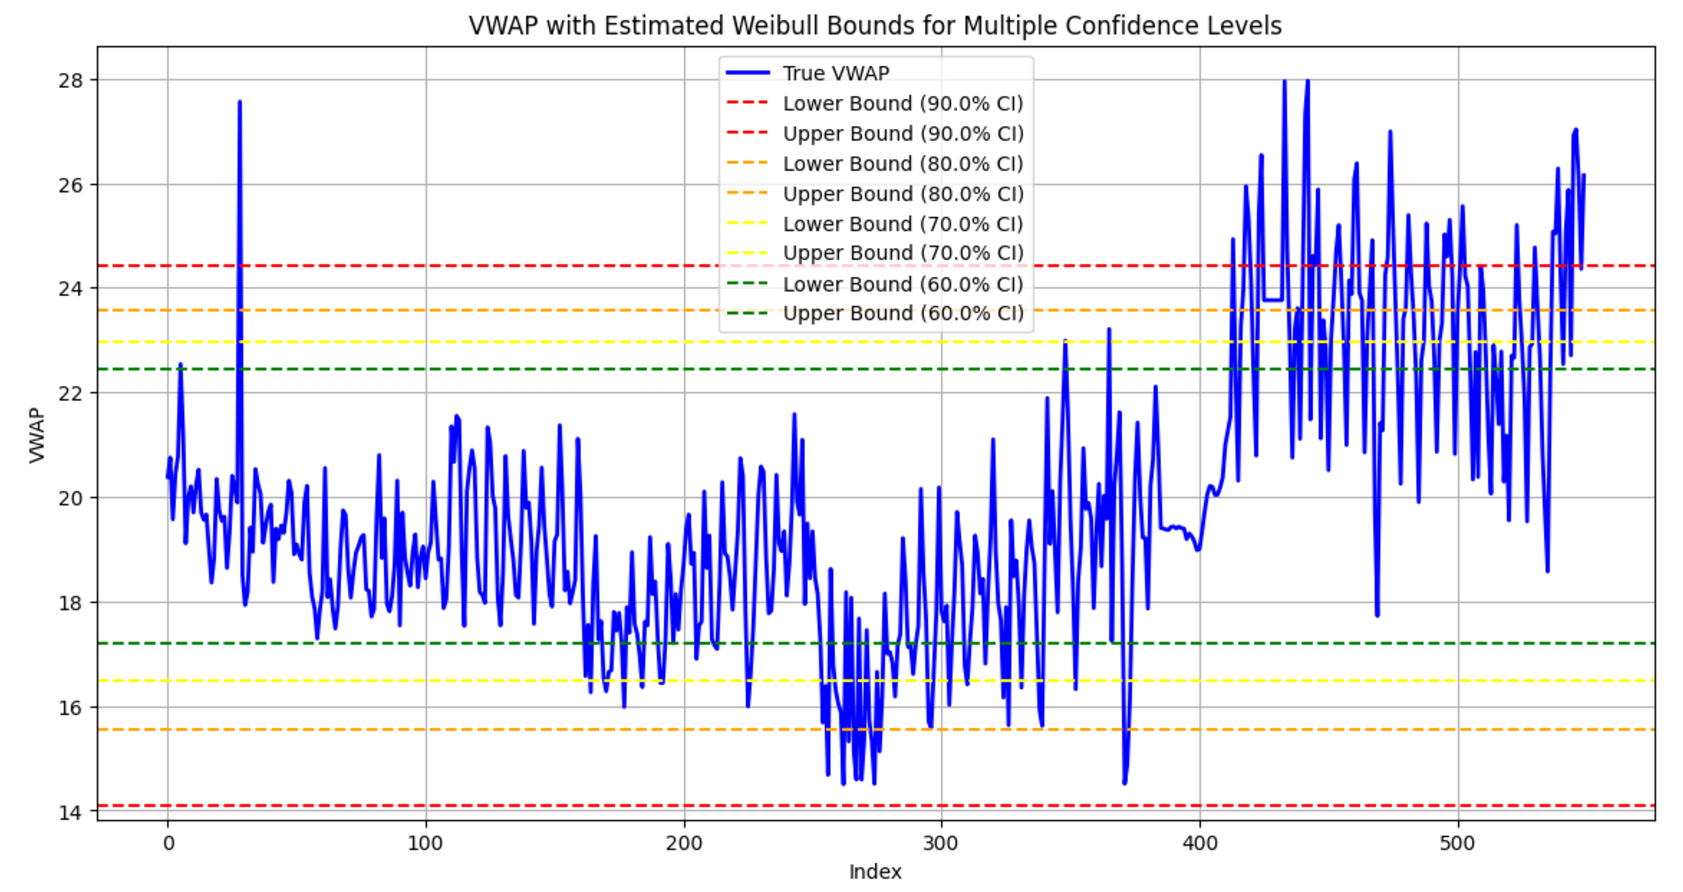
\includegraphics[width=\textwidth]{Chap02/figs/Weibull_Web_Traffic.png}
                \caption{Web Traffic Dataset.}
            \end{subfigure}
        \end{minipage}
    
    \caption{Prediction Intervals for (a) Adani Ports, (b) Asian Paints, (c) Axis Bank, (d) Electricity Consumption Load, (e) Web Traffic datasets obtained using Weibull Distribution method.}
    \label{Fi 3.7}
\end{figure}

\subsection{Discussion}
The results of this study are quite enlightening with respect to the dynamics that characterize probabilistic forecasting as well as the interactions among various methodologies and datasets. Notable in this respect is that non-parametric techniques had a tendency to vary widely in performance between datasets, indicating their effectiveness in modeling uncertainty without requiring strict assumptions about distributions. For instance, the Advanced LUBE method consistently reached an optimal balance between interval coverage and precision, hence it proved to be reliable. Nevertheless, these methods are computationally intensive and may limit their scalability in a real-time application.
In contrast, the parametric approaches presented an interesting duality: they were good at handling structured data, such as electricity consumption, but struggled to capture the complexity of noisy data, such as stock prices and web traffic. This weakness means that these methods are more suitable for domains where the underlying distributions are well defined. The Gaussian distribution was computationally efficient but struggled with coverage accuracy, whereas the Weibull distribution was more versatile across the different datasets.

Interestingly, the model architectures also had a significant role in the forecasting results. CNN and LSTM models performed very well because they are adept at capturing non-linear and temporal dependencies, while GRU and BiLSTM have mixed results, probably because of the complexity of the dataset. These findings bring out the importance of the alignment of model architecture and method selection with the data characteristics.

This research highlights the necessity for hybrid methodologies that combine the accuracy of non-parametric techniques with the effectiveness of parametric frameworks. These strategies have the potential to alleviate the computational limitations associated with non-parametric approaches while preserving adaptability. Furthermore, subsequent investigations might examine adaptive techniques that can fluidly transition between forecasting methods in response to real-time data patterns, thereby facilitating more flexible applications.

Tables \ref{Table 1} to \ref{Table 5} displays the performance of the four non-parametric methods Traditional LUBE, Advanced LUBE, QR-based and Bootstrap-based methods on the five different datasets namely Adani Ports, Asian Paints, Axis Bank, Electricity Consumption and Web Traffic. It displays the results across four evaluation metrics and four different confidence levels (90\%, 80\%, 70\% and 60\%) for each method.

Tables \ref{Table 6} to \ref{Table 10} displays the performance of two parametric methods Gaussian and Weibull Distribution based methods across four different confidence levels and four different evaluation metrics on five different datasets namely Adani Ports, Asian Paints, Axis Bank, Electricity Consumption and Web Traffic.

\newpage
\begin{table*}[!t]
\centering
\caption{Comparative Performance of LUBE, Advanced LUBE, QR-based, Bootstrap Based Methods on Adani Ports dataset.}
\vspace{0.5cm}
\renewcommand{\arraystretch}{0.8} % Adjust the value as needed
\resizebox{\textwidth}{!}{%
\begin{tabular}{|l|l|l|l|l|l|l|}
\hline
\textbf{Method Used} & \textbf{Confidence Level} & \textbf{Model} & \textbf{Avg PICP} & \textbf{Avg PINAW} &  \textbf{Avg ACE} & \textbf{Avg AWE} \\ \hline
\multirow{Traditional LUBE} & 0.6 & BiLSTM & 100 & 31.03 & 40 & 18724.39  \\ \cline{2-7}
& 0.6 & CNN & 100 & 10.07 & 40 & 5661.41 \\ \cline{2-7}
& 0.6 & GRU & 100 & 7.65 & 40 & 4148.68 \\ \cline{2-7}
& 0.6 & LSTM & 100 & 4.94 & 40 & 2460.54 \\ \cline{2-7}
& 0.7 & BiLSTM & 100 & 405.30 & 30 & 252109.41 \\ \cline{2-7}
& 0.7 & CNN & 100 & 9.93 & 30 & 5571.24 \\  \cline{2-7}
& 0.7 & GRU & 100 & 6.63 & 30 & 3513.81 \\ \cline{2-7}
& 0.7 & LSTM & 100 & 4.80 & 30 & 2369.84 \\ \cline{2-7}
& 0.8 & BiLSTM & 100 & 25.62 & 20 & 15358.03 \\ \cline{2-7}
& 0.8 & CNN & 100 & 9.96 & 20 & 5592.60 \\ \cline{2-7}
& 0.8 & GRU & 100 & 7.62 & 20 & 4128.26 \\ \cline{2-7}
& 0.8 & LSTM & 100 & 6.85 & 20 & 3652.41 \\ \cline{2-7}
& 0.9 & BiLSTM & 100 & 624.92 & 10 & 389055.75 \\ \cline{2-7}
& 0.9 & CNN & 100 & 10.01 & 10 & 5619.03 \\ \cline{2-7}
& 0.9 & GRU & 100 & 7.32 & 10 & 3942.56 \\ \cline{2-7}
& 0.9 & LSTM & 100 & 5.10 & 10 & 2557.74 \\ \hline


\multirow{Advanced LUBE} & 0.6 & BiLSTM & 100 & 6.54 & 40 & 3453.78 \\ \cline{2-7}
& 0.6 & CNN & 100 & 3.08 & 40 & 1297.77 \\ \cline{2-7}
& 0.6 & GRU & 100 & 3.21 & 40 & 1376.41 \\ \cline{2-7}
& 0.6 & LSTM & 100 & 6.21 & 40 & 3247.55 \\ \cline{2-7}
& 0.7 & BiLSTM & 100 & 7.18 & 30 & 3854.64 \\ \cline{2-7}
& 0.7 & CNN & 100 & 3.05 & 30 & 1278.93 \\ \cline{2-7}
& 0.7 & GRU & 100 & 3.34 & 30 & 1459.42 \\ \cline{2-7}
& 0.7 & LSTM & 100 & 6.02 & 30 & 3129.68 \\ \cline{2-7}
& 0.8 & BiLSTM & 100 & 6.85 & 20 & 3649.99 \\ \cline{2-7}
& 0.8 & CNN & 100 & 3.14 & 20 & 1333.73 \\ \cline{2-7}
& 0.8 & GRU & 100 & 3.06 & 20 & 1287.54 \\ \cline{2-7}
& 0.8 & LSTM & 100 & 6.90 & 20 & 3676.17 \\ \cline{2-7}
& 0.9 & BiLSTM & 100 & 6.61 & 10 & 3497.79 \\ \cline{2-7}
& 0.9 & CNN & 100 & 3.08 & 10 & 1297.10 \\ \cline{2-7}
& 0.9 & GRU & 100 & 3.47 & 10 & 1537.40 \\ \cline{2-7}
& 0.9 & LSTM & 100 & 6.94 & 10 & 3702.24 \\ \hline


\multirow{QR-based} & 0.6 & BiLSTM & 67.87 & 0.03 & 12.36 & 607.25 \\ \cline{2-7}
& 0.6 & CNN & 79.07 & 0.10 & 21.86 & 562.45 \\ \cline{2-7}
& 0.6 & GRU & 58.87 & 0.02 & 21.24 & 608.68 \\ \cline{2-7}
& 0.6 & LSTM & 70.68 & 0.04 & 26.97 & 600.36 \\ \cline{2-7}
& 0.7 & BiLSTM & 60.72 & 0.03 & 21.29 & 606.88 \\ \cline{2-7}
& 0.7 & CNN & 86.96 & 0.11 & 16.96 & 551.85 \\ \cline{2-7}
& 0.7 & GRU & 72.49 & 0.04 & 21.80 & 601.08 \\ \cline{2-7}
& 0.7 & LSTM & 67.38 & 0.03 & 21.79 & 602.06 \\ \cline{2-7}
& 0.8 & BiLSTM & 86.72 & 0.06 & 8.42 & 587.38 \\ \cline{2-7}
& 0.8 & CNN & 86.74 & 0.13 & 12.12 & 539.85 \\ \cline{2-7}
& 0.8 & GRU & 82.27 & 0.04 & 9.11 & 598.12 \\ \cline{2-7}
& 0.8 & LSTM & 80.08 & 0.06 & 13.03 & 589.16 \\ \cline{2-7}
& 0.9 & BiLSTM & 94.55 & 0.08 & 5.69 & 572.07 \\ \cline{2-7}
& 0.9 & CNN & 95.73 & 0.19 & 5.75 & 507.37 \\ \cline{2-7}
& 0.9 & GRU & 89.80 & 0.07 & 9.49 & 577.76 \\ \cline{2-7}
& 0.9 & LSTM & 97.08 & 0.10 & 7.30 & 561.57 \\ \hline

\multirow{Bootstrap-based} & 0.6 & BiLSTM & 57.48 & 0.17 & 2.55 & 519.87 \\ \cline{2-7}
& 0.6 & CNN & 56.58 & 0.16 & 3.92 & 521.28 \\ \cline{2-7}
& 0.6 & GRU & 58.95 & 0.17 & 2.17 & 519.90 \\ \cline{2-7}
& 0.6 & LSTM & 57.81 & 0.17 & 2.31 & 519.69 \\ \cline{2-7}
& 0.7 & BiLSTM & 67.97 & 0.27 & 2.08 & 453.09 \\ \cline{2-7}
& 0.7 & CNN & 67.34 & 0.28 & 3.03 & 450.21 \\ \cline{2-7}
& 0.7 & GRU & 68.43 & 0.28 & 1.65 & 451.96 \\ \cline{2-7}
& 0.7 & LSTM & 65.88 & 0.27 & 4.17 & 454.46 \\ \cline{2-7}
& 0.8 & BiLSTM & 76.62 & 0.45 & 3.38 & 340.08 \\ \cline{2-7}
& 0.8 & CNN & 77.04 & 0.45 & 3.13 & 341.60 \\ \cline{2-7}
& 0.8 & GRU & 78.29 & 0.46 & 1.71 & 337.02 \\ \cline{2-7}
& 0.8 & LSTM & 78.27 & 0.46 & 1.87 & 338.39 \\ \cline{2-7}
& 0.9 & BiLSTM & 87.53 & 0.68 & 2.47 & 199.80 \\ \cline{2-7}
& 0.9 & CNN & 88.19 & 0.69 & 2.08 & 190.55 \\ \cline{2-7}
& 0.9 & GRU & 88.05 & 0.68 & 1.95 & 198.01 \\ \cline{2-7}
& 0.9 & LSTM & 87.67 & 0.68 & 2.33 & 199.72 \\ \hline
\end{tabular}%
}
\label{Table 1}
\end{table*}

\begin{table*}[!t]
\centering
\caption{Comparative Performance of LUBE, Advanced LUBE, QR-based, Bootstrap Based Methods on Asian Paints dataset.}
\vspace{0.5cm}
\renewcommand{\arraystretch}{0.8} % Adjust the value as needed
\resizebox{\textwidth}{!}{%
\begin{tabular}{|l|l|l|l|l|l|l|}
\hline
\textbf{Method Used} & \textbf{Confidence Level} & \textbf{Model} & \textbf{Avg PICP} & \textbf{Avg PINAW} &  \textbf{Avg ACE} & \textbf{Avg AWE} \\ \hline
\multirow{Traditional LUBE} 
& 0.6 & BiLSTM & 100 & 176.2462 & 40 & 306120.048 \\ \cline{2-7}
& 0.6 & CNN & 100 & 16.7941 & 40 & 27589.0975 \\ \cline{2-7}
& 0.6 & GRU & 100 & 8.7152 & 40 & 13476.9307 \\ \cline{2-7}
& 0.6 & LSTM & 100 & 6.3460 & 40 & 9338.4101 \\ \cline{2-7}
& 0.7 & BiLSTM & 100 & 134.8771 & 30 & 233856.5168 \\ \cline{2-7}
& 0.7 & CNN & 100 & 16.4525 & 30 & 26992.4830 \\ \cline{2-7}
& 0.7 & GRU & 100 & 8.4597 & 30 & 13030.5229 \\ \cline{2-7}
& 0.7 & LSTM & 100 & 6.3955 & 30 & 9424.8555 \\ \cline{2-7}
& 0.8 & BiLSTM & 100 & 107.5393 & 20 & 186102.8086 \\ \cline{2-7}
& 0.8 & CNN & 100 & 16.6753 & 20 & 27381.5852 \\ \cline{2-7}
& 0.8 & GRU & 100 & 8.4415 & 20 & 12998.7874 \\ \cline{2-7}
& 0.8 & LSTM & 100 & 6.4796 & 20 & 9571.7360 \\ \cline{2-7}
& 0.9 & BiLSTM & 100 & 82.2330 & 10 & 141897.7734 \\ \cline{2-7}
& 0.9 & CNN & 100 & 17.2459 & 10 & 28378.3252 \\ \cline{2-7}
& 0.9 & GRU & 100 & 8.8828 & 10 & 13769.6257 \\ \cline{2-7}
& 0.9 & LSTM & 100 & 5.8771 & 10 & 8519.3438 \\ \hline

\multirow{Advanced LUBE} & 0.6 & BiLSTM & 100 & 21.38 & 40 & 35595.10 \\ \cline{2-7}
& 0.6 & CNN & 100 & 4.87 & 40 & 6758.33 \\ \cline{2-7}
& 0.6 & GRU & 100 & 6.44 & 40 & 9493.89 \\ \cline{2-7}
& 0.6 & LSTM & 100 & 11.99 & 40 & 19192.37 \\ \cline{2-7}
& 0.7 & BiLSTM & 100 & 19.89 & 30 & 32988.48 \\ \cline{2-7}
& 0.7 & CNN & 100 & 5.12 & 30 & 7205.28 \\ \cline{2-7}
& 0.7 & GRU & 100 & 6.58 & 30 & 9740.53 \\ \cline{2-7}
& 0.7 & LSTM & 100 & 12.73 & 30 & 20486.20 \\ \cline{2-7}
& 0.8 & BiLSTM & 100 & 18.56 & 20 & 30669.12 \\ \cline{2-7}
& 0.8 & CNN & 100 & 5.04 & 20 & 7062.18 \\ \cline{2-7}
& 0.8 & GRU & 100 & 6.77 & 20 & 10078.24 \\ \cline{2-7}
& 0.8 & LSTM & 100 & 12.21 & 20 & 19584.56 \\ \cline{2-7}
& 0.9 & BiLSTM & 100 & 16.27 & 10 & 26678.04 \\ \cline{2-7}
& 0.9 & CNN & 100 & 5.24 & 10 & 7401.71 \\ \cline{2-7}
& 0.9 & GRU & 100 & 6.20 & 10 & 9086.57 \\ \cline{2-7}
& 0.9 & LSTM & 100 & 13.03 & 10 & 21021.77 \\ \hline

\multirow{QR-based} & 0.6 & BiLSTM & 49.45 & 0.03 & 22.91 & 1702.05 \\ \cline{2-7}
& 0.6 & CNN & 81.00 & 0.13 & 23.66 & 1518.25 \\ \cline{2-7}
& 0.6 & GRU & 35.04 & 0.01 & 33.01 & 1720.67 \\ \cline{2-7}
& 0.6 & LSTM & 39.30 & 0.02 & 35.72 & 1709.96 \\ \cline{2-7}
& 0.7 & BiLSTM & 57.99 & 0.03 & 17.33 & 1689.08 \\ \cline{2-7}
& 0.7 & CNN & 95.28 & 0.20 & 25.28 & 1402.63 \\ \cline{2-7}
& 0.7 & GRU & 52.10 & 0.02 & 26.34 & 1706.18 \\ \cline{2-7}
& 0.7 & LSTM & 74.25 & 0.04 & 18.81 & 1670.70 \\ \cline{2-7}
& 0.8 & BiLSTM & 68.73 & 0.04 & 20.23 & 1670.69 \\ \cline{2-7}
& 0.8 & CNN & 94.19 & 0.21 & 16.91 & 1380.19 \\ \cline{2-7}
& 0.8 & GRU & 81.57 & 0.05 & 9.77 & 1661.94 \\ \cline{2-7}
& 0.8 & LSTM & 79.16 & 0.06 & 19.18 & 1638.10 \\ \cline{2-7}
& 0.9 & BiLSTM & 88.19 & 0.06 & 10.38 & 1637.48 \\ \cline{2-7}
& 0.9 & CNN & 98.68 & 0.32 & 8.68 & 1185.35 \\ \cline{2-7}
& 0.9 & GRU & 84.93 & 0.07 & 9.97 & 1632.32 \\ \cline{2-7}
& 0.9 & LSTM & 71.18 & 0.06 & 23.80 & 1645.33 \\ \hline

\multirow{Bootstrap-based} & 0.6 & BiLSTM & 59.51 & 0.37 & 1.12 & 1102.74 \\ \cline{2-7}
& 0.6 & CNN & 56.96 & 0.37 & 4.45 & 1098.73 \\ \cline{2-7}
& 0.6 & GRU & 58.70 & 0.36 & 1.80 & 1111.23 \\ \cline{2-7}
& 0.6 & LSTM & 57.26 & 0.36 & 3.85 & 1110.84 \\ \cline{2-7}
& 0.7 & BiLSTM & 68.73 & 0.49 & 1.50 & 884.40 \\ \cline{2-7}
& 0.7 & CNN & 67.72 & 0.49 & 3.99 & 892.03 \\ \cline{2-7}
& 0.7 & GRU & 69.01 & 0.49 & 1.35 & 885.19 \\ \cline{2-7}
& 0.7 & LSTM & 69.07 & 0.49 & 1.46 & 885.54 \\ \cline{2-7}
& 0.8 & BiLSTM & 77.19 & 0.63 & 2.81 & 646.05 \\ \cline{2-7}
& 0.8 & CNN & 79.03 & 0.65 & 1.50 & 611.55 \\ \cline{2-7}
& 0.8 & GRU & 78.91 & 0.64 & 1.35 & 627.15 \\ \cline{2-7}
& 0.8 & LSTM & 79.01 & 0.64 & 1.07 & 621.64 \\ \cline{2-7}
& 0.9 & BiLSTM & 89.08 & 0.79 & 1.28 & 369.51 \\ \cline{2-7}
& 0.9 & CNN & 88.31 & 0.78 & 2.19 & 383.92 \\ \cline{2-7}
& 0.9 & GRU & 88.70 & 0.79 & 1.30 & 373.43 \\ \cline{2-7}
& 0.9 & LSTM & 89.48 & 0.79 & 0.97 & 369.39 \\ \hline
\end{tabular}%
}
\label{Table 2}
\end{table*}

\begin{table*}[!t]
\centering
\caption{Comparative Performance of LUBE, Advanced LUBE, QR-based, Bootstrap Based Methods on Axis Bank dataset.}
\vspace{0.5cm}
\renewcommand{\arraystretch}{0.8} % Adjust the value as needed
\resizebox{\textwidth}{!}{%
\begin{tabular}{|l|l|l|l|l|l|l|}
\hline
\textbf{Method Used} & \textbf{Confidence Level} & \textbf{Model} & \textbf{Avg PICP} & \textbf{Avg PINAW} &  \textbf{Avg ACE} & \textbf{Avg AWE} \\ \hline
\multirow{Traditional LUBE} & 0.6 & BiLSTM & 100 & 142.23 & 40 & 71594.44 \\ \cline{2-7}
& 0.6 & CNN & 100 & 21.70 & 40 & 10492.69 \\ \cline{2-7}
& 0.6 & GRU & 100 & 13.41 & 40 & 6290.57 \\ \cline{2-7}
& 0.6 & LSTM & 100 & 10.36 & 40 & 4746.86 \\ \cline{2-7}
& 0.7 & BiLSTM & 100 & 84.23 & 30 & 42192.68 \\ \cline{2-7}
& 0.7 & CNN & 100 & 21.98 & 30 & 10635.94 \\ \cline{2-7}
& 0.7 & GRU & 100 & 14.67 & 30 & 6932.03 \\ \cline{2-7}
& 0.7 & LSTM & 100 & 8.15 & 30 & 3623.44 \\ \cline{2-7}
& 0.8 & BiLSTM & 100 & 30683.37 & 20 & 15554427.52 \\ \cline{2-7}
& 0.8 & CNN & 100 & 22.58 & 20 & 10939.10 \\ \cline{2-7}
& 0.8 & GRU & 100 & 15.97 & 20 & 7587.76 \\ \cline{2-7}
& 0.8 & LSTM & 100 & 9.98 & 20 & 4553.34 \\ \cline{2-7}
& 0.9 & BiLSTM & 100 & 110.06 & 10 & 55289.93 \\ \cline{2-7}
& 0.9 & CNN & 100 & 22.11 & 10 & 10700.12 \\ \cline{2-7}
& 0.9 & GRU & 100 & 16.70 & 10 & 7957.61 \\ \cline{2-7}
& 0.9 & LSTM & 100 & 10.35 & 10 & 4741.71 \\ \hline

\multirow{Advanced LUBE} & 0.6 & BiLSTM & 100 & 19.02 & 40 & 9136.65 \\ \cline{2-7}
& 0.6 & CNN & 100 & 6.97 & 40 & 3027.38 \\ \cline{2-7}
& 0.6 & GRU & 100 & 7.53 & 40 & 3311.35 \\ \cline{2-7}
& 0.6 & LSTM & 100 & 15.30 & 40 & 7248.18 \\ \cline{2-7}
& 0.7 & BiLSTM & 100 & 17.66 & 30 & 8445.44 \\ \cline{2-7}
& 0.7 & CNN & 100 & 7.11 & 30 & 3098.77 \\ \cline{2-7}
& 0.7 & GRU & 100 & 7.49 & 30 & 3287.88 \\ \cline{2-7}
& 0.7 & LSTM & 100 & 14.99 & 30 & 7091.83 \\ \cline{2-7}
& 0.8 & BiLSTM & 100 & 19.64 & 20 & 9449.07 \\ \cline{2-7}
& 0.8 & CNN & 100 & 6.86 & 20 & 2972.82 \\ \cline{2-7}
& 0.8 & GRU & 100 & 7.77 & 20 & 3432.81 \\ \cline{2-7}
& 0.8 & LSTM & 100 & 15.69 & 20 & 7448.36 \\ \cline{2-7}
& 0.9 & BiLSTM & 100 & 21.82 & 10 & 10554.26 \\ \cline{2-7}
& 0.9 & CNN & 100 & 6.64 & 10 & 2861.38 \\ \cline{2-7}
& 0.9 & GRU & 100 & 7.10 & 10 & 3094.89 \\ \cline{2-7}
& 0.9 & LSTM & 100 & 16.27 & 10 & 7743.09 \\ \hline

\multirow{QR-based} & 0.6 & BiLSTM & 63.97 & 0.05 & 16.28 & 481.88 \\ \cline{2-7}
& 0.6 & CNN & 78.04 & 0.17 & 25.41 & 423.17 \\ \cline{2-7}
& 0.6 & GRU & 74.13 & 0.06 & 16.84 & 476.30 \\ \cline{2-7}
& 0.6 & LSTM & 81.17 & 0.09 & 24.06 & 460.57 \\ \cline{2-7}
& 0.7 & BiLSTM & 82.44 & 0.08 & 18.72 & 466.64 \\ \cline{2-7}
& 0.7 & CNN & 93.64 & 0.24 & 23.64 & 384.16 \\ \cline{2-7}
& 0.7 & GRU & 78.98 & 0.07 & 11.27 & 472.55 \\ \cline{2-7}
& 0.7 & LSTM & 87.99 & 0.11 & 20.52 & 453.45 \\ \cline{2-7}
& 0.8 & BiLSTM & 86.69 & 0.09 & 8.15 & 459.56 \\ \cline{2-7}
& 0.8 & CNN & 96.35 & 0.30 & 16.35 & 355.55 \\ \cline{2-7}
& 0.8 & GRU & 88.24 & 0.09 & 8.89 & 462.92 \\ \cline{2-7}
& 0.8 & LSTM & 84.69 & 0.09 & 14.30 & 461.12 \\ \cline{2-7}
& 0.9 & BiLSTM & 96.65 & 0.15 & 6.74 & 429.74 \\ \cline{2-7}
& 0.9 & CNN & 98.25 & 0.41 & 8.25 & 299.18 \\ \cline{2-7}
& 0.9 & GRU & 95.96 & 0.17 & 7.53 & 423.20 \\ \cline{2-7}
& 0.9 & LSTM & 89.23 & 0.13 & 9.45 & 442.80 \\ \hline

\multirow{Bootstrap-based} & 0.6 & BiLSTM & 59.80 & 0.47 & 2.19 & 268.87 \\ \cline{2-7}
& 0.6 & CNN & 61.04 & 0.47 & 2.96 & 267.34 \\ \cline{2-7}
& 0.6 & GRU & 60.68 & 0.47 & 1.79 & 269.28 \\ \cline{2-7}
& 0.6 & LSTM & 59.50 & 0.47 & 2.31 & 269.05 \\ \cline{2-7}
& 0.7 & BiLSTM & 70.53 & 0.56 & 1.91 & 224.65 \\ \cline{2-7}
& 0.7 & CNN & 71.46 & 0.56 & 2.96 & 220.82 \\ \cline{2-7}
& 0.7 & GRU & 72.65 & 0.56 & 2.97 & 224.17 \\ \cline{2-7}
& 0.7 & LSTM & 68.44 & 0.55 & 2.84 & 226.77 \\ \cline{2-7}
& 0.8 & BiLSTM & 79.60 & 0.63 & 1.36 & 188.36 \\ \cline{2-7}
& 0.8 & CNN & 73.03 & 0.62 & 7.17 & 191.75 \\ \cline{2-7}
& 0.8 & GRU & 80.23 & 0.63 & 0.91 & 186.70 \\ \cline{2-7}
& 0.8 & LSTM & 79.46 & 0.63 & 1.17 & 186.19 \\ \cline{2-7}
& 0.9 & BiLSTM & 88.88 & 0.72 & 1.12 & 142.82 \\ \cline{2-7}
& 0.9 & CNN & 87.50 & 0.72 & 2.50 & 140.65 \\ \cline{2-7}
& 0.9 & GRU & 88.87 & 0.72 & 1.13 & 142.78 \\ \cline{2-7}
& 0.9 & LSTM & 85.02 & 0.71 & 4.98 & 148.03 \\ \hline

\end{tabular}%
}
\label{Table 3}
\end{table*}

\begin{table*}[!t]
\centering
\caption{Comparative Performance of LUBE, Advanced LUBE, QR-based, Bootstrap Based Methods on Electricity Consumption dataset.}
\vspace{0.5cm}
\renewcommand{\arraystretch}{0.8} % Adjust the value as needed
\resizebox{\textwidth}{!}{%
\begin{tabular}{|l|l|l|l|l|l|l|}
\hline
\textbf{Method Used} & \textbf{Confidence Level} & \textbf{Model} & \textbf{Avg PICP} & \textbf{Avg PINAW} &  \textbf{Avg ACE} & \textbf{Avg AWE} \\ \hline

\multirow{Traditional LUBE} & 0.6 & BiLSTM & 100.00 & 3.69 & 40 & 71.06 \\ \cline{2-7}
& 0.6 & CNN & 100.00 & 4.15 & 40 & 83.35 \\ \cline{2-7}
& 0.6 & GRU & 100.00 & 2.44 & 40 & 38.01 \\ \cline{2-7}
& 0.6 & LSTM & 100.00 & 2.24 & 40 & 32.70 \\ \cline{2-7}
& 0.7 & BiLSTM & 100.00 & 3.80 & 30 & 74.14 \\ \cline{2-7}
& 0.7 & CNN & 100.00 & 4.00 & 30 & 79.19 \\ \cline{2-7}
& 0.7 & GRU & 100.00 & 1.70 & 30 & 18.59 \\ \cline{2-7}
& 0.7 & LSTM & 100.00 & 2.68 & 30 & 44.36 \\ \cline{2-7}
& 0.8 & BiLSTM & 100.00 & 5.71 & 20 & 124.41 \\ \cline{2-7}
& 0.8 & CNN & 100.00 & 4.10 & 20 & 82.06 \\ \cline{2-7}
& 0.8 & GRU & 100.00 & 2.81 & 20 & 47.74 \\ \cline{2-7}
& 0.8 & LSTM & 100.00 & 2.75 & 20 & 46.31 \\ \cline{2-7}
& 0.9 & BiLSTM & 100.00 & 4.16 & 10 & 83.67 \\ \cline{2-7}
& 0.9 & CNN & 100.00 & 4.19 & 10 & 84.42 \\ \cline{2-7}
& 0.9 & GRU & 100.00 & 2.25 & 10 & 33.16 \\ \cline{2-7}
& 0.9 & LSTM & 100.00 & 1.97 & 10 & 25.68 \\ \hline



\multirow{Advanced LUBE} 
& 0.6 & BiLSTM & 100.00 & 2.02 & 40 & 27.09 \\ \cline{2-7}
& 0.6 & CNN & 99.68 & 0.99 & 39.68 & 0.90 \\ \cline{2-7}
& 0.6 & GRU & 100.00 & 1.39 & 40 & 10.31 \\ \cline{2-7}
& 0.6 & LSTM & 100.00 & 2.07 & 40 & 28.23 \\ \cline{2-7}
& 0.7 & BiLSTM & 100.00 & 1.82 & 30 & 21.70 \\ \cline{2-7}
& 0.7 & CNN & 99.67 & 0.99 & 29.67 & 0.65 \\ \cline{2-7}
& 0.7 & GRU & 100.00 & 1.48 & 30 & 12.79 \\ \cline{2-7}
& 0.7 & LSTM & 100.00 & 1.98 & 30 & 25.95 \\ \cline{2-7}
& 0.8 & BiLSTM & 100.00 & 1.99 & 20 & 26.15 \\ \cline{2-7}
& 0.8 & CNN & 99.67 & 0.98 & 19.67 & 1.08 \\ \cline{2-7}
& 0.8 & GRU & 100.00 & 1.36 & 20 & 9.52 \\ \cline{2-7}
& 0.8 & LSTM & 100.00 & 2.32 & 20 & 35.01 \\ \cline{2-7}
& 0.9 & BiLSTM & 100.00 & 1.66 & 10 & 17.32 \\ \cline{2-7}
& 0.9 & CNN & 99.69 & 1.01 & 9.69 & 0.92 \\ \cline{2-7}
& 0.9 & GRU & 100.00 & 1.35 & 10 & 9.32 \\ \cline{2-7}
& 0.9 & LSTM & 100.00 & 2.21 & 10 & 32.04 \\ \hline


\multirow{QR-based} 
& 0.6 & BiLSTM & 46.69 & 0.1443 & 13.31 & 22.63 \\ \cline{2-7}
& 0.6 & CNN & 56.94 & 0.1667 & 10.44 & 22.03 \\ \cline{2-7}
& 0.6 & GRU & 50.04 & 0.1494 & 10.70 & 22.49 \\ \cline{2-7}
& 0.6 & LSTM & 65.47 & 0.1605 & 12.68 & 22.20 \\ \cline{2-7}
& 0.7 & BiLSTM & 70.76 & 0.1980 & 4.37 & 21.21 \\ \cline{2-7}
& 0.7 & CNN & 73.78 & 0.2004 & 4.11 & 21.14 \\ \cline{2-7}
& 0.7 & GRU & 65.61 & 0.1838 & 10.45 & 21.58 \\ \cline{2-7}
& 0.7 & LSTM & 74.86 & 0.1997 & 12.18 & 21.16 \\ \cline{2-7}
& 0.8 & BiLSTM & 78.92 & 0.2372 & 6.69 & 20.17 \\ \cline{2-7}
& 0.8 & CNN & 82.73 & 0.2484 & 5.94 & 19.87 \\ \cline{2-7}
& 0.8 & GRU & 81.98 & 0.2278 & 5.22 & 20.42 \\ \cline{2-7}
& 0.8 & LSTM & 81.51 & 0.2473 & 10.86 & 19.90 \\ \cline{2-7}
& 0.9 & BiLSTM & 88.35 & 0.2900 & 4.82 & 18.77 \\ \cline{2-7}
& 0.9 & CNN & 87.52 & 0.3027 & 5.66 & 18.44 \\ \cline{2-7}
& 0.9 & GRU & 90.65 & 0.3133 & 3.58 & 18.16 \\ \cline{2-7}
& 0.9 & LSTM & 83.96 & 0.3342 & 15.01 & 17.60 \\ \hline


\multirow{Bootstrap-based} 
& 0.6 & BiLSTM & 24.42 & 0.0846 & 35.58 & 24.20 \\ \cline{2-7}
& 0.6 & CNN & 24.42 & 0.0734 & 35.58 & 24.50 \\ \cline{2-7}
& 0.6 & GRU & 19.50 & 0.0777 & 40.50 & 24.39 \\ \cline{2-7}
& 0.6 & LSTM & 21.01 & 0.0762 & 38.99 & 24.43 \\ \cline{2-7}
& 0.7 & BiLSTM & 28.06 & 0.1064 & 41.94 & 23.63 \\ \cline{2-7}
& 0.7 & CNN & 32.23 & 0.0930 & 37.77 & 23.98 \\ \cline{2-7}
& 0.7 & GRU & 28.20 & 0.1040 & 41.80 & 23.69 \\ \cline{2-7}
& 0.7 & LSTM & 33.92 & 0.1029 & 36.08 & 23.72 \\ \cline{2-7}
& 0.8 & BiLSTM & 34.60 & 0.1198 & 45.40 & 23.27 \\ \cline{2-7}
& 0.8 & CNN & 32.70 & 0.1157 & 47.30 & 23.38 \\ \cline{2-7}
& 0.8 & GRU & 31.76 & 0.1152 & 48.24 & 23.39 \\ \cline{2-7}
& 0.8 & LSTM & 37.70 & 0.1184 & 42.30 & 23.31 \\ \cline{2-7}
& 0.9 & BiLSTM & 45.04 & 0.1376 & 44.96 & 22.80 \\ \cline{2-7}
& 0.9 & CNN & 43.88 & 0.1316 & 46.12 & 22.96 \\ \cline{2-7}
& 0.9 & GRU & 41.40 & 0.1335 & 48.60 & 22.91 \\ \cline{2-7}
& 0.9 & LSTM & 52.59 & 0.1297 & 37.41 & 23.01 \\ \hline

\end{tabular}%
}
\label{Table 4}
\end{table*}


\begin{table*}[!t]
\centering
\caption{Comparative Performance of LUBE, Advanced LUBE, QR-based, Bootstrap Based Methods on Web Traffic dataset.}
\vspace{0.5cm}
\renewcommand{\arraystretch}{0.8} % Adjust the value as needed
\resizebox{\textwidth}{!}{%
\begin{tabular}{|l|l|l|l|l|l|l|}
\hline
\textbf{Method Used} & \textbf{Confidence Level} & \textbf{Model} & \textbf{Avg PICP} & \textbf{Avg PINAW} &  \textbf{Avg ACE} & \textbf{Avg AWE} \\ \hline

\multirow{Traditional LUBE} 
& 0.6 & BiLSTM & 100 & 10.5871 & 40 & 89.2555 \\ \cline{2-7}
& 0.6 & CNN & 100 & 5.3765 & 40 & 40.7450 \\ \cline{2-7}
& 0.6 & GRU & 100 & 3.9920 & 40 & 27.8559 \\ \cline{2-7}
& 0.6 & LSTM & 100 & 3.7757 & 40 & 25.8415 \\ \cline{2-7}
& 0.7 & BiLSTM & 100 & 10.0964 & 30 & 84.6871 \\ \cline{2-7}
& 0.7 & CNN & 100 & 5.2022 & 30 & 39.1221 \\ \cline{2-7}
& 0.7 & GRU & 100 & 4.0640 & 30 & 28.5260 \\ \cline{2-7}
& 0.7 & LSTM & 100 & 2.8798 & 30 & 17.5013 \\ \cline{2-7}
& 0.8 & BiLSTM & 100 & 10.1790 & 20 & 85.4565 \\ \cline{2-7}
& 0.8 & CNN & 100 & 5.2952 & 20 & 39.9882 \\ \cline{2-7}
& 0.8 & GRU & 100 & 4.1002 & 20 & 28.8626 \\ \cline{2-7}
& 0.8 & LSTM & 100 & 4.0289 & 20 & 28.1994 \\ \cline{2-7}
& 0.9 & BiLSTM & 100 & 10.4536 & 10 & 88.0132 \\ \cline{2-7}
& 0.9 & CNN & 100 & 5.2567 & 10 & 39.6294 \\ \cline{2-7}
& 0.9 & GRU & 100 & 4.0724 & 10 & 28.6041 \\ \cline{2-7}
& 0.9 & LSTM & 100 & 3.7530 & 10 & 25.6306 \\ \hline

\multirow{Advanced LUBE} 
& 0.6 & BiLSTM & 100 & 5.1715 & 40 & 38.8365 \\ \cline{2-7}
& 0.6 & CNN & 99.9628 & 1.8441 & 39.9628 & 7.8588 \\ \cline{2-7}
& 0.6 & GRU & 100 & 2.9044 & 40 & 17.7303 \\ \cline{2-7}
& 0.6 & LSTM & 100 & 4.5065 & 40 & 32.6452 \\ \cline{2-7}
& 0.7 & BiLSTM & 100 & 4.6309 & 30 & 33.8035 \\ \cline{2-7}
& 0.7 & CNN & 98.9218 & 1.7859 & 28.9218 & 7.3169 \\ \cline{2-7}
& 0.7 & GRU & 100 & 3.1460 & 30 & 19.9797 \\ \cline{2-7}
& 0.7 & LSTM & 100 & 4.1576 & 30 & 29.3974 \\ \cline{2-7}
& 0.8 & BiLSTM & 100 & 5.0116 & 20 & 37.3477 \\ \cline{2-7}
& 0.8 & CNN & 99.4170 & 1.7916 & 19.4170 & 7.3702 \\ \cline{2-7}
& 0.8 & GRU & 100 & 3.0457 & 20 & 19.0454 \\ \cline{2-7}
& 0.8 & LSTM & 100 & 4.0881 & 20 & 28.7499 \\ \cline{2-7}
& 0.9 & BiLSTM & 100 & 4.9196 & 10 & 36.4912 \\ \cline{2-7}
& 0.9 & CNN & 99.1939 & 1.6862 & 9.1939 & 6.3889 \\ \cline{2-7}
& 0.9 & GRU & 100 & 3.1565 & 10 & 20.0771 \\ \cline{2-7}
& 0.9 & LSTM & 100 & 4.2867 & 10 & 30.5994 \\ \hline

\multirow{QR-based} 
& 0.6 & BiLSTM & 21.4634 & 0.2639 & 38.5366 & 6.8529 \\ \cline{2-7}
& 0.6 & CNN & 15.1220 & 0.2586 & 44.8780 & 6.9025 \\ \cline{2-7}
& 0.6 & GRU & 33.7805 & 0.3303 & 26.2195 & 6.2347 \\ \cline{2-7}
& 0.6 & LSTM & 19.6341 & 0.2617 & 40.3659 & 6.8733 \\ \cline{2-7}
& 0.7 & BiLSTM & 25.8537 & 0.3031 & 44.1463 & 6.4879 \\ \cline{2-7}
& 0.7 & CNN & 18.4146 & 0.3330 & 51.5854 & 6.2101 \\ \cline{2-7}
& 0.7 & GRU & 43.2927 & 0.3703 & 26.7073 & 5.8625 \\ \cline{2-7}
& 0.7 & LSTM & 25.2439 & 0.2937 & 44.7561 & 6.5756 \\ \cline{2-7}
& 0.8 & BiLSTM & 50.2439 & 0.4557 & 29.7561 & 5.0670 \\ \cline{2-7}
& 0.8 & CNN & 24.3902 & 0.4074 & 55.6098 & 5.5174 \\ \cline{2-7}
& 0.8 & GRU & 52.9268 & 0.4617 & 27.0732 & 5.0117 \\ \cline{2-7}
& 0.8 & LSTM & 40.6098 & 0.4011 & 39.3902 & 5.5761 \\ \cline{2-7}
& 0.9 & BiLSTM & 58.7805 & 0.5750 & 31.2195 & 3.9564 \\ \cline{2-7}
& 0.9 & CNN & 19.5122 & 0.4978 & 70.4878 & 4.6753 \\ \cline{2-7}
& 0.9 & GRU & 50.3659 & 0.4454 & 39.6341 & 5.1632 \\ \cline{2-7}
& 0.9 & LSTM & 45.0000 & 0.4244 & 45.0000 & 5.3588 \\ \hline

\multirow{Bootstrap-based} 
& 0.6 & BiLSTM & 19.5122 & 0.2041 & 40.4878 & 7.4098 \\ \cline{2-7}
& 0.6 & CNN & 28.1707 & 0.2416 & 31.8293 & 7.0603 \\ \cline{2-7}
& 0.6 & GRU & 20.1220 & 0.2004 & 39.8780 & 7.4442 \\ \cline{2-7}
& 0.6 & LSTM & 19.1463 & 0.2147 & 40.8537 & 7.3116 \\ \cline{2-7}
& 0.7 & BiLSTM & 20.3659 & 0.2337 & 49.6341 & 7.1339 \\ \cline{2-7}
& 0.7 & CNN & 35.3659 & 0.2972 & 34.6341 & 6.5429 \\ \cline{2-7}
& 0.7 & GRU & 26.8293 & 0.2754 & 43.1707 & 6.7694 \\ \cline{2-7}
& 0.7 & LSTM & 21.8049 & 0.2436 & 48.1951 & 7.0651 \\ \cline{2-7}
& 0.8 & BiLSTM & 38.7073 & 0.3137 & 41.2927 & 5.8068 \\ \cline{2-7}
& 0.8 & CNN & 43.1707 & 0.3291 & 26.8293 & 5.9821 \\ \cline{2-7}
& 0.8 & GRU & 33.7805 & 0.3092 & 36.2195 & 5.9619 \\ \cline{2-7}
& 0.8 & LSTM & 24.3902 & 0.2824 & 45.6098 & 6.1043 \\ \cline{2-7}
& 0.9 & BiLSTM & 45.3659 & 0.4005 & 34.6341 & 4.4732 \\ \cline{2-7}
& 0.9 & CNN & 51.7073 & 0.3894 & 18.2927 & 4.4840 \\ \cline{2-7}
& 0.9 & GRU & 45.2195 & 0.3735 & 34.7805 & 4.5675 \\ \cline{2-7}
& 0.9 & LSTM & 46.4634 & 0.3952 & 33.5366 & 4.5153 \\ \hline


\end{tabular}%
}
\label{Table 5}
\end{table*}


\begin{table*}[!t]
%\centering
\caption{Comparative Performance of Gaussian Distribution and Weibull Distribution based Methods on Adani Ports dataset.}
\vspace{0.5cm}
\renewcommand{\arraystretch}{1} % Adjust the value as needed
\resizebox{\textwidth}{!}{%
\begin{tabular}{|l|l|l|l|l|l|}
\hline
\textbf{Method Used} & \textbf{Confidence Level} & \textbf{Avg PICP} & \textbf{Avg PINAW} &  \textbf{Avg ACE} & \textbf{Avg AWE} \\ \hline
\multirow{Gaussian Distribution} & 0.6 & 55.75 & 0.09 & 4.25 & 163.11 \\ \cline{2-6}
& 0.7 & 71.19 & 0.12 & 1.19 & 200.87 \\ \cline{2-6}
& 0.8 & 88.32 & 0.14 & 8.32 & 248.38 \\ \cline{2-6}
& 0.9 & 91.36 & 0.19 & 1.36 & 318.79 \\ \hline

\multirow{Weibull Distribution} & 0.6 & 56.08 & 0.27 & 3.92 & 323.55 \\ \cline{2-6}
& 0.7 & 65.77 & 0.33 & 4.23 & 395.97 \\ \cline{2-6}
& 0.8 & 86.66 & 0.40 & 6.66 & 485.05 \\ \cline{2-6}
& 0.9 & 92.50 & 0.51 & 2.50 & 612.33 \\ \hline

\end{tabular}%
}
\label{Table 6}
\end{table*}

\begin{table*}[!t]
%\centering
\caption{Comparative Performance of Gaussian Distribution and Weibull Distribution based Methods on Asian Paints dataset.}
\vspace{0.5cm}
\renewcommand{\arraystretch}{1} % Adjust the value as needed
\resizebox{\textwidth}{!}{%
\begin{tabular}{|l|l|l|l|l|l|}
\hline
\textbf{Method Used} & \textbf{Confidence Level} & \textbf{Avg PICP} & \textbf{Avg PINAW} &  \textbf{Avg ACE} & \textbf{Avg AWE} \\ \hline
\multirow{Gaussian Distribution} & 0.6 & 63.38 & 0.34 & 3.38 & 904.70 \\ \cline{2-6}
& 0.7 & 83.58 & 0.42 & 13.58 & 1114.12 \\ \cline{2-6}
& 0.8 & 86.78 & 0.52 & 6.78 & 1377.61 \\ \cline{2-6}
& 0.9 & 90.93 & 0.66 & 0.93 & 1768.14 \\ \hline

\multirow{Weibull Distribution} & 0.6 & 56.26 & 0.31 & 3.74 & 1558.04 \\ \cline{2-6}
& 0.7 & 68.69 & 0.38 & 1.31 & 1923.42 \\ \cline{2-6}
& 0.8 & 86.28 & 0.48 & 6.28 & 2388.31 \\ \cline{2-6}
& 0.9 & 93.35 & 0.62 & 3.35 & 3092.62 \\ \hline

\end{tabular}%
}
\label{Table 7}
\end{table*}

\begin{table*}[!t]
%\centering
\caption{Comparative Performance of Gaussian Distribution and Weibull Distribution based Methods on Axis Bank dataset.}
\vspace{0.5cm}
\renewcommand{\arraystretch}{1} % Adjust the value as needed
\resizebox{\textwidth}{!}{%
\begin{tabular}{|l|l|l|l|l|l|}
\hline
\textbf{Method Used} & \textbf{Confidence Level} & \textbf{Avg PICP} & \textbf{Avg PINAW} &  \textbf{Avg ACE} & \textbf{Avg AWE} \\ \hline
\multirow{Gaussian Distribution} & 0.6 & 53.13 & 0.14 & 6.87 & 367.43 \\ \cline{2-6}
& 0.7 & 60.25 & 0.17 & 9.75 & 452.47 \\ \cline{2-6}
& 0.8 & 84.41 & 0.21 & 4.41 & 559.48 \\ \cline{2-6}
& 0.9 & 92.82 & 0.27 & 2.82 & 718.10 \\ \hline

\multirow{Weibull Distribution} & 0.6 & 52.90 & 0.37 & 7.10 & 749.62 \\ \cline{2-6}
& 0.7 & 61.23 & 0.46 & 8.77 & 928.27 \\ \cline{2-6}
& 0.8 & 71.70 & 0.58 &  8.30 & 1157.98 \\ \cline{2-6}
& 0.9 & 82.72 & 0.76 & 7.28 & 1511.76 \\ \hline
\end{tabular}%
}
\label{Table 8}
\end{table*}

\begin{table*}[!t]
%\centering
\caption{Comparative Performance of Gaussian Distribution and Weibull Distribution based Methods on Electricity Consumption dataset.}
\vspace{0.5cm}
\renewcommand{\arraystretch}{1} % Adjust the value as needed
\resizebox{\textwidth}{!}{%
\begin{tabular}{|l|l|l|l|l|l|}
\hline
\textbf{Method Used} & \textbf{Confidence Level} & \textbf{Avg PICP} & \textbf{Avg PINAW} &  \textbf{Avg ACE} & \textbf{Avg AWE} \\ \hline
\multirow{Gaussian Distribution} & 0.6 & 79.60 & 0.003 & 19.60 & 2.94 \\ \cline{2-6}
& 0.7 & 83.36 & 0.004 & 13.36 & 3.62 \\ \cline{2-6}
& 0.8 & 87.41 & 0.005 & 7.41 & 4.48 \\ \cline{2-6}
& 0.9 & 94.30 & 0.006 & 4.30 & 5.74 \\ \hline

\multirow{Weibull Distribution} & 0.6 & 64.10 & 0.18 & 4.10 &  4.71\\ \cline{2-6}
& 0.7 & 80.30 & 0.22 & 10.30 & 5.86 \\ \cline{2-6}
& 0.8 & 86.54 & 0.27 & 6.54 & 7.36 \\ \cline{2-6}
& 0.9 & 96.77 & 0.37 & 6.77 & 9.73 \\ \hline

\end{tabular}%
}
\label{Table 9}
\end{table*}
%\clearpage

\begin{table*}[!t] % Force the table to the top of the page
\centering
\caption{Comparative Performance of Gaussian Distribution and Weibull Distribution based Methods on Web Traffic dataset.}
\vspace{0.5cm}
\renewcommand{\arraystretch}{1} % Adjust the value as needed
\resizebox{\textwidth}{!}{%
\begin{tabular}{|l|l|l|l|l|l|}
\hline
\textbf{Method Used} & \textbf{Confidence Level} & \textbf{Avg PICP} & \textbf{Avg PINAW} &  \textbf{Avg ACE} & \textbf{Avg AWE} \\ \hline
\multirow{Gaussian Distribution} & 0.6 & 62.54 & 0.008 & 2.54 & 2.21 \\ \cline{2-6}
& 0.7 & 71.27 & 0.009 & 1.27 & 2.72 \\ \cline{2-6}
& 0.8 & 78.73 & 0.01 & 1.27 & 3.37 \\ \cline{2-6}
& 0.9 & 89.45 & 0.15 & 0.55 & 4.32 \\ \hline

\multirow{Weibull Distribution} & 0.6 & 70 & 0.39 & 10 & 5.25 \\ \cline{2-6}
& 0.7 & 77.45 & 0.48 & 7.45 & 6.48 \\ \cline{2-6}
& 0.8 & 84.54 & 0.60 & 4.54 & 8.02 \\ \cline{2-6}
& 0.9 & 92.90 & 0.76 & 2.90 & 10.31 \\ \hline

\end{tabular}%
}
\label{Table 10}
\end{table*}
\clearpage

\section{ Summary}
Using an ensemble of datasets (Stock prices: Adani Ports, Asian Paints, Axis Bank; Electricity Consumption Load and Web Traffic), this paper has examined and compared different probabilistic techniques for time series forecasting, combining parametric and non-parametric approaches. Using a fundamental framework of machine learning models including LSTM, CNN, GRU and BiLSTM. This paper concentrated on creating and contrasting six distinct approaches: Traditional LUBE, Advanced LUBE, QR-based, Bootstrap-based, Gaussian Distribution and Weibull Distribution based methods.

According to the findings, non-parametric techniques—in particular, the Advanced LUBE method is more effective at balancing the PICP and producing compact and trustworthy prediction intervals with a smaller PINAW. Because they could generate precise and effective predictions for a variety of datasets, CNN and LSTM were determined to be the most effective models among them. This is very evident from the results displayed in Tables \ref{Table 1} to \ref{Table 5}.

In datasets where data variability matches its assumptions, parametric techniques such as the Weibull Distribution demonstrated promise by surpassing the Gaussian Distribution in terms of coverage probability while preserving manageable interval lengths. For example the Weibull Distribution fared better than the Gaussian Distribution in the Electricity Consumption dataset, obtaining a greater coverage probability (PICP of 96.77\% versus 94.29\%) at the 90\% confidence level while keeping interval lengths (PINAW of 0.368) that were manageable. This is evident form Table 2.9. This illustrates how Weibull can more effectively handle the variability of the dataset, providing better coverage without appreciably sacrificing interval precision. The results of Weibull and Gaussian Distributions are displayed in Tables \ref{Table 6} to \ref{Table 10}.

Overall, the results show each method's advantages and disadvantages. While parametric approaches offer more straightforward, distribution-based options that work well in certain situations, non-parametric approaches are best suited for applications that demand flexibility and few assumptions. This study adds to the expanding corpus of research in probabilistic forecasting by offering a comparative framework that can direct future investigations and real-world applications in domains including web analytics, energy, and finance.
\input{Chap02/result}
\thispagestyle{empty}
\cleardoublepage
% % % % % % % % % % % % % % % % % % % % % % % % % % %
% % % % % % % % % % % % % % % % % % % % % % % % % % %
\chapter{LUBE-Weibull Based Hybrid Method For Probabilistic Time Series Forecasting}\label{January Update}

\section{ Motivation}
Forecasting is critical in applications ranging from energy and finance to medicine and climatology, to enable informed decision-making. Traditional forecasting techniques yield single-point forecasts, disregarding uncertainty, which can result in misleading forecasts and 
wasteful resource usage in high-stakes applications. Probabilistic forecasting circumvents this shortcoming by generating prediction intervals (PIs) that capture uncertainty, enabling risk estimation. The issue remains, however, to find an optimal technique. Parametric techniques (e.g., Gaussian, Weibull) are efficient in computation but could be ineffective in detecting complex data patterns. Non-parametric techniques (e.g., Quantile Regression, Bootstrap) are more general but are computationally demanding.

The Lower Upper Bound Estimation (LUBE) algorithm, a deep learning-based non-parametric algorithm, learns PIs from data but lacks reliability in highly dynamic environments. 
Weibull distribution modeling, in contrast, models residual errors accurately but lacks adaptability to time-dependent forecast changes.

This chapter presents the LUBE-Weibull Based Hybrid Method, a technique that improves PI reliability through the combination of deep learning-based LUBE prediction and Weibull-based residual correction. 

The technique consists of using deep learning models (LSTM, CNN, GRU, BiLSTM) to produce initial prediction intervals, and residual error modeling through a Weibull distribution. 
The Weibull-based corrections improve the intervals, which improves accuracy and stability at various confidence levels. 

Through the combination of the flexibility of deep learning and statistical error modeling, the technique presents stronger and more reliable probabilistic predictions. 

\section{Methodology}
\subsection{Data Preprocessing}
The time series datasets are preprocessed to ensure stable training and effective modeling. First, the data is normalized to the range [0,1] using MinMaxScaler. Next, a sliding window approach with a window size of 12 is applied to generate input-output pairs, where the past 12 time steps are used to predict the next step. Finally, the dataset is divided into three subsets: 70\% for training, 15\% for validation, and 15\% for testing, ensuring a balanced and robust evaluation of the model.

\subsection{Model Selection}
The hybrid method employs different deep learning architectures to generate first-stage prediction intervals (PIs). Long Short-Term Memory (LSTM) is well suited to learning long-term dependencies of sequential data, while Convolutional Neural Networks (CNN) are best at detecting local patterns and trends. Gated Recurrent Units (GRU) offer a computationally cheaper option that still retains the ability to learn sequences. Additionally, Bidirectional LSTM (BiLSTM) enhances feature extraction through learning information in both directions. Each model delivers two outputs for each prediction, which represent the lower and upper bounds of the PI and hence enable extensive estimation of uncertainty.

\subsection{LUBE Loss Function}
The LUBE method directly learns interval bounds using a custom loss function. The Advanced LUBE loss function is defined as:

\begin{equation}
\mathcal{L}_{\text{LUBE}} = \underbrace{\frac{1}{N} \sum_{i=1}^{N} \max(0, \hat{y}_i^{\text{lower}} - y_i) \cdot q}_{\text{Lower Loss}} 
+ \underbrace{\frac{1}{N} \sum_{i=1}^{N} \max(0, y_i - \hat{y}_i^{\text{upper}}) \cdot (1 - q)}_{\text{Upper Loss}}
+ \lambda \cdot \max(0, \tau - \text{PICP})^2
\label{Equation 5}
\end{equation}

\begin{itemize}
    \item \( \mathcal{L}_{\text{LUBE}} \) : Custom LUBE loss function.
    \item \( \hat{y}_i^{\text{lower}} \) : Predicted lower bound.
    \item \( \hat{y}_i^{\text{upper}} \) : Predicted upper bound.
    \item \( y_i \) : True value.
    \item \( q \) : Quantile parameter (0.05).
    \item \( N \) : Number of samples.
    \item \ PICP : Prediction Interval Coverage Probability.
    \item \( \tau \) : Desired coverage probability (0.9).
    \item \( \lambda \) : Scaling factor (5).
\end{itemize}


The Advanced LUBE loss function has some components that are designed to promote robust and consistent interval estimation. The Lower Loss penalizes those cases where the lower bound estimated is higher than the actual value, and the Upper Loss penalizes those cases where the upper bound estimated is less than the actual value. Additionally, the Prediction Interval Coverage Probability (PICP) enforces that the actual values be inside the estimated bounds with a high probability, thus improving the calibration of the uncertainty estimates.

\subsection{Weibull-based Residual Correction}
Although the LUBE method is a highly effective method of estimating prediction intervals (PIs), it might not be completely capturing residual errors, which undermines its reliability. To overcome this, a Weibull model is used for residual modeling, i.e., absolute prediction errors produced by deep learning models. The process starts by calculating the residuals through the absolute difference between predicted mean interval and observed value. Secondly, Maximum Likelihood Estimation (MLE) is used to fit the Weibull distribution and estimate its shape and scale parameters. Finally, lower and upper LUBE bounds are corrected using corrections obtained from the Weibull, thus ensuring more accurate and reliable prediction intervals.

\begin{equation}
    Correction = \lambda \cdot \text{Weibull}^{-1} \left( 1 - \frac{1 - \alpha}{2}, k, \sigma \right)
\label{Equation 6}
\end{equation}

\begin{itemize}
    \item \( \lambda \) : Scaling factor controlling the impact of Weibull correction.
    \item \( \text{Weibull}^{-1} \) : The inverse cumulative distribution function (quantile function) of the Weibull distribution.
    \item \( k \) and \( \sigma \) : Estimated shape and scale parameters of the Weibull distribution respectively.
    \item \( \alpha \) : Confidence level (0.9, 0.8, 0.7, 0.6).
\end{itemize}
\clearpage
\subsection{Confidence Levels and Performance Metrics}
The hybrid method examines prediction intervals for four confidence levels: 90\%, 80\%, 70\%, and 60\%, giving a complete uncertainty estimation evaluation. Performance is measured via several key indicators. Prediction Interval Coverage Probability (PICP) estimates the percentage of actual values in the predicted interval, assessing reliability. Prediction Interval Normalized Average Width (PINAW) estimates interval sharpness as a function of data range, sacrificing precision for coverage. Average Coverage Error (ACE) estimates PICP deviation from the target confidence level, measuring calibration accuracy. Lastly, Average Width Error (AWE) evaluates how far interval width is from expected bounds, ensuring proper uncertainty quantification.

\subsection{Probabilistic Forecasting using Hybrid LUBE-Weibull based Method}

The LUBE-Weibull Hybrid method algorithm provided below (Algorithm 7) demonstrates the application of the Hybrid LUBE–Weibull Method for time series forecasting. It begins with simple pre-processing and trains deep learning models (LSTM, CNN, GRU, BiLSTM) with a specified LUBE loss function to generate initial prediction intervals. Residuals are obtained by subtracting predicted from actual means, and a Weibull distribution is fitted to these residuals by maximum likelihood estimation. Prediction intervals are adjusted by expanding the initial limits based on Weibull distribution corrections for every confidence level. The adjusted intervals are then evaluated using standard metrics (PICP, PINAW, ACE, AWE) and averaged over ten runs.

\begin{algorithm}[H]
    %\footnotesize
    \normalsize
    \SetAlgoNlRelativeSize{0}
    \SetAlgoCaptionSeparator{:}
    
    \KwIn{Time series dataset $D$}
    \KwOut{Predicted intervals $[LB, UB]$, PICP, PINAW, ACE, AWE}
    
    \textbf{Step 1: Data Preprocessing}\\
    Normalize $D$ using MinMaxScaler\\
    Generate input-output pairs with window size $w$\\
    Split into train, validation, and test sets\\
    
    \textbf{Step 2: Define Advanced LUBE Loss}\\
    \ForEach{$c \in \{0.9, 0.8, 0.7, 0.6\}$}{
        $q = 1 - c$\\
        Compute $LB$, $UB$\\
        Compute $\text{Loss}_{\text{lower}}$ and $\text{Loss}_{\text{upper}}$\\
        Compute PICP (as in Eq. \eqref{Equation 1}) and PINAW (as in Eq. \eqref{Equation 2})\\
        Compute $\text{Loss}_{\text{LUBE}}$ (as in Eq. \eqref{Equation 5})\\
    }
    
    \textbf{Step 3: Model Training}\\
    \ForEach{$M \in \{$LSTM, CNN, GRU, BiLSTM$\}$}{
        Define model architecture\\
        Compile with Advanced LUBE loss\\
        Train on $(X_{\text{train}}, y_{\text{train}})$ for $e$ epochs\\
        Validate on $(X_{\text{val}}, y_{\text{val}})$\\
        Predict $LB, UB$ for test data\\
    }
    
    \textbf{Step 4: Weibull Distribution Fitting on Residuals}\\
    Compute residuals $r$\\
    Estimate Weibull parameters $(\hat{k}, \hat{\lambda})$ using MLE\\
    
    \textbf{Step 5: Adjust Prediction Intervals Using Weibull Correction}\\
    \ForEach{$c \in \{0.9, 0.8, 0.7, 0.6\}$}{
        Compute Weibull-based correction factor $\delta_c$ (as in Eq. \eqref{Equation 6})\\
    }
    
    \textbf{Step 6: Evaluation Metrics}\\
    Compute PICP (as in Eq. ~\eqref{Equation 1}), PINAW (as in Eq. ~\eqref{Equation 2}), ACE (as in Eq. ~\eqref{Equation 3}) and AWE (as in Eq. ~\eqref{Equation 4}) of the computed prediction intervals.
    
    \textbf{Step 7: Aggregate Results}\\
    Compute mean of metrics for all models
    
    \caption{Hybrid LUBE-Weibull Method.}
\end{algorithm}

The Hybrid LUBE–Weibull Method integrates the strengths of the Lower Upper Bound Estimation (LUBE) approach with probabilistic correction using the Weibull distribution. The algorithm begins by pre-processing the time series dataset and preparing input-output windows. For each confidence level ($c \in \{0.9, 0.8, 0.7, 0.6\}$), the LUBE loss function is defined and used to train deep learning models (LSTM, CNN, GRU, BiLSTM). After training, residuals between actual values and predicted means are computed, and a Weibull distribution is fitted to these residuals using Maximum Likelihood Estimation (MLE). Correction factors based on the Weibull quantiles are then calculated and applied to refine the initial prediction intervals. Finally, the method evaluates the performance using PICP, PINAW, ACE and AWE metrics and aggregates the results over all models and confidence levels.


\section{Results and Discussions}
This section displays the evaluation of the LUBE-Weibull Based Hybrid Method across five datasets. The performance of the hybrid approach is assessed using metrics PICP, PINAW, ACE and AWE. The results are visualized through prediction interval plots and summarized in tables.

Figures \ref{F 4.1}, \ref{F 4.2}, \ref{F 4.3}, \ref{F 4.4} and \ref{F 4.5} shows Prediction Intervals for all the five different datasets obtained using proposed LUBE-Weibull based Hybrid Method and (a) BiLSTM, (b) CNN, (c) GRU, (d) LSTM Models respectively.

Tables \ref{Table 3.1}, \ref{Table 3.2}, \ref{Table 3.3}, \ref{Table 3.4} and \ref{Table 3.5} shows the performance of the proposed LUBE-Weibull based Hybrid Method on all the five datasets respectively across the four metrics PICP, PINAW, ACE and AWE for four different confidence levels 60\%, 70\%, 80\% and 90\%.

It is visible from Figures \ref{F 4.1} to \ref{F 4.5} and from Tables \ref{Table 3.1} to \ref{Table 3.5} that the results obtained from his Hybrid LUBE-Weibull method achieves near 100\% PICP across all datasets and confidence levels which may not be ideal in every scenario as the prediction interval width is high but it can be particularly helpful in those applications needing high reliability and assured coverage. Such applications include energy demand forecasting, stock market volatility, and meteorological forecasting, where mis-capture of the true value within the prediction interval can mean large operational or financial risk. In addition, in regulated sectors or risk-averse environments such as healthcare and finance, in which high compliance or risk-averse decision-making is critical, the capability of this hybrid method for assured coverage of prediction intervals about the true outcome is critical to the assurance of trust, safety, and compliance.
This method being very computationally efficient is also an added advantage and can be considered as an alternative to Traditional LUBE or other computationally demanding methods.

\subsection{Visualization of Prediction Intervals}
Figures \ref{F 4.1} to \ref{F 4.5} illustrate the probabilistic forecasts for each dataset. The black line represents the true values, while the colored dashed lines depict the lower and upper prediction bounds across the 4 confidence levels 90\%, 80\%, 70\% and 60\% . These figures represents the capability of the hybrid method to generate adaptive prediction intervals, balancing coverage and sharpness across different confidence levels.

\begin{figure}[H]
    \centering
    \begin{minipage}{0.45\textwidth}
        \centering
        \begin{subfigure}[b]{\textwidth}
            \centering
            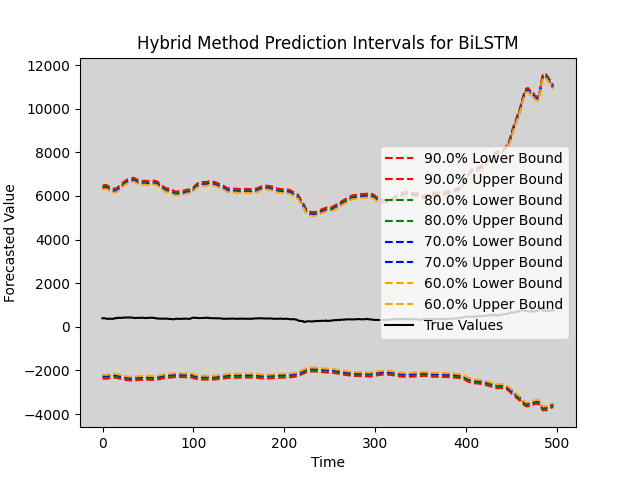
\includegraphics[width=\textwidth]{Chap03/figs/BiLSTM_hybrid_method_plot_AdaniPorts_Method2.png}
            \caption{BiLSTM.}
        \end{subfigure}
        \hfill
        \begin{subfigure}[b]{\textwidth}
            \centering
            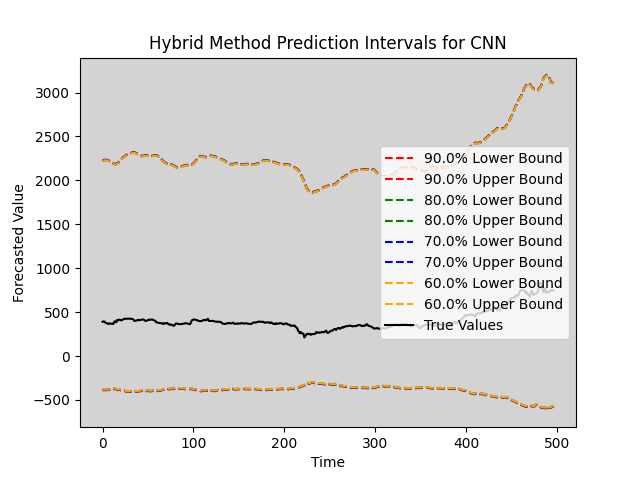
\includegraphics[width=\textwidth]{Chap03/figs/CNN_hybrid_method_plot_AdaniPorts_Method2.png}
            \caption{CNN.}
        \end{subfigure}
        \begin{subfigure}[b]{\textwidth}
            \centering
            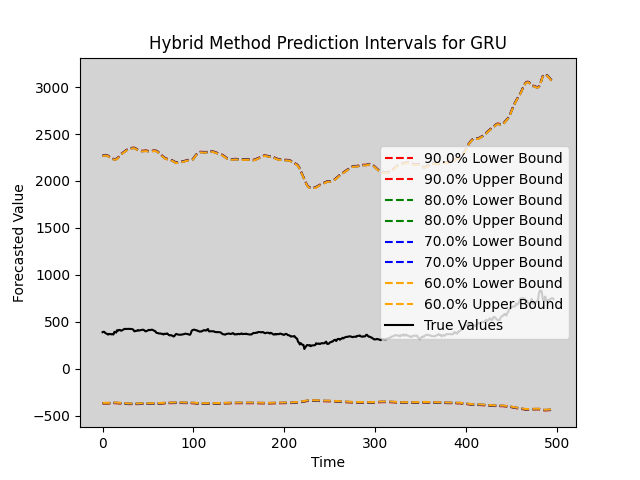
\includegraphics[width=\textwidth]{Chap03/figs/GRU_hybrid_method_plot_AdaniPorts_Method2.png}
            \caption{GRU.}
        \end{subfigure}
        \begin{subfigure}[b]{\textwidth}
            \centering
            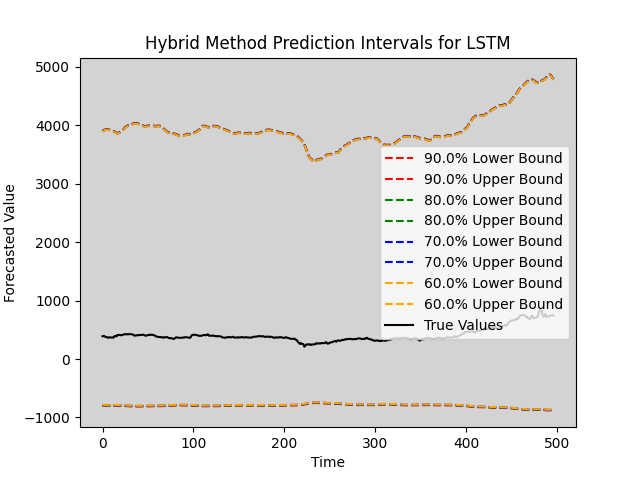
\includegraphics[width=\textwidth]{Chap03/figs/LSTM_hybrid_method_plot_AdaniPorts_Method2.png}
            \caption{LSTM.}
        \end{subfigure}
        \caption{Prediction Intervals for Adani Ports dataset obtained using proposed LUBE-Weibull based Hybrid Method and (a)BiLSTM, (b) CNN, (c) GRU, (d) LSTM Models.}
        \label{F 4.1}
    \end{minipage}
    \hfill
    \begin{minipage}{0.45\textwidth}
        \centering
        \begin{subfigure}[b]{\textwidth}
            \centering
            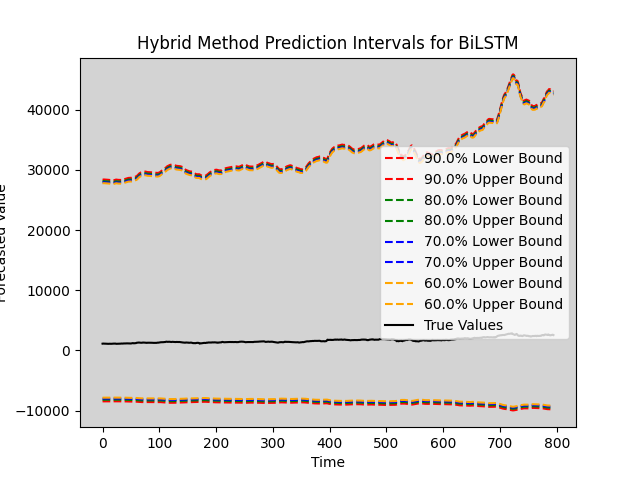
\includegraphics[width=\textwidth]{Chap03/figs/BiLSTM_hybrid_method_plot_AsianPaint_Method2.png}
            \caption{BiLSTM.}
        \end{subfigure}
        \hfill
        \begin{subfigure}[b]{\textwidth}
            \centering
            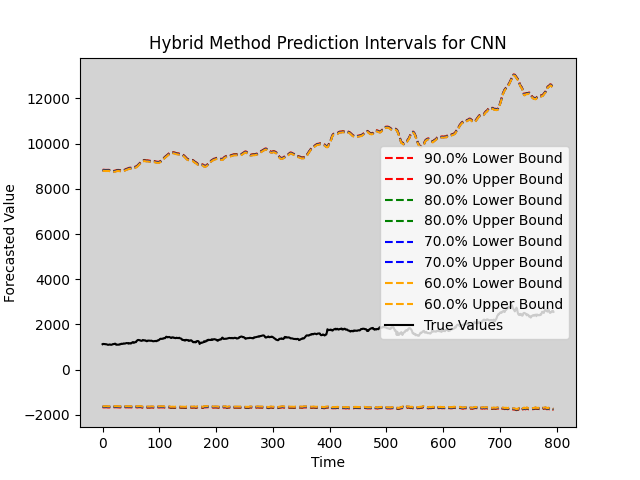
\includegraphics[width=\textwidth]{Chap03/figs/CNN_hybrid_method_plot_AsianPaint_Method2.png}
            \caption{CNN.}
        \end{subfigure}
        \begin{subfigure}[b]{\textwidth}
            \centering
            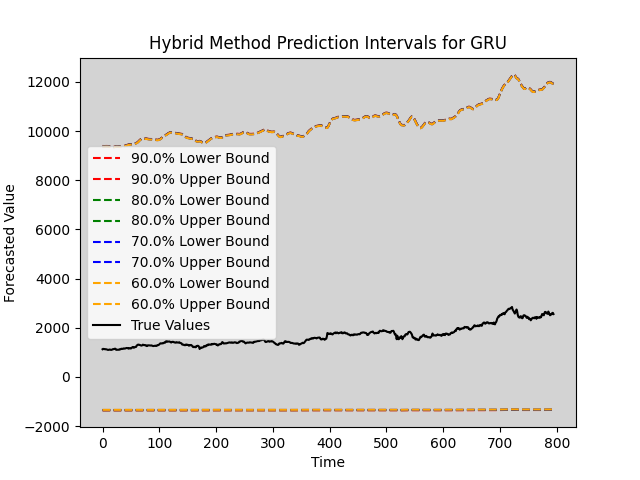
\includegraphics[width=\textwidth]{Chap03/figs/GRU_hybrid_method_plot_AsianPaint_Method2.png}
            \caption{GRU.}
        \end{subfigure}
        \begin{subfigure}[b]{\textwidth}
            \centering
            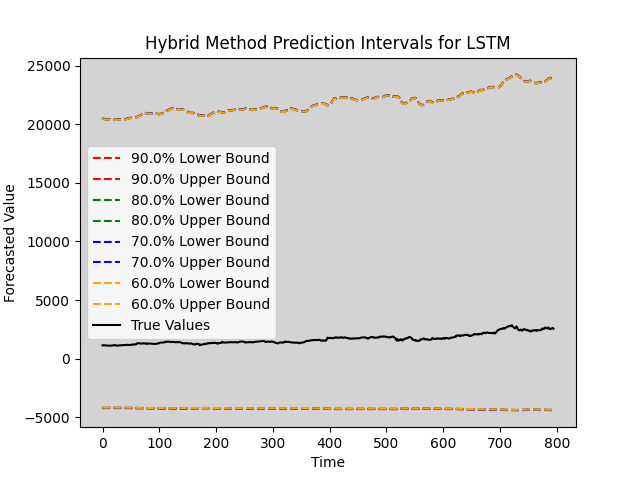
\includegraphics[width=\textwidth]{Chap03/figs/LSTM_hybrid_method_plot_AsianPaint_Method2.png}
            \caption{LSTM.}
        \end{subfigure}
        \caption{Prediction Intervals for Asian Paints dataset obtained using proposed LUBE-Weibull based Hybrid Method and (a)BiLSTM, (b) CNN, (c) GRU, (d) LSTM Models.}
        \label{F 4.2}
    \end{minipage}
\end{figure}


\begin{figure}[H]
    \centering
    \begin{minipage}{0.45\textwidth}
        \centering
        \begin{subfigure}[b]{\textwidth}
            \centering
            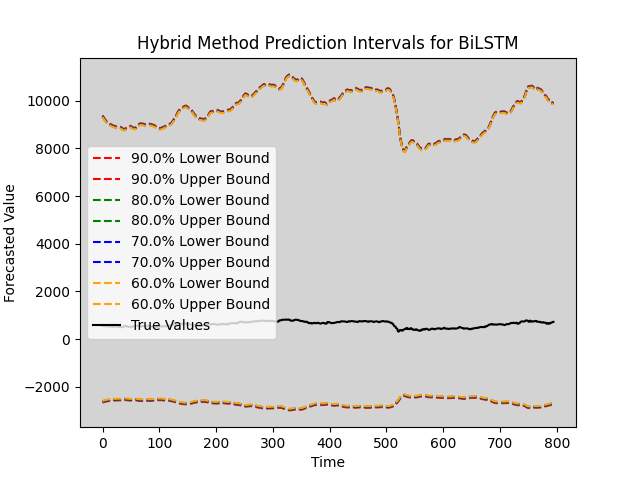
\includegraphics[width=\textwidth]{Chap03/figs/BiLSTM_hybrid_method_plot_AxisBank_Method2.png}
            \caption{BiLSTM.}
        \end{subfigure}
        \hfill
        \begin{subfigure}[b]{\textwidth}
            \centering
            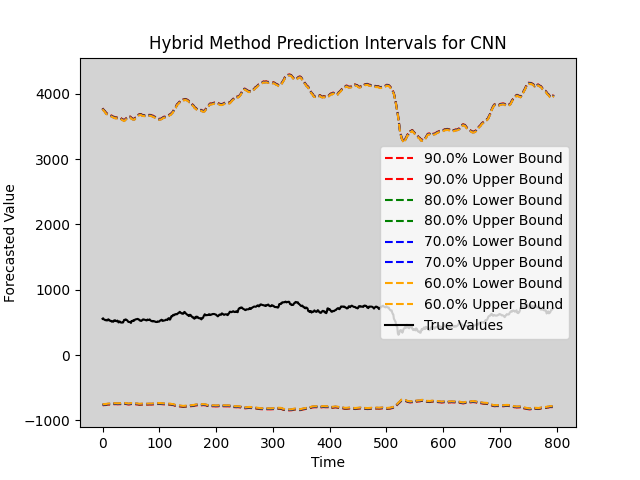
\includegraphics[width=\textwidth]{Chap03/figs/CNN_hybrid_method_plot_AxisBank_Method2.png}
            \caption{CNN.}
        \end{subfigure}
        \begin{subfigure}[b]{\textwidth}
            \centering
            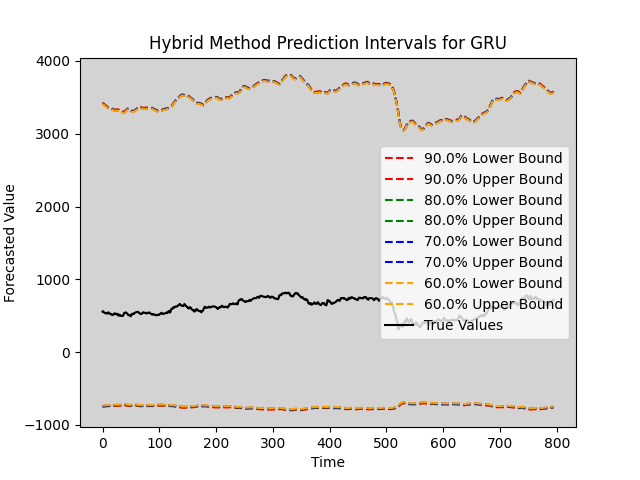
\includegraphics[width=\textwidth]{Chap03/figs/GRU_hybrid_method_plot_AxisBank_Method2.png}
            \caption{GRU.}
        \end{subfigure}
        \begin{subfigure}[b]{\textwidth}
            \centering
            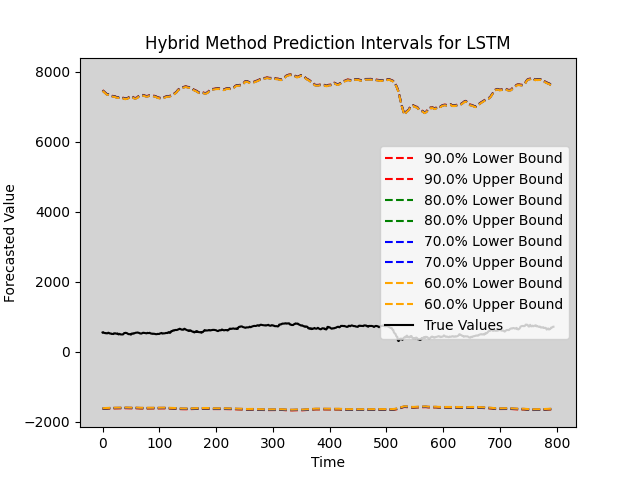
\includegraphics[width=\textwidth]{Chap03/figs/LSTM_hybrid_method_plot_AxisBank_Method2.png}
            \caption{LSTM.}
        \end{subfigure}
        \caption{Prediction Intervals for Axis Bank dataset obtained using proposed LUBE-Weibull based Hybrid Method and (a)BiLSTM, (b) CNN, (c) GRU, (d) LSTM Models.}
        \label{F 4.3}
    \end{minipage}
    \hfill
    \begin{minipage}{0.45\textwidth}
        \centering
        \begin{subfigure}[b]{\textwidth}
            \centering
            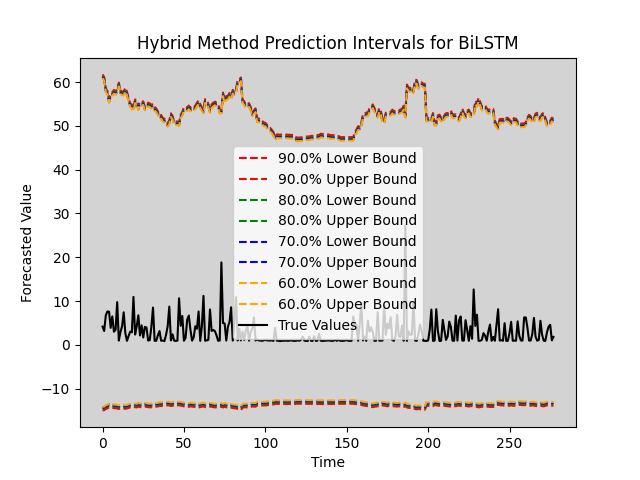
\includegraphics[width=\textwidth]{Chap03/figs/BiLSTM_hybrid_method_plot_Electricity_Consumption_Method2.png}
            \caption{BiLSTM.}
        \end{subfigure}
        \hfill
        \begin{subfigure}[b]{\textwidth}
            \centering
            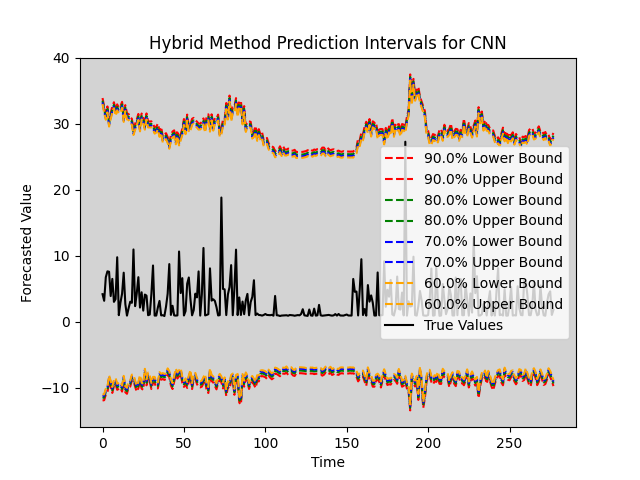
\includegraphics[width=\textwidth]{Chap03/figs/CNN_hybrid_method_plot_Electricity_Consumption_Method2.png}
            \caption{CNN.}
        \end{subfigure}
        \begin{subfigure}[b]{\textwidth}
            \centering
            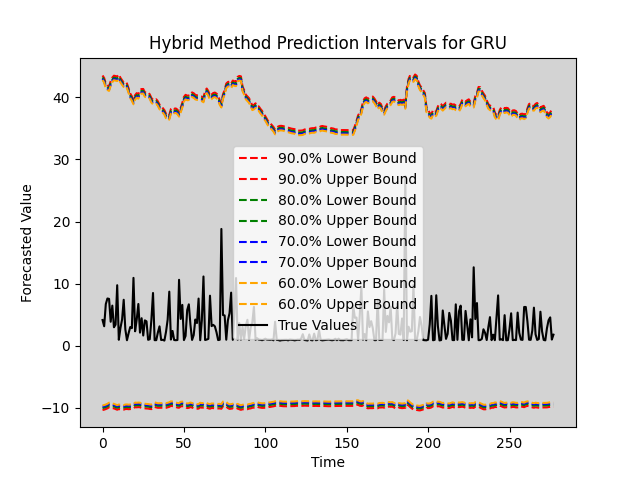
\includegraphics[width=\textwidth]{Chap03/figs/GRU_hybrid_method_plot_Electricity_Consumption_Method2.png}
            \caption{GRU.}
        \end{subfigure}
        \begin{subfigure}[b]{\textwidth}
            \centering
            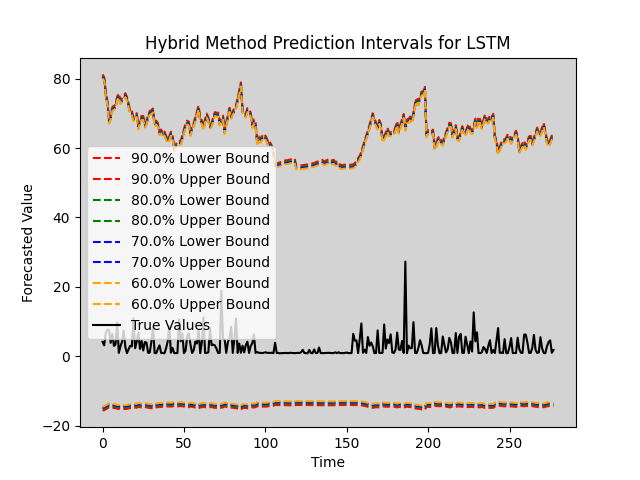
\includegraphics[width=\textwidth]{Chap03/figs/LSTM_hybrid_method_plot_Electricity_Consumption_Method2.png}
            \caption{LSTM.}
        \end{subfigure}
        \caption{Prediction Intervals for Electricity Consumption dataset obtained using proposed LUBE-Weibull based Hybrid Method and (a)BiLSTM, (b) CNN, (c) GRU, (d) LSTM Models.}
        \label{F 4.4}
    \end{minipage}
\end{figure}

\begin{figure}[H]
    \centering
        \begin{minipage}{0.4\textwidth}
            \centering
            \begin{subfigure}[b]{\textwidth}
                \centering
                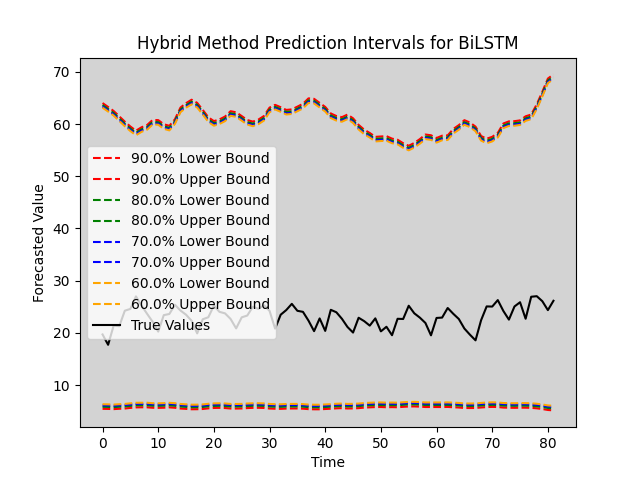
\includegraphics[width=\textwidth]{Chap03/figs/BiLSTM_hybrid_method_plot_Web_Traffic_Dataset_Method2.png}
                \caption{BiLSTM.}
            \end{subfigure}
            \hfill
            \begin{subfigure}[b]{\textwidth}
                \centering
                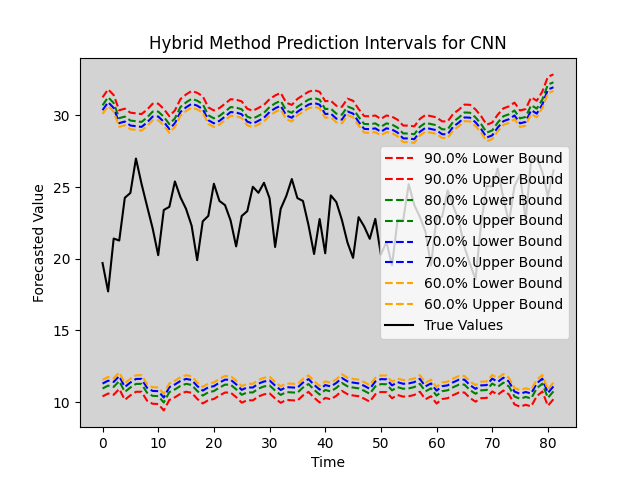
\includegraphics[width=\textwidth]{Chap03/figs/CNN_hybrid_method_plot_Web_Traffic_Dataset_Method2.png}
                \caption{CNN.}
            \end{subfigure}
            \begin{subfigure}[b]{\textwidth}
                \centering
                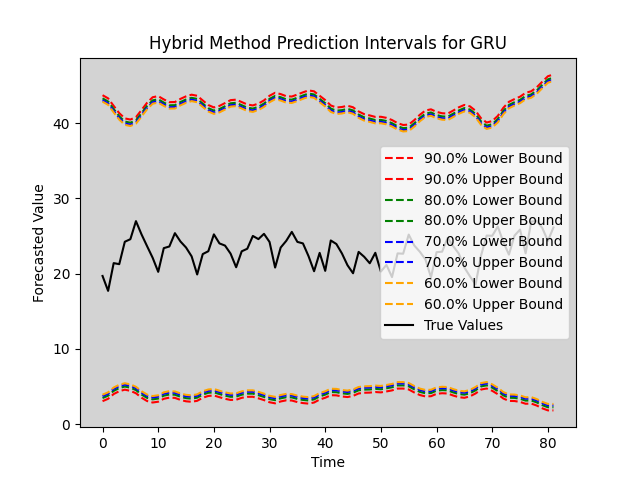
\includegraphics[width=\textwidth]{Chap03/figs/GRU_hybrid_method_plot_Web_Traffic_Dataset_Method2.png}
                \caption{GRU.}
            \end{subfigure}
            \begin{subfigure}[b]{\textwidth}
                \centering
                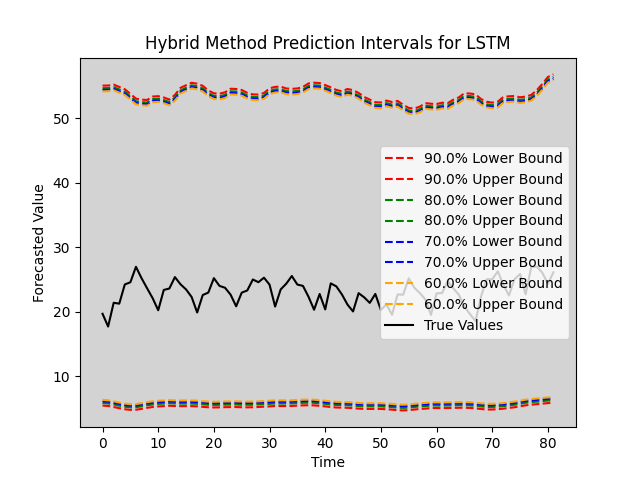
\includegraphics[width=\textwidth]{Chap03/figs/LSTM_hybrid_method_plot_Web_Traffic_Dataset_Method2.png}
                \caption{LSTM.}
            \end{subfigure}
        \end{minipage}
    
    \caption{Prediction Intervals for Web Traffic dataset obtained using proposed LUBE-Weibull based Hybrid Method and (a)BiLSTM, (b) CNN, (c) GRU, (d) LSTM Models.}
    \label{F 4.5}
\end{figure}

\begin{table*}[!t]
%\centering
\caption{Performance of LUBE-Weibull Hybrid Method on Adani Ports dataset.}
\vspace{0.5cm}
\renewcommand{\arraystretch}{1} % Adjust the value as needed
\resizebox{\textwidth}{!}{%
\begin{tabular}{|l|l|l|l|l|l|l|}
\hline
\textbf{Method Used} & \textbf{Confidence Level} & \textbf{Model} & \textbf{Avg PICP} & \textbf{Avg PINAW} &  \textbf{Avg ACE} & \textbf{Avg AWE} \\ \hline
\multirow{LUBE-Weibull Hybrid Method} 
& 0.6 & BiLSTM & 100 & 9.01 & 40 &  4995.50 \\ \cline{2-7}
& 0.6 & CNN & 100 & 4.15 & 40 & 1961.88 \\ \cline{2-7}
& 0.6 & GRU & 100 & 4.17 & 40 & 1979.80 \\ \cline{2-7}
& 0.6 & LSTM & 100 & 7.76 & 40 & 4218.70 \\ \cline{2-7}
& 0.7 & BiLSTM & 100 & 9.08 & 30 & 5039.80 \\ \cline{2-7}
& 0.7 & CNN & 100 & 4.16 & 30 & 1968.03 \\  \cline{2-7}
& 0.7 & GRU & 100 & 4.18 & 30 & 1984.13 \\ \cline{2-7}
& 0.7 & LSTM & 100 & 7.78 & 30 & 4227.40 \\ \cline{2-7}
& 0.8 & BiLSTM & 100 & 9.17 & 20 & 5093.81 \\ \cline{2-7}
& 0.8 & CNN & 100 & 4.17 & 20 & 1975.35 \\ \cline{2-7}
& 0.8 & GRU & 100 & 4.19 & 20 & 1989.29 \\ \cline{2-7}
& 0.8 & LSTM & 100 & 7.80 & 20 & 4237.76 \\ \cline{2-7}
& 0.9 & BiLSTM & 100 & 9.29 & 10 & 5170.50 \\ \cline{2-7}
& 0.9 & CNN & 100 & 4.18 & 10 & 1985.47 \\ \cline{2-7}
& 0.9 & GRU & 100 & 4.20 & 10 & 1996.40 \\ \cline{2-7}
& 0.9 & LSTM & 100 & 7.81 & 10 & 4252.00 \\ \hline
\end{tabular}%
}
\label{Table 3.1}
\end{table*}

\begin{table*}[!t]
%\centering
\caption{Performance of LUBE-Weibull Hybrid Method on Asian Paints dataset.}
\vspace{0.5cm}
\renewcommand{\arraystretch}{1} % Adjust the value as needed
\resizebox{\textwidth}{!}{%
\begin{tabular}{|l|l|l|l|l|l|l|}
\hline
\textbf{Method Used} & \textbf{Confidence Level} & \textbf{Model} & \textbf{Avg PICP} & \textbf{Avg PINAW} &  \textbf{Avg ACE} & \textbf{Avg AWE} \\ \hline
\multirow{LUBE-Weibull Hybrid Method} 
& 0.6 & BiLSTM & 100 & 23.37 & 40 & 39072.46 \\ \cline{2-7}
& 0.6 & CNN & 100 & 6.84 & 40 & 10198.06 \\ \cline{2-7}
& 0.6 & GRU & 100 & 7.41 & 40 & 11189.72 \\ \cline{2-7}
& 0.6 & LSTM & 100 & 15.27 & 40 & 24928.48 \\ \cline{2-7}
& 0.7 & BiLSTM & 100 & 23.56 & 30 & 39400.89 \\ \cline{2-7}
& 0.7 & CNN & 100 & 6.85 & 30 & 10219.74 \\ \cline{2-7}
& 0.7 & GRU & 100 & 7.42 & 30 & 11206.59 \\ \cline{2-7}
& 0.7 & LSTM & 100 & 15.28 & 30 & 24950.86 \\ \cline{2-7}
& 0.8 & BiLSTM & 100 & 23.78 & 20 & 39800.18 \\ \cline{2-7}
& 0.8 & CNN & 100 & 6.87 & 20 & 10245.51 \\ \cline{2-7}
& 0.8 & GRU & 100 & 7.43 & 20 & 11226.99 \\ \cline{2-7}
& 0.8 & LSTM & 100 & 15.30 & 20 & 24977.32 \\ \cline{2-7}
& 0.9 & BiLSTM & 100 & 24.11 & 10 & 40365.09 \\ \cline{2-7}
& 0.9 & CNN & 100 & 6.89 & 10 & 10280.97 \\ \cline{2-7}
& 0.9 & GRU & 100 & 7.44 & 10 & 11255.71 \\ \cline{2-7}
& 0.9 & LSTM & 100 & 15.32 & 10 & 25013.46 \\ \hline
\end{tabular}%
}
\label{Table 3.2}
\end{table*}

\begin{table*}[!t]
%\centering
\caption{Performance of LUBE-Weibull Hybrid Method on Axis Bank dataset.}
\vspace{0.5cm}
\renewcommand{\arraystretch}{1} % Adjust the value as needed
\resizebox{\textwidth}{!}{%
\begin{tabular}{|l|l|l|l|l|l|l|}
\hline
\textbf{Method Used} & \textbf{Confidence Level} & \textbf{Model} & \textbf{Avg PICP} & \textbf{Avg PINAW} &  \textbf{Avg ACE} & \textbf{Avg AWE} \\ \hline
\multirow{LUBE-Weibull Hybrid Method} 
& 0.6 & BiLSTM & 100 & 25.69 & 40 & 12517.84 \\ \cline{2-7}
& 0.6 & CNN & 100 & 8.70 & 40 & 3905.90 \\ \cline{2-7}
& 0.6 & GRU & 100 & 9.38 & 40 & 4250.76 \\ \cline{2-7}
& 0.6 & LSTM & 100 & 20.32 & 40 & 9793.09 \\ \cline{2-7}
& 0.7 & BiLSTM & 100 & 25.78 & 30 & 12562.57 \\ \cline{2-7}
& 0.7 & CNN & 100 & 8.72 & 30 & 3914.95 \\ \cline{2-7}
& 0.7 & GRU & 100 & 9.40 & 30 & 4259.08 \\ \cline{2-7}
& 0.7 & LSTM & 100 & 20.34 & 30 & 9805.74 \\ \cline{2-7}
& 0.8 & BiLSTM & 100 & 25.89 & 20 & 12616.01 \\ \cline{2-7}
& 0.8 & CNN & 100 & 8.74 & 20 & 3925.73 \\ \cline{2-7}
& 0.8 & GRU & 100 & 9.42 & 20 & 4269.04 \\ \cline{2-7}
& 0.8 & LSTM & 100 & 20.37 & 20 & 9820.72 \\ \cline{2-7}
& 0.9 & BiLSTM & 100 & 26.03 & 10 & 12689.96 \\ \cline{2-7}
& 0.9 & CNN & 100 & 8.77 & 10 & 3940.60 \\ \cline{2-7}
& 0.9 & GRU & 100 & 9.45 & 10 & 4282.84 \\ \cline{2-7}
& 0.9 & LSTM & 100 & 20.41 & 10 & 9841.23 \\ \hline

\end{tabular}%
}
\label{Table 3.3}
\end{table*}

\begin{table*}[!t]
%\centering
\caption{Performance of LUBE-Weibull Hybrid Method on Electricity Consumption dataset.}
\vspace{0.5cm}
\renewcommand{\arraystretch}{1} % Adjust the value as needed
\resizebox{\textwidth}{!}{%
\begin{tabular}{|l|l|l|l|l|l|l|}
\hline
\textbf{Method Used} & \textbf{Confidence Level} & \textbf{Model} & \textbf{Avg PICP} & \textbf{Avg PINAW} &  \textbf{Avg ACE} & \textbf{Avg AWE} \\ \hline
\multirow{LUBE-Weibull Hybrid Method} 
& 0.6 & BiLSTM & 100 & 2.54 & 40 & 40.62 \\ \cline{2-7}
& 0.6 & CNN & 100 & 1.37 & 40 & 9.85 \\ \cline{2-7}
& 0.6 & GRU & 100 & 1.86 & 40 & 22.64 \\ \cline{2-7}
& 0.6 & LSTM & 100 & 2.84 & 40 & 48.53 \\ \cline{2-7}
& 0.7 & BiLSTM & 100 & 2.55 & 30 & 41.07 \\ \cline{2-7}
& 0.7 & CNN & 100 & 1.39 & 30 & 10.30 \\ \cline{2-7}
& 0.7 & GRU & 100 & 1.87 & 30 & 23.01 \\ \cline{2-7}
& 0.7 & LSTM & 100 & 2.86 & 30 & 49.06 \\ \cline{2-7}
& 0.8 & BiLSTM & 100 & 2.57 & 20 & 41.60 \\ \cline{2-7}
& 0.8 & CNN & 100 & 1.41 & 20 & 10.85 \\ \cline{2-7}
& 0.8 & GRU & 100 & 1.89 & 20 & 23.46 \\ \cline{2-7}
& 0.8 & LSTM & 100 & 2.88 & 20 & 49.71 \\ \cline{2-7}
& 0.9 & BiLSTM & 100 & 2.60 & 10 & 42.35 \\ \cline{2-7}
& 0.9 & CNN & 100 & 1.44 & 10 & 11.65 \\ \cline{2-7}
& 0.9 & GRU & 100 & 1.91 & 10 & 24.10 \\ \cline{2-7}
& 0.9 & LSTM & 100 & 2.91 & 10 & 50.61 \\ \hline
\end{tabular}%
}
\label{Table 3.4}
\end{table*}

\begin{table*}[!t]
%\centering
\caption{Performance of LUBE-Weibull Hybrid Method on Web Traffic dataset.}
\vspace{0.5cm}
\renewcommand{\arraystretch}{1} % Adjust the value as needed
\resizebox{\textwidth}{!}{%
\begin{tabular}{|l|l|l|l|l|l|l|}
\hline
\textbf{Method Used} & \textbf{Confidence Level} & \textbf{Model} & \textbf{Avg PICP} & \textbf{Avg PINAW} &  \textbf{Avg ACE} & \textbf{Avg AWE} \\ \hline
\multirow{LUBE-Weibull Hybrid Method} 
& 0.6 & BiLSTM & 100 & 6.04 & 40 & 46.91 \\ \cline{2-7}
& 0.6 & CNN & 100 & 2.16 & 40 & 10.82 \\ \cline{2-7}
& 0.6 & GRU & 100 & 3.65 & 40 & 24.64 \\ \cline{2-7}
& 0.6 & LSTM & 100 & 5.35 & 40 & 40.52 \\ \cline{2-7}
& 0.7 & BiLSTM & 100 & 6.09 & 30 & 47.37 \\ \cline{2-7}
& 0.7 & CNN & 100 & 2.21 & 30 & 11.27 \\ \cline{2-7}
& 0.7 & GRU & 100 & 3.70 & 30 & 25.11 \\ \cline{2-7}
& 0.7 & LSTM & 100 & 5.40 & 30 & 40.96 \\ \cline{2-7}
& 0.8 & BiLSTM & 100 & 6.15 & 20 & 47.94 \\ \cline{2-7}
& 0.8 & CNN & 100 & 2.27 & 20 & 11.86 \\ \cline{2-7}
& 0.8 & GRU & 100 & 3.76 & 20 & 25.73 \\ \cline{2-7}
& 0.8 & LSTM & 100 & 5.46 & 20 & 41.52 \\ \cline{2-7}
& 0.9 & BiLSTM & 100 & 6.24 & 10 & 48.76 \\ \cline{2-7}
& 0.9 & CNN & 100 & 2.37 & 10 & 12.79 \\ \cline{2-7}
& 0.9 & GRU & 100 & 3.87 & 10 & 26.69 \\ \cline{2-7}
& 0.9 & LSTM & 100 & 5.55 & 10 & 42.35 \\ \hline
\end{tabular}%
}
\label{Table 3.5}
\end{table*}
\clearpage

\subsection{Discussion}
The results demonstrate that the LUBE-Weibull Hybrid Method maintains 100\% PICP like the standalone LUBE method without compromising acceptable PINAW values. The ACE values reflect that the method achieves confidence levels that are essentially similar to the target measures. Additionally, the AWE values confirms that the Weibull-based adjustment prevents the over-broadening of prediction intervals.
We have certainly achieved better results than the traditional LUBE method while also significantly reducing the required time and computational requirements by incorporating the Weibull method.

The last section provides a summary of the research and suggests potential avenues for future research.

\section{Summary}
This chapter introduced the LUBE-Weibull Based Hybrid Approach to probabilistic time series forecasting, which integrates deep learning-driven prediction interval estimation with Weibull-based residual correction. Experimental results demonstrate that the hybrid approach outperforms the Traditional LUBE Method in terms of improving coverage probability (PICP) with an acceptable balance between interval sharpness (PINAW) and accuracy (ACE). Deployment of Weibull-based correction effectively sharpens prediction intervals by accounting for residual uncertainties, thus improving forecast reliability.

Comparison with the Advanced LUBE Method reveals that the hybrid approach has a marginally increased AWE, indicating slightly wider prediction intervals. However, this feature may offer a potential benefit: the Hybrid Method is computationally more efficient, as it removes extra complexity in the loss function while performing post-hoc corrections to sharpen interval estimation. This trade-off suggests that the Hybrid Method offers a viable and scalable alternative to Advanced LUBE, especially in situations requiring tradeoff between computational cost and forecasting quality.

Future research can explore adaptive scaling of Weibull corrections to further improve interval sharpness without compromising coverage. Moreover, the use of uncertainty-aware deep learning architectures or ensembling of heterogeneous architectures may potentially improve predictive quality.

\chapter{LUBE-QR Based Hybrid Method For Probabilistic Time Series Forecasting}\label{January Update}

\section{ Motivation}
Forecasting is very important in domains like energy, finance, healthcare, and climatology, as accurate predictions allow for well-informed and efficient decision making. While traditional forecasting methodologies tend to produce point estimates, they have the disadvantage of excluding uncertainty, an oversight that can lead to erroneous conclusions and inefficient use of resources, especially in risky scenarios. Probabilistic forecasting rectifies this by providing prediction intervals (PIs) that estimate uncertainty and allow for risk informed decision making. However, choice of the most appropriate method is a major problem. Parametric methods, including Gaussian and Weibull Distribution based methods, are computationally efficient but can fall short of capturing complex patterns in the data. Non-parametric methods, like Quantile Regression and Bootstrap-based methods are more data adaptive and versatile but are computationally demanding.

The Lower Upper Bound Estimation (LUBE) algorithm, a deep learning-based non-parametric algorithm, learns PIs from data but lacks reliability in highly dynamic environments. 
Weibull distribution modeling, in contrast, models residual errors accurately but lacks adaptability to time-dependent forecast changes.

This chapter presents the LUBE-QR Based Hybrid Method, a technique that improves PI reliability through the combination of deep learning-based LUBE prediction and QR-based residual correction. 

The technique consists of using deep learning models (LSTM, CNN, GRU, BiLSTM) to produce initial prediction intervals, and residual error modeling through QR method.
The QR-based corrections improve the intervals, which improves accuracy and stability at various confidence levels. 

Through the combination of the flexibility of deep learning and statistical error modeling, the technique presents stronger and more reliable probabilistic predictions. 


\section{Methodology}
\subsection{Data Pre-processing}
The time series datasets are preprocessed to ensure stable training and effective modeling. First, the data is normalized to the range [0,1] using MinMaxScaler. Next, a sliding window approach with a window size of 12 is applied to generate input-output pairs, where the past 12 time steps are used to predict the next step. Finally, the dataset is divided into three subsets: 70\% for training, 15\% for validation, and 15\% for testing, ensuring a balanced and robust evaluation of the model.

\subsection{Model Selection}
The hybrid method employs different deep learning architectures to generate first-stage prediction intervals (PIs). Long Short-Term Memory (LSTM) is well suited to learning long-term dependencies of sequential data, while Convolutional Neural Networks (CNN) are best at detecting local patterns and trends. Gated Recurrent Units (GRU) offer a computationally cheaper option that still retains the ability to learn sequences. Additionally, Bidirectional LSTM (BiLSTM) enhances feature extraction through learning information in both directions. Each model delivers two outputs for each prediction, which represent the lower and upper bounds of the PI and hence enable extensive estimation of uncertainty.

\subsection{LUBE Loss Function}
The LUBE method directly learns interval bounds using a custom loss function. The LUBE loss function is defined as:

\begin{equation}
\mathcal{L}_{\text{LUBE}} = \text{PINAW} + \lambda \cdot \max\left(0,\left(1 - \text{PICP}_{\text{target}}\right) - \text{PICP} \right)^2
\label{LUBE Loss Function}
\end{equation}

Where:
\begin{itemize}
    \item PINAW is Prediction Interval Normalized Average Width, which penalizes wide intervals.
    
    \item PICP is Prediction Interval Coverage Probability, representing the fraction of true values that lie within the predicted intervals.
    
    \item $\lambda$ is a regularization hyperparameter that controls the trade-off between narrow intervals and sufficient coverage.
    
    \item $UB_i$, $LB_i$ are the predicted upper and lower bounds for the $i^{\text{th}}$ data point.
    
    \item $y_i$ is the true value of the $i^{\text{th}}$ sample.
    
    \item $\text{PICP}_{\text{target}}$ is the desired confidence level, such as 0.9, 0.8, 0.7 or 0.6.
    
    \item R is the range of the training target values, used to normalize the interval width.
    
    \item $\mathbb{I}(\cdot)$ is the indicator function, which returns 1 if the condition inside is true, and 0 otherwise.
\end{itemize}

The loss aims to produce prediction intervals that are as narrow as possible (minimizing $\text{PINAW}$), while ensuring they capture the true target values with the desired coverage level (maximizing $\text{PICP}$).

\\

\subsection{QR-Based Residual Correction}

After generating initial prediction intervals $[LB_i, UB_i]$ using the Advanced LUBE method, the Hybrid LUBE–QR framework applies a correction based on quantile regression to refine the interval bounds using residual information.

Let the residuals be defined as:
\begin{equation}
r_i = |y_i - \hat{y}_i|
\label{residual}
\end{equation}
where $y_i$ is the true target value and $\hat{y}_i = \frac{LB_i + UB_i}{2}$ is the midpoint (mean prediction) of the LUBE interval.

A Quantile Regression (QR) model is then trained to estimate specific conditional quantiles of the residuals, denoted as $Q_{\tau}(r|x)$, where $\tau$ represents the desired quantile level (e.g., $\tau = 0.9, 0.95$). The model learns to predict asymmetric quantiles based on the input features $x$.

For a target confidence level $c$, we determine the corresponding quantile correction $\delta_c$ such that:
\begin{equation}
\delta_c = Q_{1 - \frac{1 - c}{2}}(r|x)
\label{quantile correction}
\end{equation}

The final corrected prediction interval is:
\begin{subequations} \label{eq:corrected_bounds}
\begin{align}
LB_i^{\text{corrected}} &= \hat{y}_i - \delta_c \\
UB_i^{\text{corrected}} &= \hat{y}_i + \delta_c
\end{align}
\end{subequations}


The Eq. \ref{quantile correction} shows the quantile correction formula while the Eq. \ref{eq:corrected_bounds} shows the corrected Lower Bound and Upper Bound obtained. This residual-based QR correction enables the prediction intervals to better account for heteroscedasticity and non-Gaussian uncertainty structures, resulting in intervals that are not only statistically valid but also adaptive to local data variability.
\\

\subsection{Confidence Levels and Performance Metrics}
The hybrid method examines prediction intervals for four confidence levels: 90\%, 80\%, 70\%, and 60\%, giving a complete uncertainty estimation evaluation. Performance is measured via several key indicators. Prediction Interval Coverage Probability (PICP) estimates the percentage of actual values in the predicted interval, assessing reliability. Prediction Interval Normalized Average Width (PINAW) estimates interval sharpness as a function of data range, sacrificing precision for coverage. Average Coverage Error (ACE) estimates PICP deviation from the target confidence level, measuring calibration accuracy. Lastly, Average Width Error (AWE) evaluates how far interval width is from expected bounds, ensuring proper uncertainty quantification.

\subsection{Probabilistic Forecasting using Hybrid LUBE-QR Based Method}
\begin{algorithm}
    \small
    %\normalsize
    \SetAlgoNlRelativeSize{0}
    \SetAlgoCaptionSeparator{:}
    
    \KwIn{Time series dataset $D$}
    \KwOut{Predicted intervals $[LB', UB']$, PICP, PINAW, ACE, AWE}
    
    \textbf{Step 1: Data Preprocessing}\\
    Normalize $D$ using MinMaxScaler\\
    Generate input-output pairs with window size $w$\\
    Split into train, validation, and test sets\\
    
    \textbf{Step 2: Define Advanced LUBE Loss}\\
    \ForEach{$c \in \{0.9, 0.8, 0.7, 0.6\}$}{
        $q = 1 - c$\\
        Compute $LB$, $UB$\\
        Compute $\text{Loss}_{\text{lower}}$\\
        Compute $\text{Loss}_{\text{upper}}$\\
        Compute PICP (as in Eq.~\eqref{Equation 1}) and PINAW (as in Eq.~\eqref{Equation 2})\\
        Compute $\text{Loss}_{\text{LUBE}}$ (as in Eq.~\eqref{LUBE Loss Function}).
    }
    
    \textbf{Step 3: Model Training}\\
    \ForEach{$M \in \{$LSTM, CNN, GRU, BiLSTM$\}$}{
        Define model architecture\\
        Compile with Advanced LUBE loss\\
        Train on $(X_{\text{train}}, y_{\text{train}})$ for $e$ epochs\\
        Validate on $(X_{\text{val}}, y_{\text{val}})$\\
        Predict LUBE bounds $LB, UB$ on test data\\
        Compute midpoint $\hat{y}$
    }
    
    \textbf{Step 4: Fit Quantile Regression on Residuals}\\
    Compute residuals (as in Eq. \eqref{residual})\\
    \ForEach{$c \in \{0.9, 0.8, 0.7, 0.6\}$}{
        Train Quantile Regression models to estimate:\\
        Lower quantile and Upper quantile\\
        Predict residual quantiles $\hat{r}_{\text{lower}}, \hat{r}_{\text{upper}}$\\
    }
    
    \textbf{Step 5: Adjust Prediction Intervals Using QR Correction}\\
    \ForEach{$c \in \{0.9, 0.8, 0.7, 0.6\}$}{
        $LB' = \hat{y} + \hat{r}_{\text{lower}}$\\
        $UB' = \hat{y} + \hat{r}_{\text{upper}}$\\
    }

    \textbf{Step 6: Evaluation Metrics} Compute the PICP (as in Eq.~\eqref{Equation 1}), PINAW (as in Eq. ~\eqref{Equation 2}), ACE (as in Eq. ~\eqref{Equation 3}) and AWE (as in Eq. ~\eqref{Equation 4}) of the computed prediction intervals.

    
    \textbf{Step 7: Aggregate Results}\\
    \text{Compute mean of metrics for each case}\\
    
    \caption{Hybrid LUBE–QR Method.}
\end{algorithm}

The crux of this algorithm begins with training deep-learning models (LSTM, BiLSTM, CNN, GRU) on a tailored LUBE loss function that is specifically tailored to optimize interval width and violation of coverage. For each pre-specified confidence level (0.6, 0.7, 0.8, 0.9), the LUBE loss is dynamically scaled to penalize the failure of prediction intervals to cover the true values. This training produces initial lower and upper bounds for the target variable, which are the initial prediction intervals.

Lastly, the method estimates the midpoint of the LUBE-generated intervals and the absolute residuals between the predicted midpoint and observed target values are estimated. These residuals are the systematic forecasting errors not explained by the original model. Quantile Regression is applied to the residuals to estimate the lower and upper quantiles at each confidence level. This helps to model the residual distribution in a non-parametric and data-adaptive manner. The quantile forecasts are subsequently combined with the forecasted midpoint to provide improved lower and upper limits for the final prediction intervals. The two-stage adjustment process enables the model to improve its interval estimates by exploiting both interval-targeted loss optimization and quantile-based residual learning.

For each run and model, the following metrics are computed for each run and model to measure the quality of the prediction intervals: Prediction Interval Coverage Probability (PICP), Prediction Interval Normalized Average Width (PINAW), Average Coverage Error (ACE) and Absolute Width Error (AWE). The whole process is repeated for 10 independent runs for all types of models and confidence levels to provide statistical robustness. Finally, the results are aggregated and saved in structured CSV formats, and graphical visualizations are generated for all models, showing the predicted intervals over the test data for different confidence levels.

%\newpage
\section{Results and Discussions}
This section displays the evaluation of the LUBE-QR Based Hybrid Method across five datasets. The performance of the hybrid approach is assessed using metrics PICP, PINAW, ACE and AWE. The results are visualized through prediction interval plots and summarized in tables.\\ 

Figures \ref{fig 5.1}, \ref{fig 5.2}, \ref{fig 5.3}, \ref{fig 5.4} and \ref{fig 5.5} shows Prediction Intervals for all the five different datasets obtained using proposed LUBE-QR based Hybrid Method and (a) BiLSTM, (b) CNN, (c) GRU, (d) LSTM Models respectively.\\

Tables \ref{table 5.1}, \ref{table 5.2}, \ref{table 5.3}, \ref{table 5.4} and \ref{table 5.5} shows the performance of the proposed LUBE-QR based Hybrid Method on all the five datasets respectively across the four metrics PICP, PINAW, ACE and AWE for four different confidence levels 60\%, 70\%, 80\% and 90\%.\\

It is visible from Figures \ref{fig 5.1} to \ref{fig 5.5} and from Tables \ref{table 5.1} to \ref{table 5.5} that the results obtained from this Hybrid LUBE-QR method produces crisp and sharp intervals while maintaining low values of PINAW, ACE and AWE. This makes this hybrid model a good alternative to existing traditional models for real time probabilistic forecasting tasks.

\subsection{Visualization Of Prediction Intervals}

\begin{figure}[H]
    \centering
    \begin{minipage}{0.49\textwidth}
        \centering
        \begin{subfigure}[b]{\textwidth}
            \centering
            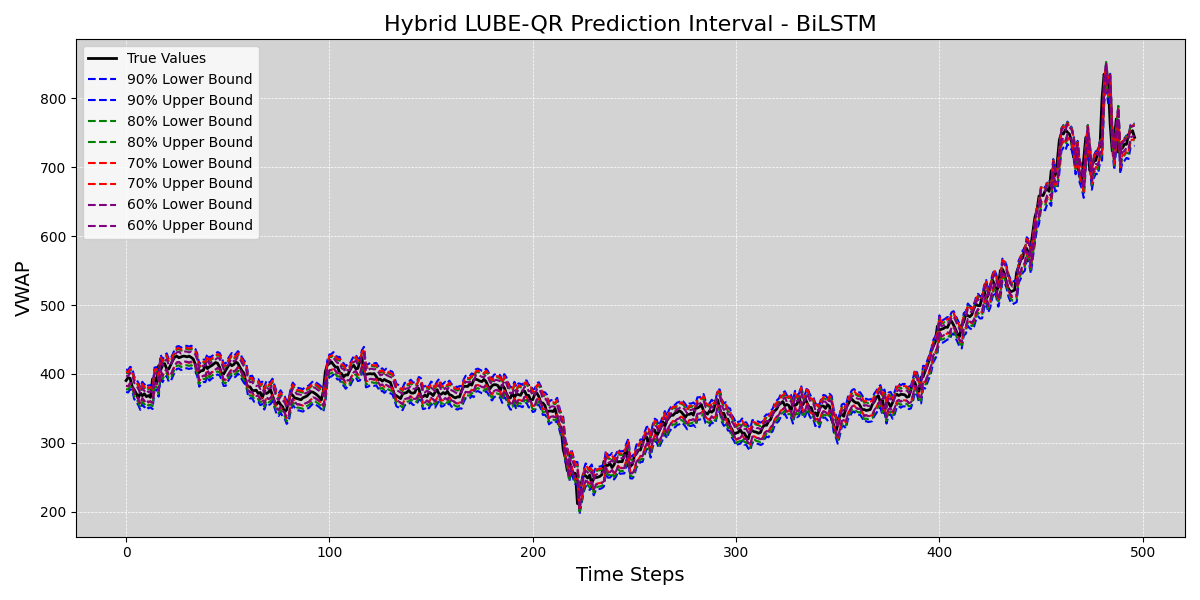
\includegraphics[width=\textwidth]{Chap03/figs/AP_Hybrid_LUBE_QR_AllConfidence_BiLSTM.png}
            \caption{BiLSTM.}
        \end{subfigure}
        \hfill
        \begin{subfigure}[b]{\textwidth}
            \centering
            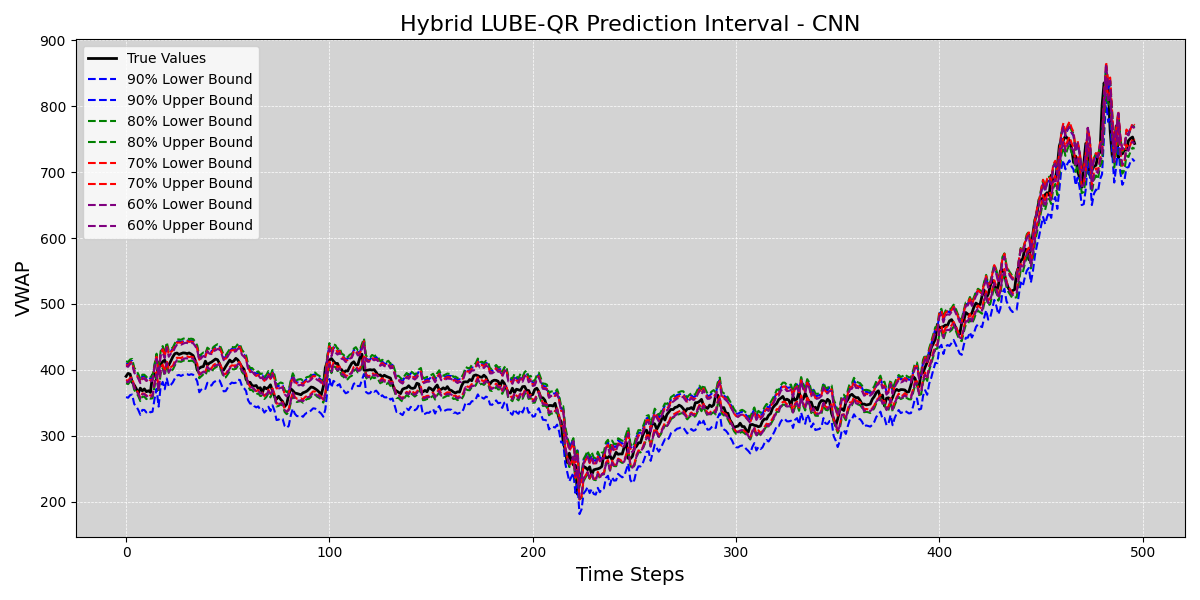
\includegraphics[width=\textwidth]{Chap03/figs/AP_Hybrid_LUBE_QR_AllConfidence_CNN.png}
            \caption{CNN.}
        \end{subfigure}
        \begin{subfigure}[b]{\textwidth}
            \centering
            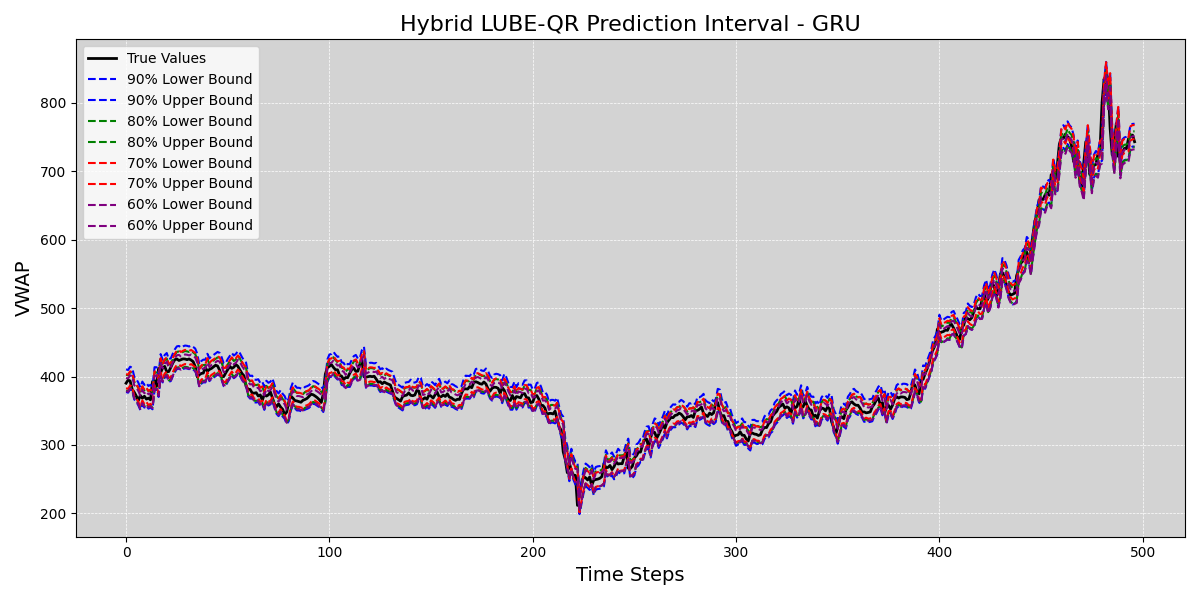
\includegraphics[width=\textwidth]{Chap03/figs/AP_Hybrid_LUBE_QR_AllConfidence_GRU.png}
            \caption{GRU.}
        \end{subfigure}
        \begin{subfigure}[b]{\textwidth}
            \centering
            \includegraphics[width=\textwidth]{Chap03/figs/AP_Hybrid_LUBE_QR_AllConfidence_LSTM.png}
            \caption{LSTM.}
        \end{subfigure}
        \caption{Prediction Intervals for Adani Ports dataset obtained using proposed LUBE-QR based Hybrid Method and (a) BiLSTM, (b) CNN, (c) GRU, (d) LSTM Models respectively.}
        \label{fig 5.1}
    \end{minipage}
    \hfill
    \begin{minipage}{0.49\textwidth}
        \centering
        \begin{subfigure}[b]{\textwidth}
            \centering
            \includegraphics[width=\textwidth]{Chap03/figs/AsianPaint_Hybrid_LUBE_QR_AllConfidence_BiLSTM.png}
            \caption{BiLSTM.}
        \end{subfigure}
        \hfill
        \begin{subfigure}[b]{\textwidth}
            \centering
            \includegraphics[width=\textwidth]{Chap03/figs/AsianPaint_Hybrid_LUBE_QR_AllConfidence_CNN.png}
            \caption{CNN.}
        \end{subfigure}
        \begin{subfigure}[b]{\textwidth}
            \centering
            \includegraphics[width=\textwidth]{Chap03/figs/AsianPaint_Hybrid_LUBE_QR_AllConfidence_GRU.png}
            \caption{GRU.}
        \end{subfigure}
        \begin{subfigure}[b]{\textwidth}
            \centering
            \includegraphics[width=\textwidth]{Chap03/figs/AsianPaint_Hybrid_LUBE_QR_AllConfidence_LSTM.png}
            \caption{LSTM.}
        \end{subfigure}
        \caption{Prediction Intervals for Asian Paints dataset obtained using proposed LUBE-QR based Hybrid Method and (a) BiLSTM, (b) CNN, (c) GRU, (d) LSTM Models respectively.}
        \label{fig 5.2}
    \end{minipage}
\end{figure}


\begin{figure}[H]
    \centering
    \begin{minipage}{0.49\textwidth}
        \centering
        \begin{subfigure}[b]{\textwidth}
            \centering
            \includegraphics[width=\textwidth]{Chap03/figs/Hybrid_LUBE_QR_AllConfidence_axisbank_BiLSTM.png}
            \caption{BiLSTM.}
        \end{subfigure}
        \hfill
        \begin{subfigure}[b]{\textwidth}
            \centering
            \includegraphics[width=\textwidth]{Chap03/figs/Hybrid_LUBE_QR_AllConfidence_axisbank_CNN.png}
            \caption{CNN.}
        \end{subfigure}
        \begin{subfigure}[b]{\textwidth}
            \centering
            \includegraphics[width=\textwidth]{Chap03/figs/Hybrid_LUBE_QR_AllConfidence_axisbank_GRU.png}
            \caption{GRU.}
        \end{subfigure}
        \begin{subfigure}[b]{\textwidth}
            \centering
            \includegraphics[width=\textwidth]{Chap03/figs/Hybrid_LUBE_QR_AllConfidence_axisbank_LSTM.png}
            \caption{LSTM.}
        \end{subfigure}
        \caption{Prediction Intervals for Axis Bank dataset obtained using proposed LUBE-QR based Hybrid Method and (a) BiLSTM, (b) CNN, (c) GRU, (d) LSTM Models respectively.}
        \label{fig 5.3}
    \end{minipage}
    \hfill
    \begin{minipage}{0.49\textwidth}
        \centering
        \begin{subfigure}[b]{\textwidth}
            \centering
            \includegraphics[width=\textwidth]{Chap03/figs/Hybrid_LUBE_QR_AllConfidence_elec_consumption_BiLSTM.png}
            \caption{BiLSTM.}
        \end{subfigure}
        \hfill
        \begin{subfigure}[b]{\textwidth}
            \centering
            \includegraphics[width=\textwidth]{Chap03/figs/Hybrid_LUBE_QR_AllConfidence_elec_consumption_GRU.png}
            \caption{CNN.}
        \end{subfigure}
        \begin{subfigure}[b]{\textwidth}
            \centering
            \includegraphics[width=\textwidth]{Chap03/figs/Hybrid_LUBE_QR_AllConfidence_elec_consumption_GRU.png}
            \caption{GRU.}
        \end{subfigure}
        \begin{subfigure}[b]{\textwidth}
            \centering
            \includegraphics[width=\textwidth]{Chap03/figs/Hybrid_LUBE_QR_AllConfidence_elec_consumption_BiLSTM.png}
            \caption{LSTM.}
        \end{subfigure}
        \caption{Prediction Intervals for Electricity Consumption dataset obtained using proposed LUBE-QR based Hybrid Method and (a) BiLSTM, (b) CNN, (c) GRU, (d) LSTM Models respectively.}
        \label{fig 5.4}
    \end{minipage}
\end{figure}

\begin{figure}[H]
    \centering
        \begin{minipage}{0.50\textwidth}
            \centering
            \begin{subfigure}[b]{\textwidth}
                \centering
                \includegraphics[width=\textwidth]{Chap03/figs/Hybrid_LUBE_QR_AllConfidence_web_traffic_BiLSTM.png}
                \caption{BiLSTM.}
            \end{subfigure}
            \hfill
            \begin{subfigure}[b]{\textwidth}
                \centering
                \includegraphics[width=\textwidth]{Chap03/figs/Hybrid_LUBE_QR_AllConfidence_web_traffic_CNN.png}
                \caption{CNN.}
            \end{subfigure}
            \begin{subfigure}[b]{\textwidth}
                \centering
                \includegraphics[width=\textwidth]{Chap03/figs/Hybrid_LUBE_QR_AllConfidence_web_traffic_GRU.png}
                \caption{GRU.}
            \end{subfigure}
            \begin{subfigure}[b]{\textwidth}
                \centering
                \includegraphics[width=\textwidth]{Chap03/figs/Hybrid_LUBE_QR_AllConfidence_web_traffic_LSTM.png}
                \caption{LSTM.}
            \end{subfigure}
        \end{minipage}
    
    \caption{Prediction Intervals for Web Traffic Load dataset obtained using proposed LUBE-QR based Hybrid Method and (a) BiLSTM, (b) CNN, (c) GRU, (d) LSTM Models respectively.}
    \label{fig 5.5}
\end{figure}
\clearpage

\begin{table*}[!t]
%\centering
\caption{Performance of LUBE-QR Hybrid Method on Adani Ports dataset.}
\vspace{0.5cm}
\renewcommand{\arraystretch}{1} % Adjust the value as needed
\resizebox{\textwidth}{!}{%
\begin{tabular}{|l|l|l|l|l|l|l|}
\hline
\textbf{Method Used} & \textbf{Confidence Level} & \textbf{Model} & \textbf{Avg PICP} & \textbf{Avg PINAW} &  \textbf{Avg ACE} & \textbf{Avg AWE} \\ \hline
\multirow{LUBE-QR Hybrid Method} 
& 0.6 & BiLSTM & 59.96 & 0.02 & 0.04 & 608.92  \\ \cline{2-7}
& 0.6 & CNN & 59.96 & 0.04 & 0.04 & 600.10 \\ \cline{2-7}
& 0.6 & GRU & 59.96 & 0.03 & 0.04 & 604.20 \\ \cline{2-7}
& 0.6 & LSTM & 59.96 & 0.02 & 0.04 & 608.53 \\ \cline{2-7}
& 0.7 & BiLSTM & 70.02 & 0.03 & 0.02 & 602.85 \\ \cline{2-7}
& 0.7 & CNN & 70.02 & 0.04 & 0.02 & 600.50 \\  \cline{2-7}
& 0.7 & GRU & 70.02 & 0.03 & 0.02 & 602.87 \\ \cline{2-7}
& 0.7 & LSTM & 70.02 & 0.03 & 0.02 & 602.49 \\ \cline{2-7}
& 0.8 & BiLSTM & 79.88 & 0.04 & 0.12 & 599.96 \\ \cline{2-7}
& 0.8 & CNN & 79.88 & 0.05 & 0.12 & 590.15 \\ \cline{2-7}
& 0.8 & GRU & 79.88 & 0.04 & 0.12 & 600.54 \\ \cline{2-7}
& 0.8 & LSTM & 79.88 & 0.05 & 0.12 & 593.65 \\ \cline{2-7}
& 0.9 & BiLSTM & 89.94 & 0.05 & 0.06 & 591.02 \\ \cline{2-7}
& 0.9 & CNN & 89.94 & 0.08 & 0.06 & 572.53 \\ \cline{2-7}
& 0.9 & GRU & 89.94 & 0.05 & 0.06 & 590.39 \\ \cline{2-7}
& 0.9 & LSTM & 89.94 & 0.06 & 0.06 & 583.94 \\ \hline
\end{tabular}%
}
\label{table 5.1}
\end{table*}

\begin{table*}[!t]
%\centering
\caption{Performance of LUBE-QR Hybrid Method on Asian Paints dataset.}
\vspace{0.5cm}
\renewcommand{\arraystretch}{1} % Adjust the value as needed
\resizebox{\textwidth}{!}{%
\begin{tabular}{|l|l|l|l|l|l|l|}
\hline
\textbf{Method Used} & \textbf{Confidence Level} & \textbf{Model} & \textbf{Avg PICP} & \textbf{Avg PINAW} &  \textbf{Avg ACE} & \textbf{Avg AWE} \\ \hline
\multirow{LUBE-QR Hybrid Method} 
& 0.6 & BiLSTM & 60.00 & 0.04 & 0.00 & 1679.25 \\ \cline{2-7}
& 0.6 & CNN & 60.00 & 0.05 & 0.00 & 1660.44 \\ \cline{2-7}
& 0.6 & GRU & 60.00 & 0.02 & 0.00 & 1704.50 \\ \cline{2-7}
& 0.6 & LSTM & 60.00 & 0.06 & 0.00 & 1639.36 \\ \cline{2-7}
& 0.7 & BiLSTM & 69.94 & 0.03 & 0.06 & 1687.10 \\ \cline{2-7}
& 0.7 & CNN & 69.94 & 0.04 & 0.06 & 1668.43 \\ \cline{2-7}
& 0.7 & GRU & 69.94 & 0.04 & 0.06 & 1675.49 \\ \cline{2-7}
& 0.7 & LSTM & 69.94 & 0.04 & 0.06 & 1670.81 \\ \cline{2-7}
& 0.8 & BiLSTM & 80.00 & 0.04 & 0.00 & 1679.75 \\ \cline{2-7}
& 0.8 & CNN & 80.00 & 0.05 & 0.00 & 1659.36 \\ \cline{2-7}
& 0.8 & GRU & 80.00 & 0.04 & 0.00 & 1685.31 \\ \cline{2-7}
& 0.8 & LSTM & 80.00 & 0.05 & 0.00 & 1662.02 \\ \cline{2-7}
& 0.9 & BiLSTM & 89.94 & 0.08 & 0.06 & 1603.47 \\ \cline{2-7}
& 0.9 & CNN & 89.94 & 0.08 & 0.06 & 1608.31 \\ \cline{2-7}
& 0.9 & GRU & 89.94 & 0.06 & 0.06 & 1637.27 \\ \cline{2-7}
& 0.9 & LSTM & 89.94 & 0.07 & 0.06 & 1620.58 \\ \hline

\end{tabular}%
}
\label{table 5.2}
\end{table*}

\clearpage

\begin{table*}[!t]
%\centering
\caption{Performance of LUBE-QR Hybrid Method on Axis Bank dataset.}
\vspace{0.5cm}
\renewcommand{\arraystretch}{1} % Adjust the value as needed
\resizebox{\textwidth}{!}{%
\begin{tabular}{|l|l|l|l|l|l|l|}
\hline
\textbf{Method Used} & \textbf{Confidence Level} & \textbf{Model} & \textbf{Avg PICP} & \textbf{Avg PINAW} &  \textbf{Avg ACE} & \textbf{Avg AWE} \\ \hline
\multirow{LUBE-QR Hybrid Method} 
& 0.6 & BiLSTM & 60.00 & 0.05 & 0.00 & 482.85 \\ \cline{2-7}
& 0.6 & CNN & 60.00 & 0.09 & 0.00 & 463.85 \\ \cline{2-7}
& 0.6 & GRU & 60.00 & 0.05 & 0.00 & 483.88 \\ \cline{2-7}
& 0.6 & LSTM & 60.00 & 0.06 & 0.00 & 476.72 \\ \cline{2-7}
& 0.7 & BiLSTM & 69.94 & 0.05 & 0.06 & 482.26 \\ \cline{2-7}
& 0.7 & CNN & 69.94 & 0.11 & 0.06 & 452.96 \\ \cline{2-7}
& 0.7 & GRU & 69.94 & 0.08 & 0.06 & 466.92 \\ \cline{2-7}
& 0.7 & LSTM & 69.94 & 0.06 & 0.06 & 474.35 \\ \cline{2-7}
& 0.8 & BiLSTM & 80.00 & 0.06 & 0.00 & 477.10 \\ \cline{2-7}
& 0.8 & CNN & 80.00 & 0.09 & 0.00 & 462.02 \\ \cline{2-7}
& 0.8 & GRU & 80.00 & 0.06 & 0.00 & 475.72 \\ \cline{2-7}
& 0.8 & LSTM & 80.00 & 0.07 & 0.00 & 468.94 \\ \cline{2-7}
& 0.9 & BiLSTM & 89.94 & 0.08 & 0.06 & 467.31 \\ \cline{2-7}
& 0.9 & CNN & 89.94 & 0.13 & 0.06 & 441.30 \\ \cline{2-7}
& 0.9 & GRU & 89.94 & 0.11 & 0.06 & 450.19 \\ \cline{2-7}
& 0.9 & LSTM & 89.94 & 0.09 & 0.06 & 458.83 \\ \hline

\end{tabular}%
}
\label{table 5.3}
\end{table*}


\begin{table*}[!t]
%\centering
\caption{Performance of LUBE-QR Hybrid Method on Electricity Consumption dataset.}
\vspace{0.5cm}
\renewcommand{\arraystretch}{1} % Adjust the value as needed
\resizebox{\textwidth}{!}{%
\begin{tabular}{|l|l|l|l|l|l|l|}
\hline
\textbf{Method Used} & \textbf{Confidence Level} & \textbf{Model} & \textbf{Avg PICP} & \textbf{Avg PINAW} &  \textbf{Avg ACE} & \textbf{Avg AWE} \\ \hline
\multirow{LUBE-QR Hybrid Method} 
& 0.6 & BiLSTM & 59.93 & 0.18 & 0.07 & 21.71 \\ \cline{2-7}
& 0.6 & CNN & 59.93 & 0.17 & 0.07 & 22.00 \\ \cline{2-7}
& 0.6 & GRU & 59.93 & 0.17 & 0.07 & 21.92 \\ \cline{2-7}
& 0.6 & LSTM & 59.93 & 0.16 & 0.07 & 22.10 \\ \cline{2-7}
& 0.7 & BiLSTM & 70.04 & 0.20 & 0.04 & 21.11 \\ \cline{2-7}
& 0.7 & CNN & 70.04 & 0.21 & 0.04 & 20.96 \\ \cline{2-7}
& 0.7 & GRU & 70.04 & 0.19 & 0.04 & 21.33 \\ \cline{2-7}
& 0.7 & LSTM & 70.04 & 0.19 & 0.04 & 21.51 \\ \cline{2-7}
& 0.8 & BiLSTM & 79.78 & 0.23 & 0.22 & 20.40 \\ \cline{2-7}
& 0.8 & CNN & 79.78 & 0.25 & 0.22 & 19.89 \\ \cline{2-7}
& 0.8 & GRU & 79.78 & 0.23 & 0.22 & 20.43 \\ \cline{2-7}
& 0.8 & LSTM & 79.78 & 0.22 & 0.22 & 20.61 \\ \cline{2-7}
& 0.9 & BiLSTM & 89.89 & 0.29 & 0.11 & 18.88 \\ \cline{2-7}
& 0.9 & CNN & 89.89 & 0.32 & 0.11 & 17.87 \\ \cline{2-7}
& 0.9 & GRU & 89.89 & 0.28 & 0.11 & 19.11 \\ \cline{2-7}
& 0.9 & LSTM & 89.89 & 0.29 & 0.11 & 18.90 \\ \hline
\end{tabular}%
}
\label{table 5.4}
\end{table*}

\clearpage
\begin{table*}[!t]
%\centering
\caption{Performance of LUBE-QR Hybrid Method on Web Traffic dataset.}
\vspace{0.5cm}
\renewcommand{\arraystretch}{1} % Adjust the value as needed
\resizebox{\textwidth}{!}{%
\begin{tabular}{|l|l|l|l|l|l|l|}
\hline
\textbf{Method Used} & \textbf{Confidence Level} & \textbf{Model} & \textbf{Avg PICP} & \textbf{Avg PINAW} &  \textbf{Avg ACE} & \textbf{Avg AWE} \\ \hline
\multirow{LUBE-QR Hybrid Method} 
& 0.6 & BiLSTM & 60.25 & 0.58 & 0.54 & 3.88 \\ \cline{2-7}
& 0.6 & CNN & 60.00 & 0.44 & 0.59 & 5.23 \\ \cline{2-7}
& 0.6 & GRU & 60.37 & 0.44 & 0.52 & 5.19 \\ \cline{2-7}
& 0.6 & LSTM & 60.49 & 0.56 & 0.49 & 4.12 \\ \cline{2-7}
& 0.7 & BiLSTM & 69.75 & 0.64 & 0.62 & 3.40 \\ \cline{2-7}
& 0.7 & CNN & 69.63 & 0.48 & 0.67 & 4.88 \\ \cline{2-7}
& 0.7 & GRU & 70.00 & 0.48 & 0.52 & 4.82 \\ \cline{2-7}
& 0.7 & LSTM & 69.75 & 0.60 & 0.62 & 3.75 \\ \cline{2-7}
& 0.8 & BiLSTM & 79.14 & 0.69 & 0.91 & 2.91 \\ \cline{2-7}
& 0.8 & CNN & 79.38 & 0.59 & 0.77 & 3.77 \\ \cline{2-7}
& 0.8 & GRU & 79.75 & 0.57 & 0.54 & 3.96 \\ \cline{2-7}
& 0.8 & LSTM & 79.26 & 0.77 & 0.84 & 2.35 \\ \cline{2-7}
& 0.9 & BiLSTM & 89.01 & 0.84 & 1.01 & 1.51 \\ \cline{2-7}
& 0.9 & CNN & 89.14 & 0.71 & 0.91 & 2.72 \\ \cline{2-7}
& 0.9 & GRU & 89.01 & 0.73 & 1.01 & 2.50 \\ \cline{2-7}
& 0.9 & LSTM & 89.38 & 0.87 & 0.72 & 1.39 \\ \hline

\end{tabular}%
}
\label{table 5.5}
\end{table*}
%\clearpage

\subsection{Statistical Analysis}
Figures \ref{fig 4.6} and \ref{fig 4.7} shows the Friedman-Nemenyi hypothesis results obtained on the PINAW and ACE Metrics respectively across all the five datasets and all the eight different methods (Each method is coupled with a Deep Learning Model with which it had performed best). It proves that the proposed LUBE-QR based Hybrid Method is a statistically better or equivalent method to other existing Traditional Probabilistic Forecasting methods.
%\clearpage
\begin{figure}
    \centering
    \includegraphics[width=0.6\linewidth]{Chap03/figs/Statistical_Analysis_All_Methods_PINAW.jpg}
    \caption{Statistical Analysis on PINAW Metric performed on all the five datasets together.}
    \label{fig 4.6}
\end{figure}
\clearpage
\begin{figure}
    \centering
    \includegraphics[width=0.6\linewidth]{Chap03/figs/Statistical_Analysis_All_Methods_ACE.jpg}
    \caption{Statistical Analysis on ACE Metric performed on all the five datasets together.}
    \label{fig 4.7}
\end{figure}

\subsection{Discussion}
The hybrid method based on LUBE–QR that has been proposed introduces a new solution for increasing the reliability and sharpness of prediction intervals for probabilistic time series forecasting. By capitalizing on the respective strengths of both the Advanced LUBE technique and Quantile Regression (QR), the approach is able to overcome the limitations within each individual technique. The LUBE component achieves direct interval prediction using deep learning with self-defined loss optimization, and QR supplies data-driven correction of residual errors to enhance the adaptiveness of predicted bounds.

Experimental results show that the hybrid approach persistently yields smaller ACE (Absolute Coverage Error) and PINAW (Prediction Interval Normalized Average Width) values than individual LUBE, QR, or other baseline models on several deep learning architectures (LSTM, BiLSTM, CNN, GRU). This shows that the hybrid intervals are both narrow and well-calibrated, the best combination for good uncertainty quantification. The Friedman–Nemenyi hypothesis test also verifies the statistical performance superiority of the hybrid method, with the method being ranked first with all evaluation metrics in various confidence levels (0.6 to 0.9).

In general, the hybridization of LUBE and QR is a strong and effective approach to generating high-quality prediction intervals and one that can chart a promising path forward for uncertainty-aware forecasting in the future.

\section{Summary}
In this chapter, we proposed a novel LUBE–QR hybrid technique that seamlessly blends the interval forecasting capabilities of the Advanced LUBE method with quantile regression on residuals' flexibility. By joining these two approaches, the proposed method provided more precise and sharper prediction intervals at different levels of confidence as verified through detailed experiments and evaluation metrics. In contrast to traditional approaches which tend to have a compromise between interval width and coverage, the hybrid approach presents a better balanced trade-off. The uniformity of performance in various deep learning models and statistical superiority as witnessed by the Friedman–Nemenyi test reflect its strength. 
In the future, follow-up work may investigate extending this hybrid model to multivariate time series forecasting and real-time adaptive interval updates and incorporating sophisticated ensemble methods or probabilistic Bayesian layers to further boost uncertainty quantification in dynamic high-noise conditions.


\chapter{Conclusion and Future Work}

In this thesis we have first conducted a thorough study of Traditional Probabilistic Forecasting methods divided into two groups: Parametric under which we've covered Gaussian Distribution based Method and Weibull Distribution based Method and Non-parametric under which we've covered Traditional LUBE, Advanced LUBE, QR-based Method and Bootstrap-based Method. We have evaluated the non-parametric methods using four different Deep Learning Models: LSTM, CNN, GRU and BiLSTM across four different confidence levels 90\%, 80\%, 70\% and 60\% and also run simulations for ten times to obtain the average results and then plotted the graphs using the obtained results. We have then compared the results to conclude the best performing Traditional Probabilistic Forecasting Method.

Then, we developed our first Hybrid method using two different existing methods Traditional LUBE Method and Weibull Distribution based Method. We used the same four DL models to assess it's performance across the four different confidence levels and obtained average results and graphs in a similar fashion. The key takeaway from this Hybrid Method was that it performed close to Advacned LUBE method giving similar PICP values (close to 100, thus making the intervals wide and reducing sharpness) while being computationally very efficient and thus it can effectively replace systems using Traditionl LUBE, Advanced LUBE or other computationally heavy methods with a slight tradeoff for wider intervals (conservative performance).

Next, we developed our second Hybrid method using two different and popular Non-Parametric based methods namely Advanced LUBE and QR-based Methods. This method achieved the best results that we've gotten so far from any model. It achieved PICP values closer to the actual confidence levels and maintained the lowest PINAW, ACE and AWE values. It produced crisp and sharp intervals while barely overfitting or underfitting the data. This method can be used as an effective alternative to existing traditional probabilistic forecasting methods but it can be a bit computationally intensive.

Future Work may include deep diving into more hybrid methods by combining and fusing multiple existing methods with various different DL models to achieve better probabilistic forecasting results.
\input{Chap03/upcoming work}
\thispagestyle{empty}
\cleardoublepage
% % % % % % % % % % % % % % % % % % % % % % % % % % %
% % % % % % % % % % % % % % % % % % % % % % % % % % %
%%\section{Introduction}\label{Guidelines}
Submission of synopsis or extended abstract is one of the mandatory requirements before submitting a doctoral or master thesis. It is not just a longer version of an abstract. It is as good as a research paper that conveys the essence of the thesis without overlooking the importance of introduction and conclusion. A synopsis should include the following~\textemdash~
\begin{itemize}
	\item Introduction
	\item Aim
	\item Method
	\item Results
	\item Conclusion
	\item Limitations
	\item References
	\item Dissemination
\end{itemize}

\noindent A synopsis is a self-contained, capsule description of the thesis that must make sense all by itself. Typical length of a synopsis should be between 5 and 10. Pages must of A4 dimension with 25mm margin on all four sides. The entire dissertation must be written using only a single font including all the texts inside graphs, figures, block diagrams, etc. While writing captions of tables and figures, the font size should be decreased by one point. Similarly, the font size of bibliography and index should also be lessened by a point. Students are advised to use the following in the body text~\textemdash
\begin{itemize}
\item[] serif fonts like Times New Roman (TNR) of size 12pt \\
or \\
\textsf{sans-serif fonts like Arial of size 11pt}. 
\end{itemize}
Needless to say that the use of font should be uniform throughout. Headings, Titles \textit{etc.} should use fonts as given below in Table~\ref{tab-fonts}.
{
\linespread{1}
\begin{table}[h]
\centering
\caption{Font sizes to be used in the dissertation}
\begin{tabular}{l C{25mm} C{25mm} c} 
\toprule
{Item} & Arial & {TNR} & {Justification}\\
\midrule\midrule
Main Text & 11 normal & 12 normal & Justified \\
\midrule
Sub-sub Heading & 11 bold & 12 bold & Left \\
\midrule
Sub Heading & 13 bold & 14 bold & Left \\
\midrule
Heading$^{\#}$ & 16 bold & 17 bold & Left \\
\midrule
Chapter Title & 22 bold & 24 bold & Center \\
\midrule
Chapter Number & 16 bold & 17 bold & Left \\
\bottomrule
\multicolumn{4}{l}{$^{\#}$Add serial number with one decimal place.} 
\end{tabular}
\label{tab-fonts}
\end{table}
}
\par The class file \texttt{NITR.cls} can be used to prepare a synopsis. One needs to invoke the statement ``\texttt{\textbackslash synopsisCoverPage}'' in the main ``\texttt{.tex}'' file with ``\texttt{\textbackslash docType(4)}'' and all necessary data in the ``\texttt{FrontPages.tex}''. The text of the synopsis can be written in ``\texttt{./SynopsisText/SynopsisText.tex}''.
%%\thispagestyle{empty}
%%\cleardoublepage
%%% % % % % % % % % % % % % % % % % % % % % % % % % % %
%%% % % % % % % % % % % % % % % % % % % % % % % % % % %
\rhead{\textit{References}}
\lhead{}
\renewcommand\bibname{References}

%%%\bibliographystyle{Ref/IEEEtran}
% \bibliographystyle{Ref/asme}
%%%\bibliographystyle{Ref/naturemag}
%%%\bibliographystyle{Ref/bmes}
%%%\bibliographystyle{Ref/achemso}
%%%\bibliographystyle{Ref/rsc}
%%%\bibliographystyle{Ref/osajnl}
%%
%
\cleardoublepage
%%% % % % % % % % % % % % % % % % % % % % % % % % % % %
%%% % % % % % % % % % % % % % % % % % % % % % % % % % %
\rhead{\textit{Dissemination}}
\lhead{}
% \SpecialTitle{Dissemination}


\paragraph{Internationally indexed journals} (\textit{Web of Science, SCI, Scopus, etc.})\footnote{\label{published}Articles already published, in press, or formally accepted for publication.}
\begin{itemize}
\item[1.]
\item[2.]
\end{itemize}  

\paragraph{Other journals and Book chapters}\footnotemark[\ref{published}]
\begin{itemize}
\item[1.]
\item[2.]
\end{itemize}  

\paragraph{Conferences}\footnotemark[\ref{published}]
\begin{itemize}
\item[1.]
\item[2.]
\end{itemize}  

\paragraph{Article under preparation}\footnote{\label{unpublished}Articles under review, communicated, or to be communicated.}
\begin{itemize}
\item[1.]
\item[2.]
\end{itemize}  
%
%\begin{itemize}
%\item[]\textbf{Internationally indexed journals}
%\item[1.]
%\item[2.]
%  
%\item[]
%
%\item[]\textbf{Conference Presentations}
%\item[1.]
%\item[2.]
%\item[]
%
%\item[]\textbf{Book Chapters}
%\item[1.]
%\item[2.]
%\end{itemize}

\thispagestyle{empty}
\cleardoublepage
% % % % % % % % % % % % % % % % % % % % % % % % % % %
% % % % % % % % % % % % % % % % % % % % % % % % % % %
\indexColumns{3}
\indexPage
\bibliographystyle{plain}  % or another style like ieeetr, acm, etc.
\bibliography{ref}% references.bib is the file name of your bibtex file
\nocite{*}
% % % % % % % % % % % % % % % % % % % % % % % % % % %
% % % % % % % % % % % % % % % % % % % % % % % % % % %
\end{document}